% dissertation.tex -- main dissertation file
% Copyright (c) 2012 Kathryn D. Huff.  All rights reserved.
%
% Using : 
% Wisconsin dissertation template
% Copyright (c) 2008-2009 William C. Benton.  All rights reserved.
%
% This program can redistributed and/or modified under the terms
% of the LaTeX Project Public License Distributed from CTAN
% archives in directory macros/latex/base/lppl.txt; either
% version 1 of the License, or (at your option) any later version.
%
% This program includes other software that is licensed under the
% terms of the LPPL and the Perl Artistic License; see README for details.
%
% You, the user, still hold the copyright to any document you produce
% with this software (like your dissertation).
%

%%% You'll want ``oneside'' for the deposit version, but probably not for 
%%% any versions that don't need to meet the UW requirements

\documentclass[12pt,oneside,letterpaper]{memoir}
\setlrmarginsandblock{1.1in}{*}{1}
\setulmarginsandblock{1.7in}{1in}{*}
\checkandfixthelayout

% preamble.tex -- packages to include
%
% Wisconsin dissertation template
% Copyright (c) 2008 William C. Benton.  All rights reserved.
%
% This program can redistributed and/or modified under the terms
% of the LaTeX Project Public License Distributed from CTAN
% archives in directory macros/latex/base/lppl.txt; either
% version 1 of the License, or (at your option) any later version.
%
% This program includes other software that is licensed under the
% terms of the LPPL and the Perl Artistic License; see README for details.
%
% You, the user, still hold the copyright to any document you produce
% with this software (like your dissertation).


%% To use the glossaries acronym package, you'll need to define any acronyms you intend to 
%% use. You can define acronyms with \newacronym{label}[acronym]{written out form}
%% To refer to them in the text use \gls{label}
\usepackage[acronym,toc]{glossaries}
\makeglossaries

%% You should use natbib
\IfFileExists{natbib.sty}{%
\usepackage[numbers]{natbib}%
}{}

%% You probably need appendix, if you want appendices
\IfFileExists{appendix.sty}{%
\usepackage{appendix}%
}{}

%% the spacing in memoir is weird, you'll need to use this
\DisemulatePackage{setspace}
%\usepackage[onehalfspacing]{setspace}
% The above was the standard withesis spacing. For double spacing, do the 
% following
\usepackage[doublespacing]{setspace}

%% List setup; the ``hanglist`` environment will allow you to have
%% nicely-typeset enumerated lists (i.e. with the numbers hanging in
%% the margins).  You need at least version 2.1 of enumitem.sty.  If
%% you don't have enumitem installed at all, hanglist will just be an
%% alias for enumerate.
\IfFileExists{enumitem.sty}{%
\usepackage[loadonly]{enumitem}[2007/06/30]%
\newlist{hanglist}{enumerate}{1}% 
\setlist[hanglist]{label=\arabic*.}%
\setlist[hanglist,1]{leftmargin=0pt}%
}{%
\newenvironment{hanglist}{\begin{enumerate}}{\end{enumerate}}%
}

%% Comment out any of these that you don't want
\usepackage{amssymb}
\usepackage{amsmath}
\usepackage{amsthm}
%\usepackage{theorem}
\usepackage{hyperref}

\IfFileExists{mathpartir.sty}{%
\usepackage{mathpartir}%
}{}

%%%%% LISTINGS package and setup
\IfFileExists{listings.sty}{%
\usepackage{listings}%
}{}


%% Custom Katy Huff Commands
\newcommand{\Cyclus}{\textsc{Cyclus} }
\newcommand{\nucl}[2]{
\ensuremath{^{#1}}\mbox{#2}
}

%% Get rid of ugly borders around PDF hyperlinks (e.g. for cross-references, bib entries, or URLs)
\hypersetup{pdfborder = 0 0 0}

%% You want microtype.
\IfFileExists{microtype.sty}{%
\usepackage[protrusion=true,expansion=true]{microtype}%
}{}

%\pagestyle{thesisdraft}

% Surround parts of graphics with box
\usepackage{boxedminipage}

%% booktabs (thx to Nate Rosenblum for bringing this beautiful package
%% to my attention)
\IfFileExists{booktabs.sty}{%
\usepackage{booktabs}%
}{}

% This is now the recommended way for checking for PDFLaTeX:
\usepackage{ifpdf}

%% Avoid ugly "Type 3" fonts
%\usepackage{lmodern}
%\usepackage[LY1]{fontenc}

%% Substitute your favorite serif and sans fonts here....
\IfFileExists{tgpagella.sty}{%
% TeX Gyre pagella, like Palatino
\usepackage{tgpagella}%
}{}

%\usepackage[LY1]{eulervm}

\ifpdf
\usepackage[pdftex]{graphicx}
\else
\usepackage{graphicx}
\fi

\usepackage{makeidx}
\makeindex

{\theoremstyle{plain}
\newtheorem{thm}{Theorem}[chapter]
\newtheorem{cor}[thm]{Corollary}
\newtheorem{define}[thm]{Definition}
\newtheorem{exmpl}[thm]{Example}
}
{\theoremstyle{remark}
\newtheorem{rmk}[thm]{Remark}
}

\newtheoremstyle{customsty1}
{3pt}%
{3pt}%
{}% --- body font
{}% --- indent amount
{\bfseries}% --- Theorem head font
{:}% --- Punctuation after head
{.5em}% --- space after head
{}% --- theorem head spec (can be left empty, meaning 'normal')

% Define 'newtheorems' that use ``customsty1''
{\theoremstyle{customsty1} 
}


%%% NB: the ``deposit'' chapter- and page- styles should conform to UW
%%% requirements.  If you are producing a pretty version of your
%%% dissertation for web use later, you will certainly want to make
%%% your own chapter and page styles.

\makechapterstyle{deposit}{%
  \renewcommand{\chapterheadstart}{}
  \renewcommand{\printchaptername}{}
  \renewcommand{\chapternamenum}{}
  \renewcommand{\printchapternum}{\parbox{2em}{\MakeLowercase{\Large\scshape\thechapter{}}} }
  \renewcommand{\afterchapternum}{}
  \renewcommand{\printchaptertitle}[1]{%
  \raggedright\Large\scshape\MakeLowercase{##1}}
  \renewcommand{\afterchaptertitle}{%
  \vskip\onelineskip \hrule\vskip\onelineskip}
}

\makepagestyle{deposit}
 
\makeatletter
 
\renewcommand{\chaptermark}[1]{\markboth{#1}{}}
\renewcommand{\sectionmark}[1]{\markboth{#1}{}}
 
\makeevenfoot{deposit}{}{}{}
\makeoddfoot{deposit}{}{}{}
\makeevenhead{deposit}{\thepage}{}{}
\makeoddhead{deposit}{}{}{\thepage}
\makeatother

%%% set up page numbering for chapter pages to satisfy UW requirements
%%% NB: You will want to delete until the ``SNIP'' mark if you are
%%% making a ``nice'' copy
\copypagestyle{chapter}{plain}
\makeoddfoot{chapter}{}{}{}
\makeevenhead{chapter}{\thepage}{}{}
\makeoddhead{chapter}{}{}{\thepage}
%%% SNIP

%%% bib nonsense
\makeatletter
\newenvironment{wb-bib}[1]{%
  \chapter*{references}
\ifnobibintoc\else 
\phantomsection 
\addcontentsline{toc}{chapter}{References} 
\fi 
\prebibhook
  \begin{bibitemlist}{#1}}{\end{bibitemlist}\postbibhook}

\AtBeginDocument{%
  \@ifpackageloaded{natbib}{% natbib is loaded
    \addtodef{\endthebibliography}{}{\vskip-\lastskip\postbibhook}
    \@ifpackagewith{natbib}{sectionbib}{% with sectionbib option
      \renewcommand{\bibsection}{\@memb@bsec}}%
      {\renewcommand{\bibsection}{\@memb@bchap}}}%
  {}
  \@ifpackagewith{chapterbib}{sectionbib}{%
    \renewcommand{\sectionbib}[2]{}
    \renewcommand{\bibsection}{\@memb@bsec}}{}
}
\makeatother

% defs.tex -- wbepi environment for chapter epigraphs and other useful defs.
%
% Wisconsin dissertation template
% Copyright (c) 2008 William C. Benton.  All rights reserved.
%
% This program can redistributed and/or modified under the terms
% of the LaTeX Project Public License Distributed from CTAN
% archives in directory macros/latex/base/lppl.txt; either
% version 1 of the License, or (at your option) any later version.
%
% This program includes other software that is licensed under the
% terms of the LPPL and the Perl Artistic License; see README for details.
%
% You, the user, still hold the copyright to any document you produce
% with this software (like your dissertation).


%% put lstnewenvironment declarations here, if you're using listings

%% end lstnewenvironment declarations

%% I put convenience definitions that will go in several chapters here

%%%%% begin convenience definitions

\makeatletter
\newcommand{\wb@episource}{}
\newenvironment{wbepi}[1]{\begin{quote}\renewcommand{\wb@episource}{#1}\itshape}{\par\upshape \raggedleft --- \textsc{\wb@episource}\\ \end{quote}}
\makeatother


%%%%% end convenience definitions

% thesisdefs.tex

% This is mostly adapted from withesis.cls.  The original copyright
% notice for withesis.cls follows, preceded by two percent signs (%%):

%% withesis.cls
%% LaTeX Style file for the University of Wisconsin-Madison Thesis Format
%% Adapted from the Purdue University Thesis Format
%% Originally by Dave Kraynie
%% Edits by Darrell McCauley
%% Adapted to UW-Madison format by Eric Benedict  (Noted with <EB>)
%% Updated to LaTeX2e by Eric Benedict 24 July 00
%% 
%%=============================================================================
%% Licensed under the Perl Artistic License.
%% see: http://www.ctan.org/tex-archive/help/Catalogue/licenses.artistic.html
%% for more info...
%%=============================================================================

% withesis.cls is available from CTAN.  The modifications to this file
% are also licensed under the Perl Artistic License.

% --wb, 2008

\makeatletter

\newcounter {tocpage}
\newcounter {lofpage}
\newcounter {lotpage}
\newcounter {listofheading}

\newcommand\@thesistitlemedskip{0.25in}
\newcommand\@thesistitlebigskip{0.6in}
\newcommand{\degree}[1]{\gdef\@degree{#1}}
\newcommand{\project}{\gdef\@doctype{A masters project report}}
\newcommand{\prelim}{\gdef\@doctype{A preliminary report}}
\newcommand{\thesis}{\gdef\@doctype{A thesis}}
\newcommand{\dissertation}{\gdef\@doctype{A dissertation}}
\newcommand{\department}[1]{\gdef\@department{(#1)}}

\newenvironment{titlepage}
 {\@restonecolfalse\if@twocolumn\@restonecoltrue\onecolumn
  \else \newpage \fi \thispagestyle{empty}
% \c@page\z@ -- deleted: count title page in thesis
}{\if@restonecol\twocolumn \else \newpage \fi}

\gdef\@degree{Doctor of Philosophy}    %Default is PhD
\gdef\@doctype{A preliminary report}         %Default is dissertation

\gdef\@department{(Nuclear Engineering and Engineering Physics)} 

\renewcommand{\maketitle}{%
  \begin{titlepage}
%-----------------------------------------------------------------------------
% -- The thesis office doesn't like thanks on title page.  Put it in
% -- the acknowledgments.  This is here so you don't have to change
% -- your titlepage when converting from report style. -> from Purdue, but I
%        left it here since it seems compatible with UW-Madison, Eric
%-----------------------------------------------------------------------------
    \def\thanks##1{\typeout{Warning: `thanks' deleted from thesis titlepage.}}
    \let\footnotesize\small \let\footnoterule\relax \setcounter{page}{1}
    \vspace*{0.1in}
    \begin{center}
      {\textbf{\expandafter\uppercase\expandafter{\@title}}} \\[\@thesistitlebigskip]
       by \\[\@thesistitlemedskip]
      \@author \\[\@thesistitlebigskip]
      \@doctype\ submitted in partial fulfillment of \\
      the requirements for the degree of\\[\@thesistitlebigskip]
      \@degree \\[\@thesistitlemedskip]
      \@department \\[\@thesistitlebigskip]
      at the \\[\@thesistitlebigskip]
      UNIVERSITY OF WISCONSIN--MADISON\\[\@thesistitlebigskip]
      \@date
    \end{center}
  \end{titlepage}
  \setcounter{footnote}{0}
  \setcounter{page}{1} %title page is NOT counted
  \let\thanks\relax
  \let\maketitle\relax \let\degree\relax \let\project\relax \let\prelim\relax
  \let\department\relax
  \gdef\@thanks{}\gdef\@degree{}\gdef\@doctype{}
  \gdef\@department{}
  %\gdef\@author{}\gdef\@title{}
}


%=============================================================================
% ABSTRACT
%=============================================================================
% The abstract should begin with two single-spaced lines describing
% the author and title in a standard format.  After these lines comes
% the standard abstract.
%=============================================================================
\def\abstract{
  \chapter*{Abstract}
  \addcontentsline{toc}{chapter}{Abstract}
  \relax\markboth{Abstract}{Abstract}}
\def\endabstract{\par\newpage}


%=============================================================================
% UMI ABSTRACT
%=============================================================================
% The UMI abstract should begin with the author and title in a standard format.
% After the author comes the advisor and university. After these lines comes
% a bunch of double spaced text to make up the standard abstract.
% After the abstract, the advisor's approval signature follows.
% This page is not numbered and is delivered seperately to the thesis office.
%=============================================================================

\def\advisortitle#1{\gdef\@advisortitle{#1}}
\def\advisorname#1{\gdef\@advisorname{#1}}
\gdef\@advisortitle{Professor}
\gdef\@advisorname{Cheer E.\ Place}

\def\umiabstract{
             \thispagestyle{empty}
                  \addtocounter{page}{-1}
                \begin{center}
                  {\textbf{\expandafter\uppercase\expandafter{\@title}}}\\
                  \vspace{12pt}
                  \@author \\
                  \vspace{12pt}
                  Under the supervision of \@advisortitle\ \@advisorname\\
                  At the University of Wisconsin-Madison
                \end{center}
}

\def\endumiabstract{\vfill \hfill\@advisorname\par\newpage}


%============================================================================
% VERBATIMFILE
%============================================================================
% \verbatimfile{<filename>}    for verbatim inclusion of a file
% - Note that the precise layout of line breaks in this file is important!
% - added the \singlespace - EB
%============================================================================
\def\verbatimfile#1{\begingroup \singlespace
                    \@verbatim \frenchspacing \@vobeyspaces
                    \input#1 \endgroup
}


%=============================================================================
% SEPARATOR Pages
%   Creates a blank page with a text centered horizontally and vertically.
%   The page is neither counted nor numbered.
%   These pages are required in the thesis format before sections such
%   as appendices, vita, bibliography, etc.
%=============================================================================
\def\separatorpage#1{
  \newpage
  \thispagestyle{empty}
  \addtocounter{page}{-1}
  \null
  \vfil\vfil
  \begin{center}
    {\textbf{#1}}
  \end{center}
  \vfil\vfil
  \newpage}


%=============================================================================
% COPYRIGHTPAGE
%=============================================================================
% The copyright must do the following:
% - start a new page with no number
% - place the copyright text centered at the bottom.
%=============================================================================
\def\copyrightpage{
  \newpage
  \thispagestyle{empty}    % No page number
  \addtocounter{page}{-1}
  \chapter*{}            % Required for \vfill to work
  \begin{center}
   \vfill
   \copyright\ Copyright by \@author\ \@date\\
   All Rights Reserved
  \end{center}}


%=============================================================================
% GLOSSARY
%=============================================================================
% The glossary environment must do the following:
% - produce the table of contents entry for the glossary
% - start a new page with GLOSSARY centered two inches from the top
%=============================================================================
%\def\glossary{
%  \chapter*{GLOSSARY}
%  \addcontentsline{toc}{chapter}{Glossary}}
%\def\endglossary{\par\newpage}

%=============================================================================
% NOMENCLATURE
%=============================================================================
% The nomenclature environment must do the following:
% - produce the table of contents entry for the nomenclature section
% - start a new page with NOMENCLATURE centered two inches from the top
%=============================================================================
\def\nomenclature{\separatorpage{DISCARD THIS PAGE}
  \chapter*{Nomenclature}
  \addcontentsline{toc}{chapter}{NOMENCLATURE}}
\def\endnomenclature{\par\newpage}

%=============================================================================
% CONVENTIONS
%=============================================================================
% The conventions environment must do the following:
% - produce the table of contents entry for the nomenclature section
% - start a new page with CONVENTIONS centered two inches from the top
%=============================================================================
\def\conventions{\separatorpage{DISCARD THIS PAGE}
  \chapter*{Conventions}
  \addcontentsline{toc}{chapter}{CONVENTIONS}}
\def\endconventions{\par\newpage}


%=============================================================================
% COLOPHON
%=============================================================================
% The colophon environment must do the following:
% - produce the table of contents entry for the nomenclature section
% - start a new page with COLOPHON centered two inches from the top
%=============================================================================
\def\colophon{\separatorpage{DISCARD THIS PAGE}
  \chapter*{Colophon}
  \addcontentsline{toc}{chapter}{Colophon}}
\def\endcolophon{\par\newpage}

%=============================================================================
% LIST OF SYMBOLS
%=============================================================================
% The list of symbols environment must do the following:
% - produce the table of contents entry for the list of symbols section
% - start a new page with LIST OF SYMBOLS centered two inches from the top
%=============================================================================
\def\listofsymbols{\separatorpage{DISCARD THIS PAGE}
  \eject
  \chapter*{LIST OF SYMBOLS}
  \addcontentsline{toc}{chapter}{LIST OF SYMBOLS}}
\def\endlistofsymbols{\par\newpage}

%=============================================================================
% VITA
%=============================================================================
% The vita environment must do the following:
% - produce a separator page with the word vita centered
% - produce the table of contents entry for the vita
% - start a new page with VITA centered two inches from the top
%=============================================================================
\def\vita{
%  \separatorpage{VITA}         % UW doesn't require this EB
  \chapter*{VITA}
  \addcontentsline{toc}{chapter}{VITA}}
\def\endvita{\par\newpage}

%=============================================================================
% ACKNOWLEDGMENTS
%=============================================================================
% The acknowledgments environment must do the following:
% - start a new page with ACKNOWLEDGMENTS centered two inches from the top
%=============================================================================
\def\acks{
  \chapter*{Acknowledgments}
}
\def\endacks{\par\newpage}

%=============================================================================
% DEDICATION
%=============================================================================
% The dedication environment must do the following:
% - start a new page
% - center the text vertically
% - include the text in a center environment
%=============================================================================
\def\dedication{
  \newpage
  \null\vfil
  \begin{center}}
\def\enddedication{\end{center}\par\vfil\newpage}

%=============================================================================
% DATE
%=============================================================================
%\def\today{\ifcase\month\or
  %January\or February\or March\or April\or May\or June\or
  %July\or August\or September\or October\or November\or December\fi
  %\space\number\day, \number\year}
\newcount\@testday
\def\today{\@testday=\day
  \ifnum\@testday>30 \advance\@testday by -30
  \else\ifnum\@testday>20 \advance\@testday by -20
  \fi\fi
  \number\day\ \
  \ifcase\month\or
    January \or February \or March \or April \or May \or June \or
    July \or August \or September \or October \or November \or December
    \fi\ \number\year
}


%  Single counter for theorems and theorem-like environments:
\newtheorem{theorem}{Theorem}[chapter]
\newtheorem{assertion}[theorem]{Assertion}
\newtheorem{claim}[theorem]{Claim}
\newtheorem{conjecture}[theorem]{Conjecture}
\newtheorem{corollary}[theorem]{Corollary}
\newtheorem{definition}[theorem]{Definition}
\newtheorem{example}[theorem]{Example}
\newtheorem{figger}[theorem]{Figure}
\newtheorem{lemma}[theorem]{Lemma}
\newtheorem{prop}[theorem]{Proposition}
\newtheorem{remark}[theorem]{Remark}

%=============================================================================
% TABLE OF CONTENTS; LIST OF FIGURES; LIST OF TABLES
%=============================================================================
% In report style, \tableofcontents, \listoffigures, etc. are always
% set in single-column style.  @restonecol is used to keep track of
% whether we need to switch back to double column style after the toc.
%
% The only known problem now is that the first page with the new
% layout is too long.  The problem seems to be that the change to
% textheight doesn't take place on the first page.  Even if it's the
% first line in the table of contents macro.  Presumably the same
% problem also occurs in the lof and lot.
%
% I'm taking a shot at fixing the problem by dropping in a throw-away
% page between the change to the height parameters and the start of
% the chapter.  Isn't elegance wonderful?
%
%=============================================================================

% \def\@tableof#1#2#3#4#5{
% { % limit scope of following declarations!!
%   \@restonecolfalse\if@twocolumn\@restonecoltrue\onecolumn\fi
%   \addtolength{\textheight}{-40pt}       % -24-16
%   \addtolength{\majorheadskip}{-40pt}    % -24-16
%   \addtolength{\headheight}{52pt}        %  36+16
%   \addtolength{\headsep}{-12pt}          % -12
%   \separatorpage{DISCARD THIS PAGE}
%   \chapter*{#1}
%   #5
%   \relax\markboth{#1}{#1}
%   \hbox to \hsize{#2 \hfil Page}
%   \singlespace
%   \setcounter{#3}{0}
%   \setcounter{listofheading}{1}  % change from 0 to 1 by mccauley, 14may93
%   \def\@oddhead{\vbox to \headheight{\vspace{4pt}
%     \hbox to \hsize{\hfil\textrm{\thepage}} \vfil
%     \ifnum\value{#3}=1
%       \ifnum\value{listofheading}=2
%         \hbox to \hsize{Appendix\hfil} \vspace{4pt} \fi
%       \ifnum\value{listofheading}=1
%         \stepcounter{listofheading} \fi
%       \hbox to \hsize{#2 \hfil Page}
%     \else
%       \setcounter{#3}{1}
%     \fi}}
%   \def\@evenhead{\vbox to \headheight{\vspace{4pt}
%     \hbox to \hsize{\textrm{\thepage}\hfil} \vfil
%     \ifnum\value{#3}=1
%       \ifnum\value{listofheading}=2
%         \hbox to \hsize{Appendix\hfil} \vspace{4pt} \fi
%       \ifnum\value{listofheading}=1
%         \stepcounter{listofheading} \fi
%       \hbox to \hsize{#2 \hfil Page}
%     \else
%       \setcounter{#3}{1}
%     \fi}}
%   \@starttoc{#4}  \if@restonecol\twocolumn\fi
%   \newpage
% }}
% 
% \def\tableofcontents{\@tableof{TABLE OF CONTENTS}{}{tocpage}{toc}{}}
% 
% \def\listoffigures{
%   \@tableof{LIST OF FIGURES}{Figure}{lofpage}{lof}
%   {\protect\addcontentsline{toc}{chapter}{LIST OF FIGURES}}}
% 
% \def\listoftables{
%   \@tableof{LIST OF TABLES}{Table}{lotpage}{lot}
%   {\protect\addcontentsline{toc}{chapter}{LIST OF TABLES}}}

%=============================================================================
% BIBLIOGRAPHY
%=============================================================================
% The thebibliography environment executes the following commands:
%
%  o start a new 'chapter' with BIBLIOGRAPHY as the heading
%  o produce a separator page for the bibliography
%
%  \def\newblock{\hskip .11em plus .33em minus -.07em} --
%      Defines the `closed' format, where the blocks (major units of
%      information) of an entry run together.
%
%  \sloppy  -- Used because it's rather hard to do line breaks in
%      bibliographies,
%
%  \sfcode`\.=1000\relax --
%      Causes a `.' (period) not to produce an end-of-sentence space.
%=============================================================================
% \altbibtitle
%   The default title for the References chapter is ``LIST OF REFERENCES''
%   Since some people prefer ``BIBLIOGRAPHY'', the command
%   \altbibtitle has been added to change the chapter title.
%   This command does nothing more than change REFERENCES to BIBLIOGRAPHY
%============================================================================
\def\@bibchaptitle{Bibliography}
\def\altbibtitle{\def\@bibchaptitle{Bibliography}}
\def\thebibliography#1{
  %\separatorpage{\@bibchaptitle}
  \global\@bibpresenttrue
  \chapter*{\@bibchaptitle\markboth{\@bibchaptitle}{\@bibchaptitle}}
  \addcontentsline{toc}{chapter}{\@bibchaptitle}
  \vspace{0.375in}    % added to match 4 line requirement
  \interlinepenalty=10000 % added to prevent breaking of bib entries
  \singlespace\list
  {[\arabic{enumi}]}{\settowidth\labelwidth{[#1]}\leftmargin\labelwidth
    \advance\leftmargin\labelsep \usecounter{enumi}}
  \def\newblock{\hskip .11em plus .33em minus -.07em}
  \sloppy
  \sfcode`\.=1000\relax}
\let\endthebibliography=\endlist



\makeatother

\newacronym{MIT}{MIT}{the Massachusettes Institute of Technology}
\newacronym{UW}{UW}{University of Wisconsin}
\newacronym{FEHM}{FEHM}{Finite Element Heat and Mass Transfer}
\newacronym{DOE}{DOE}{Department of Energy}
\newacronym{GENIUSv2}{GENIUS}{Global Evaluation of Nuclear Infrastructure Utilization Scenarios, Version 2}
\newacronym{CNERG}{CNERG}{Computational Nuclear Engineering Research Group}
\newacronym{GDSM}{GDSM}{Generic Disposal System Model}
\newacronym{GPAM}{GPAM}{Generic Performance Asessment Model}
\newacronym{FEPs}{FEPs}{Features, Events, and Processes}
\newacronym{EBS}{EBS}{Engineered Barrier System}
\newacronym{EDZ}{EDZ}{Excavation Disturbed Zone}
\newacronym{YMR}{YMR}{Yucca Mountain Repository Site}
\newacronym{EPA}{EPA}{Environmental Protection Agency}
\newacronym{PEI}{PEI}{Peak Environmental Impact}
\newacronym{VISION}{VISION}{the Verifiable Fuel Cycle Simulation Model}
\newacronym{NUWASTE}{NUWASTE}{Nuclear Waste Assessment System for Technical Evaluation}
\newacronym{NWTRB}{NWTRB}{Nuclear Waste Technical Review Board}
\newacronym{OCRWM}{OCRWM}{Office of Civillian Radioactive Waste Management}
\newacronym{UFD}{UFD}{Used Fuel Disposition}
\newacronym{DYMOND}{DYMOND}{Dynamic Model of Nuclear Development }
\newacronym{DANESS}{DANESS}{Dynamic Analysis of Nuclear Energy System Strategies}
\newacronym{CAFCA}{CAFCA}{ Code for Advanced Fuel Cycles Assessment }
\newacronym{ORION}{ORION}{O..}
\newacronym{NFCSim}{NFCSim}{Nuclear Fuel Cycle Simulator}
\newacronym{COSI}{COSI}{Commelini-Sicard}
\newacronym{FCT}{FCT}{Fuel Cycle Technology}
\newacronym{SWF}{SWF}{Separations and Waste Forms}
\newacronym{SA}{SA}{Systems Analysis}
\newacronym{RDD}{RD\&D}{Research Development and Design}
\newacronym{WIPP}{WIPP}{Waste Isolation Pilot Plant}
\newacronym{SINDAG}{SINDA\\G}{S..}
\newacronym{ANDRA}{ANDRA}{Agence Nationale pour la gestion des D\'echets RAdioactifs, the French National Agency for Radioactive Waste Management}
\newacronym{TSM}{TSM}{Total System Model}
\newacronym{LANL}{LANL}{Los Alamos National Laboratory}
\newacronym{INL}{INL}{Idaho National Laboratory}
\newacronym{ANL}{ANL}{Argonne National Laboratory}
\newacronym{SNL}{SNL}{Sandia National Laboratory}
\newacronym{LBNL}{LBNL}{Lawrence Berkeley National Laboratory}
\newacronym{LLNL}{LLNL}{Lawrence Livermore National Laboratory}
\newacronym{NAGRA}{NAGRA}{National Cooperative for the Disposal of Radioactive Waste}
\newacronym{CUBIT}{CUBIT}{CUBIT Geometry and Mesh Generation Toolkit}
\newacronym{CSNF}{CSNF}{Commercial Spent Nuclear Fuel}
\newacronym{DSNF}{DSNF}{DOE Spent Nuclear Fuel}
\newacronym{HTGR}{HTGR}{High Temperature Gas Reactor}
\newacronym{TRISO}{TRISO}{Tristructural Isotropic}
\newacronym{MA}{MA}{Minor Actinide}
\newacronym{CEA}{CEA}{Commissariat a l'Energie Atomique et aux Energies Alternatives}
%\newacronym{<++>}{<++>}{<++>}


\clearpage\pagenumbering{roman}  % This makes the page numbers Roman (i, ii, etc)

\title{An Integrated Used Fuel Disposition and Generic Repository Model} 
\author{Kathryn D.~Huff}
\department{Nuclear Engineering and Engineering Physics}

\date{2011}

\begin{document}

%%% Uncomment the following if your .bib contains references that you will not 
%%% explicitly cite, but that should be in the final bibliography:
\nocite{*}

\ifpdf
\DeclareGraphicsExtensions{.pdf, .jpg, .tif}
\else
\DeclareGraphicsExtensions{.eps, .jpg}
\fi

\maketitle

%% Add \part declarations if you want, but it's not necessary
%\part{Preliminaries}


%%% SOME OF THIS CODE IS ADAPTED FROM THE VENERABLE withesis.cls

% COPYRIGHT PAGE
%  - To include a copyright page use \copyrightpage
\copyrightpage

% DEDICATION
\begin{dedication}
	\emph{Please insert a dedication here.}
\end{dedication}

%% BEGIN PAGESTYLE

%%% You can pick a pagestyle if you want; see the memoir class
%%% documentation for more info.  The default ``deposit'' option meets
%%% the UW thesis typesetting requirements but is probably
%%% unsatisfactory for making a version of your dissertation that
%%% won't be deposited to the graduate school (e.g. for web or a nice
%%% printed copy)

\chapterstyle{deposit}
\pagestyle{deposit}


% ACKNOWLEDGMENTS
\begin{acks}
\begin{wbepi}{David C.~Makinson (1965)}
It is customary for authors of academic books to include in their prefaces statements such as this: ``I am indebted to ... for their invaluable help; however, any errors which remain are my sole responsibility.'' Occasionally an author will go further. Rather than say that if there are any mistakes then he is responsible for them, he will say that there will inevitably be some mistakes and he is responsible for them....

Although the shouldering of all responsibility is usually a social ritual, the admission that errors exist is not --- it is often a sincere avowal of belief. But this appears to present a living and everyday example of a situation which philosophers have commonly dismissed as absurd; that it is sometimes rational to hold logically incompatible beliefs.
\end{wbepi}

Above is the famous ``preface paradox,'' which illustrates how to use the \texttt{wbepi} environment for epigraphs at the beginning of chapters.  You probably also want to thank the Academy.

\end{acks}

% CONTENTS, TABLES, FIGURES
\renewcommand{\printtoctitle}[1]{\chapter*{#1}}
\renewcommand{\printloftitle}[1]{\chapter*{#1}}
\renewcommand{\printlottitle}[1]{\chapter*{#1}}

\renewcommand{\tocmark}{}
\renewcommand{\lofmark}{}
\renewcommand{\lotmark}{}

\renewcommand{\tocheadstart}{}
\renewcommand{\lofheadstart}{}
\renewcommand{\lotheadstart}{}

\renewcommand{\aftertoctitle}{}
\renewcommand{\afterloftitle}{}
\renewcommand{\afterlottitle}{}

\renewcommand{\cftchapterfont}{\normalfont} 
\renewcommand{\cftsectionfont}{\itshape} 
\renewcommand{\cftchapterpagefont}{\normalfont} 
\renewcommand{\cftchapterpresnum}{\bfseries} 
\renewcommand{\cftchapterleader}{} 
\renewcommand{\cftsectionleader}{} 
\renewcommand{\cftchapterafterpnum}{\cftparfillskip} 
\renewcommand{\cftsectionafterpnum}{\cftparfillskip} 

% \captionnamefont{\small\sffamily} 
% \captiontitlefont{\small\sffamily} 

% \renewcommand{\contentsname}{contents}
% \renewcommand{\listfigurename}{list of figures}
% \renewcommand{\listtablename}{list of tables}

\tableofcontents

\clearpage
\listoftables

\clearpage
\listoffigures

\clearpage
% NOMENCLATURE
% \begin{conventions}
% % \begin{description}
% % \item{\makebox[0.75in][l]{term}
% %        \parbox[t]{5in}{definition\\}}
% % \end{description}
% \input{conventions}
% \end{conventions}

\advisorname{Paul P.H.~Wilson}
\advisortitle{Professor}
% ABSTRACT
\begin{umiabstract}
  As the United States \gls{DOE} simultaneously considers alternative fuel cycles 
and waste disposal options, an integrated fuel cycle and generic disposal system 
analysis tool is increasingly necessary for informing domestic nuclear spent 
fuel policy. A generic repository model capabable of illuminating the distinct 
dominant physics of candidate repository lithologies, designs, and engineering 
components will provide an interface between the \gls{UFD} and \gls{FCO} Campaign 
goals. Repository metrics such as necessary repository footprint and peak annual 
dose are affected by heat and radionuclide release characteristics specific to 
variable spent fuel compositions associated  with alternative fuel cycles. 
Computational tools capable of simulating the dynamic, heterogeneous spent fuel 
isotopics resulting from transition scenarios and alternative fuel cycles 
are, however, lacking in repository modeling  options. This work proposes to 
construct such a generic repository model appropriate for systems analysis. By 
emphasizing modularity and speed, the work at hand seeks to  provide a tool 
which captures the dominant physics of detailed repository analysis within the 
\gls{UFD} Campaign and can be robustly and flexibly integrated within the 
\Cyclus fuel cycle simulation tool.

\glsresetall

\end{umiabstract}

\begin{abstract}
  As the United States \gls{DOE} simultaneously considers alternative fuel cycles 
and waste disposal options, an integrated fuel cycle and generic disposal system 
analysis tool is increasingly necessary for informing domestic nuclear spent 
fuel policy. A generic repository model capabable of illuminating the distinct 
dominant physics of candidate repository lithologies, designs, and engineering 
components will provide an interface between the \gls{UFD} and \gls{FCO} Campaign 
goals. Repository metrics such as necessary repository footprint and peak annual 
dose are affected by heat and radionuclide release characteristics specific to 
variable spent fuel compositions associated  with alternative fuel cycles. 
Computational tools capable of simulating the dynamic, heterogeneous spent fuel 
isotopics resulting from transition scenarios and alternative fuel cycles 
are, however, lacking in repository modeling  options. This work proposes to 
construct such a generic repository model appropriate for systems analysis. By 
emphasizing modularity and speed, the work at hand seeks to  provide a tool 
which captures the dominant physics of detailed repository analysis within the 
\gls{UFD} Campaign and can be robustly and flexibly integrated within the 
\Cyclus fuel cycle simulation tool.

\glsresetall

\end{abstract}

\clearpage\pagenumbering{arabic}

%%% END STUFF TAKEN FROM WITHESIS EXAMPLE FILE


%% Now include the tex files for each chapter, like so (I put these in separate dirs): 

The results here provide an overview of the relative importance of thermal
parameters that affect the repository capacity of simplified generic
disposal concept in various geologic media where conduction is the dominant
heat transfer mode. The applicability of this sensitivity analysis is thus
restricted to enclosed, backfilled concepts.  

\subsection{Parametric Domain}

Sensitivity analyses were conducted which span the parametric range of values 
generated by the reference specific temperature change database and described 
in Table \ref{tab:thermal_cases}.  

\begin{table}[ht!]
\centering
\footnotesize{
\begin{tabular}{|l|l|l|r|}
\multicolumn{4}{c}{\textbf{Thermal Cases}}\\
\hline
\textbf{Parameter} & \textbf{Symbol} & \textbf{Units} & \textbf{Value Range} \\
\hline
Diffusivity & $\alpha_{th}$ & $[m^2\cdot s^{-1}]$ & $1.0\times10^{-7}-3.0\times10^{-6}$\\
\hline
Conductivity & $K_{th}$     & $[W\cdot m^{-1} \cdot K^{-1}]$ & $0.1 - 4.5$ \\
\hline
Spacing & $S$ & $[m]$ & 2, 5, 10, 15, 20, 25, 50 \\
\hline
Radius & $r_{lim}$ & $[m]$ & 0.1, 0.25, 0.5, 1, 2, 5 \\
\hline
Isotope & $i$ & $[-]$ & $^{241,243}Am,$  \\
        & & & $^{242,243,244,245,246}Cm,$  \\
        & & & $^{238,240,241,242}Pu$  \\
        & & & $^{134,135,137}Cs$  \\
        & & & $^{90}Sr$  \\
\hline
\end{tabular}
\caption{A thermal reference dataset of \gls{STC} values as a function of each of these parameters was generated by repeated parameterized runs of the LLNL 
MathCAD model\cite{greenberg_application_2012, greenberg_investigations_2012}.}
\label{tab:thermal_cases}
}
\end{table}



These values were selected to provide detail in the near field and at values of
$\alpha_{th}$ and $K_{th}$ in the three host media under consideration in this
work.

\subsection{Approach}

% used existing gdsms 
This analysis utilized the \gls{LLNL} semi-analytic MathCAD model
discussed in Section \ref{sec:llnl_background}.  It performs detailed
calculations of the conductive thermal transport in a generic repository
concept with a gridded layout.  

It relies on the thermal diffusivity, $\alpha_{th}$ and conductivity $K_{th}$ of 
the material as well as the waste package spacing, $S$, and thermally limiting 
radius, $r_{lim}$. Finally, it relies on the \gls{STC} data calculated with the 
semi-analytic model based on the decay heat profiles of the emplaced wastes, $Q$. 
The essential decay heat profiles, $Q$, were retrieved from a \gls{UFD} database 
provided by Carter et al. \cite{carter_fuel_2011}.



\chapter{Modeling Paradigm}\label{ch:paradigm}

\chapter{Radionuclide Transport Sensitivity Analysis}\label{ch:nuclide_sensitivity}

The results here provide an overview of the relative importance of thermal
parameters that affect the repository capacity of simplified generic
disposal concept in various geologic media where conduction is the dominant
heat transfer mode. The applicability of this sensitivity analysis is thus
restricted to enclosed, backfilled concepts.  

\subsection{Parametric Domain}

Sensitivity analyses were conducted which span the parametric range of values 
generated by the reference specific temperature change database and described 
in Table \ref{tab:thermal_cases}.  

\begin{table}[ht!]
\centering
\footnotesize{
\begin{tabular}{|l|l|l|r|}
\multicolumn{4}{c}{\textbf{Thermal Cases}}\\
\hline
\textbf{Parameter} & \textbf{Symbol} & \textbf{Units} & \textbf{Value Range} \\
\hline
Diffusivity & $\alpha_{th}$ & $[m^2\cdot s^{-1}]$ & $1.0\times10^{-7}-3.0\times10^{-6}$\\
\hline
Conductivity & $K_{th}$     & $[W\cdot m^{-1} \cdot K^{-1}]$ & $0.1 - 4.5$ \\
\hline
Spacing & $S$ & $[m]$ & 2, 5, 10, 15, 20, 25, 50 \\
\hline
Radius & $r_{lim}$ & $[m]$ & 0.1, 0.25, 0.5, 1, 2, 5 \\
\hline
Isotope & $i$ & $[-]$ & $^{241,243}Am,$  \\
        & & & $^{242,243,244,245,246}Cm,$  \\
        & & & $^{238,240,241,242}Pu$  \\
        & & & $^{134,135,137}Cs$  \\
        & & & $^{90}Sr$  \\
\hline
\end{tabular}
\caption{A thermal reference dataset of \gls{STC} values as a function of each of these parameters was generated by repeated parameterized runs of the LLNL 
MathCAD model\cite{greenberg_application_2012, greenberg_investigations_2012}.}
\label{tab:thermal_cases}
}
\end{table}



These values were selected to provide detail in the near field and at values of
$\alpha_{th}$ and $K_{th}$ in the three host media under consideration in this
work.

\subsection{Approach}

% used existing gdsms 
This analysis utilized the \gls{LLNL} semi-analytic MathCAD model
discussed in Section \ref{sec:llnl_background}.  It performs detailed
calculations of the conductive thermal transport in a generic repository
concept with a gridded layout.  

It relies on the thermal diffusivity, $\alpha_{th}$ and conductivity $K_{th}$ of 
the material as well as the waste package spacing, $S$, and thermally limiting 
radius, $r_{lim}$. Finally, it relies on the \gls{STC} data calculated with the 
semi-analytic model based on the decay heat profiles of the emplaced wastes, $Q$. 
The essential decay heat profiles, $Q$, were retrieved from a \gls{UFD} database 
provided by Carter et al. \cite{carter_fuel_2011}.




The results here provide an overview of the relative importance of thermal
parameters that affect the repository capacity of simplified generic
disposal concept in various geologic media where conduction is the dominant
heat transfer mode. The applicability of this sensitivity analysis is thus
restricted to enclosed, backfilled concepts.  

\subsection{Parametric Domain}

Sensitivity analyses were conducted which span the parametric range of values 
generated by the reference specific temperature change database and described 
in Table \ref{tab:thermal_cases}.  

\input{./chapters/demonstration/thermal_cases}

These values were selected to provide detail in the near field and at values of
$\alpha_{th}$ and $K_{th}$ in the three host media under consideration in this
work.

\subsection{Approach}

% used existing gdsms 
This analysis utilized the \gls{LLNL} semi-analytic MathCAD model
discussed in Section \ref{sec:llnl_background}.  It performs detailed
calculations of the conductive thermal transport in a generic repository
concept with a gridded layout.  

It relies on the thermal diffusivity, $\alpha_{th}$ and conductivity $K_{th}$ of 
the material as well as the waste package spacing, $S$, and thermally limiting 
radius, $r_{lim}$. Finally, it relies on the \gls{STC} data calculated with the 
semi-analytic model based on the decay heat profiles of the emplaced wastes, $Q$. 
The essential decay heat profiles, $Q$, were retrieved from a \gls{UFD} database 
provided by Carter et al. \cite{carter_fuel_2011}.



\subsection{Vertical Advective Velocity and Reference Diffusivity}
\label{sec:AdvVelDiffCoeff}

Transport out of the \gls{EBS} and through the permeable, porous geosphere 
involves advection, diffusion, and hydraulic dispersion phenomena. Advection is 
transport driven by bulk water velocity, while diffusion is the result of 
Brownian motion across concentration gradients.  The method by which the 
dominant solute transport mode (diffusive or advective) is determined for a 
particular porous medium is by use of the dimensionless Peclet number, 

\begin{align} 
  Pe &= \frac{nvL}{\alpha \theta v + D_{eff}},\\
  &= \frac{\mbox{advective rate}}{\mbox{diffusive rate}}\nonumber
  \intertext{where} 
  \theta &= \mbox{ solute accessible porosity } [\%]\nonumber\\
  v &= \mbox{ advective velocity } [m\cdot s^{-1}] \nonumber\\
  L &= \mbox{ transport distance } [m]\nonumber\\
  \alpha &= \mbox{ dispersivity } [m]\nonumber\\
  D_{eff} &= \mbox{ effective diffusion coefficient } [m^2\cdot s^{-1}].\nonumber
\end{align}

For a high $Pe$ number, advection is the dominant transport mode, while 
diffusive or dispersive transport dominates for a low $Pe$ number
\cite{schwartz_fundamentals_2004}.

In this analysis, the threshold between primarily diffusive and primarily 
advective transport was investigated by varying the vertical advective velocity 
in conjunciton with the diffusion coefficient.  It was expected that for the low 
diffusion coefficients and low advective velocities usually found in clay media, 
the model should behave entirely in the diffusive regime, but as the 
vertical advective velocity grows, system behavior should 
increasingly approach the advective regime. 


\subsubsection{Parametric Range}

The diffusion coefficient was altered as in section \ref{sec:diffusivity} and 
the vertical advective velocity of the far field was altered as well.

From Table 5.5-1 of the Argile Safety Evaluation by \gls{ANDRA}, the vertical 
hydraulic gradient is $0.4$, while the hydraulic conductivity is $5.0\times10^{14} 
[m/s]$. The resulting vertical advective velocity is then $2.0\times10^{-14}[m/s]$, which is 
$6.31\times10^{-7}[m/yr]$  \cite{andra_argile:_2005}. %9


As in section \ref{sec:diffusivity}, in order to isolate the effect of the far 
field behavior, the waste form degradation rate was set to be very high as were 
the solubility and advective flow rate through the  \gls{EBS}. This guarunteed 
that in the first few time steps, the far field was the primary barrier to 
release. 

The forty runs are a combination of the five values of the vertical advective 
velocity and eight magnitudes of relative diffusivity (see Table 
\ref{tab:AdvVelAndDiffCoeffGroups}). 

\begin{table}[hbp!]
\centering
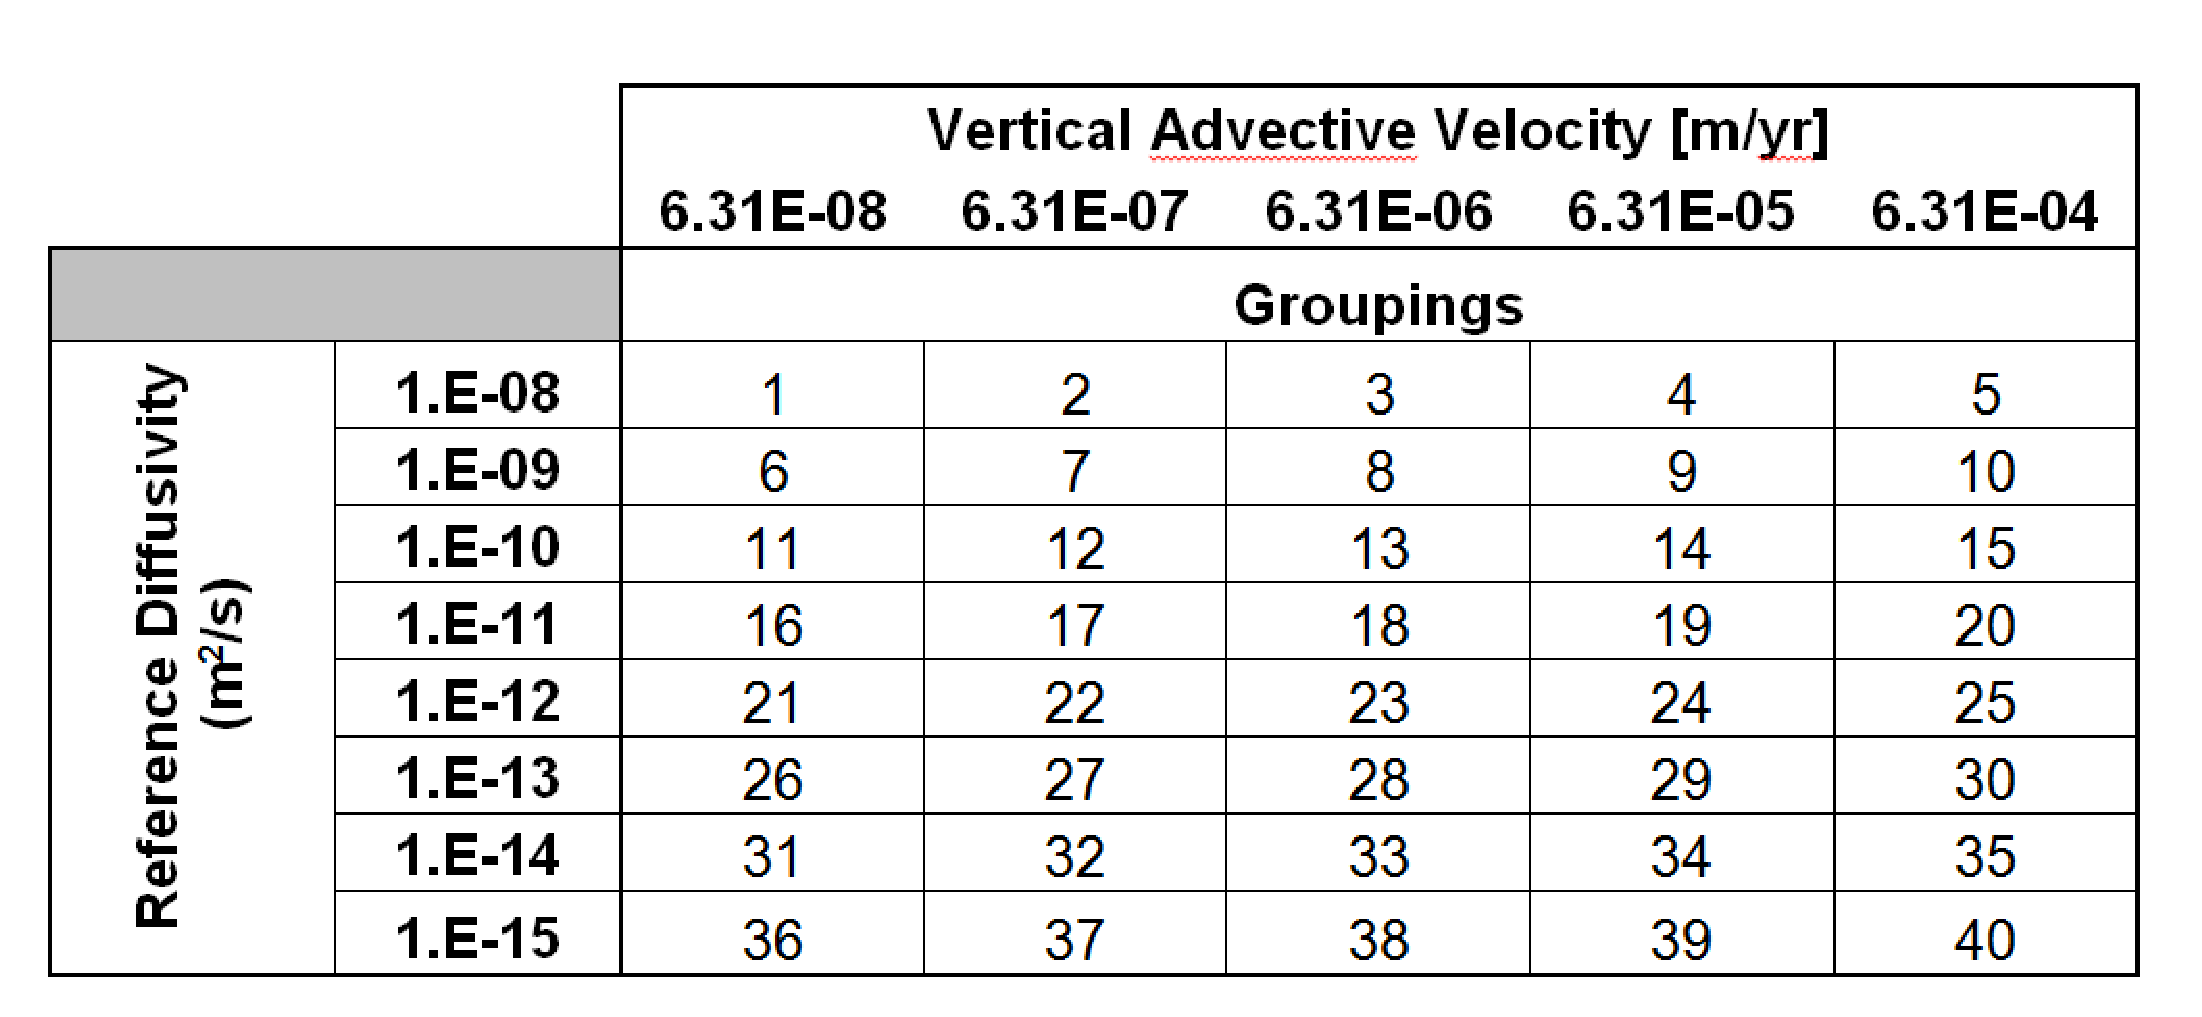
\includegraphics[width=0.7\textwidth]{./chapters/nuclide_sensitivity/clay/AdvVelAndDiffCoeffEBSFail/AdvVelAndDiffCoeffGroups.eps}
\caption{Vertical advective velocity and diffusion coefficient simulation groupings.}
\label{tab:AdvVelAndDiffCoeffGroups}
\end{table}


To capture the importance of the vertical advective velocity, a range was chosen 
to span a number of orders of magnitude between $ 6.31\times 10^{-8}$ 
and $ 6.31\times10^{-4} [m/yr]$. The relative diffusivity was simultaneously varied 
over the eight magnitudes between $ 10^{-8}$ and $ 10^{-15} [m^2/s]$. It is 
worth noting that both the relative diffusivity and the vertical advective 
velocity are functions of porosity in the host rock and are therefore expected 
to vary together. 

%Importantly, the thermal fluxes near the waste have an impact on the dynamic 
%viscosity of the hydraulic medium and can be expected to triple the vertical 
%advective velocity within a clay repository during the heating period 
%\cite{andra_argile:_2005}. %pg 429





\subsection{Thermal Diffusivity Sensitivity Validation}\label{sec:diffusivity}
The thermal diffusivity, $\alpha_{th}$ of geologic repository host media 
describes the tendency of thermal energy to diffuse through, and therefore be 
deposited, in the medium.

\FloatBarrier
\subsubsection{LLNL Model Results}

In the creation of the \gls{STC} database, the thermal diffusivity was varied 
across a broad domain for each isotope, $i$, package spacing, $s$, limiting 
radius $r_{calc}$, and thermal conductivity $K_{th}$, considered.  By 
varying the thermal diffusivity of the disposal system from $0.1-3\times 
10^{-6} [m^2\cdot s^{-1}]$, this sensitivity analysis succeeds in capturing the domain of 
thermal diffusivities witnessed in high thermal diffusivity salt deposits as 
well as low thermal diffusivity clays.

\begin{figure}[htbp!]
\begin{center}
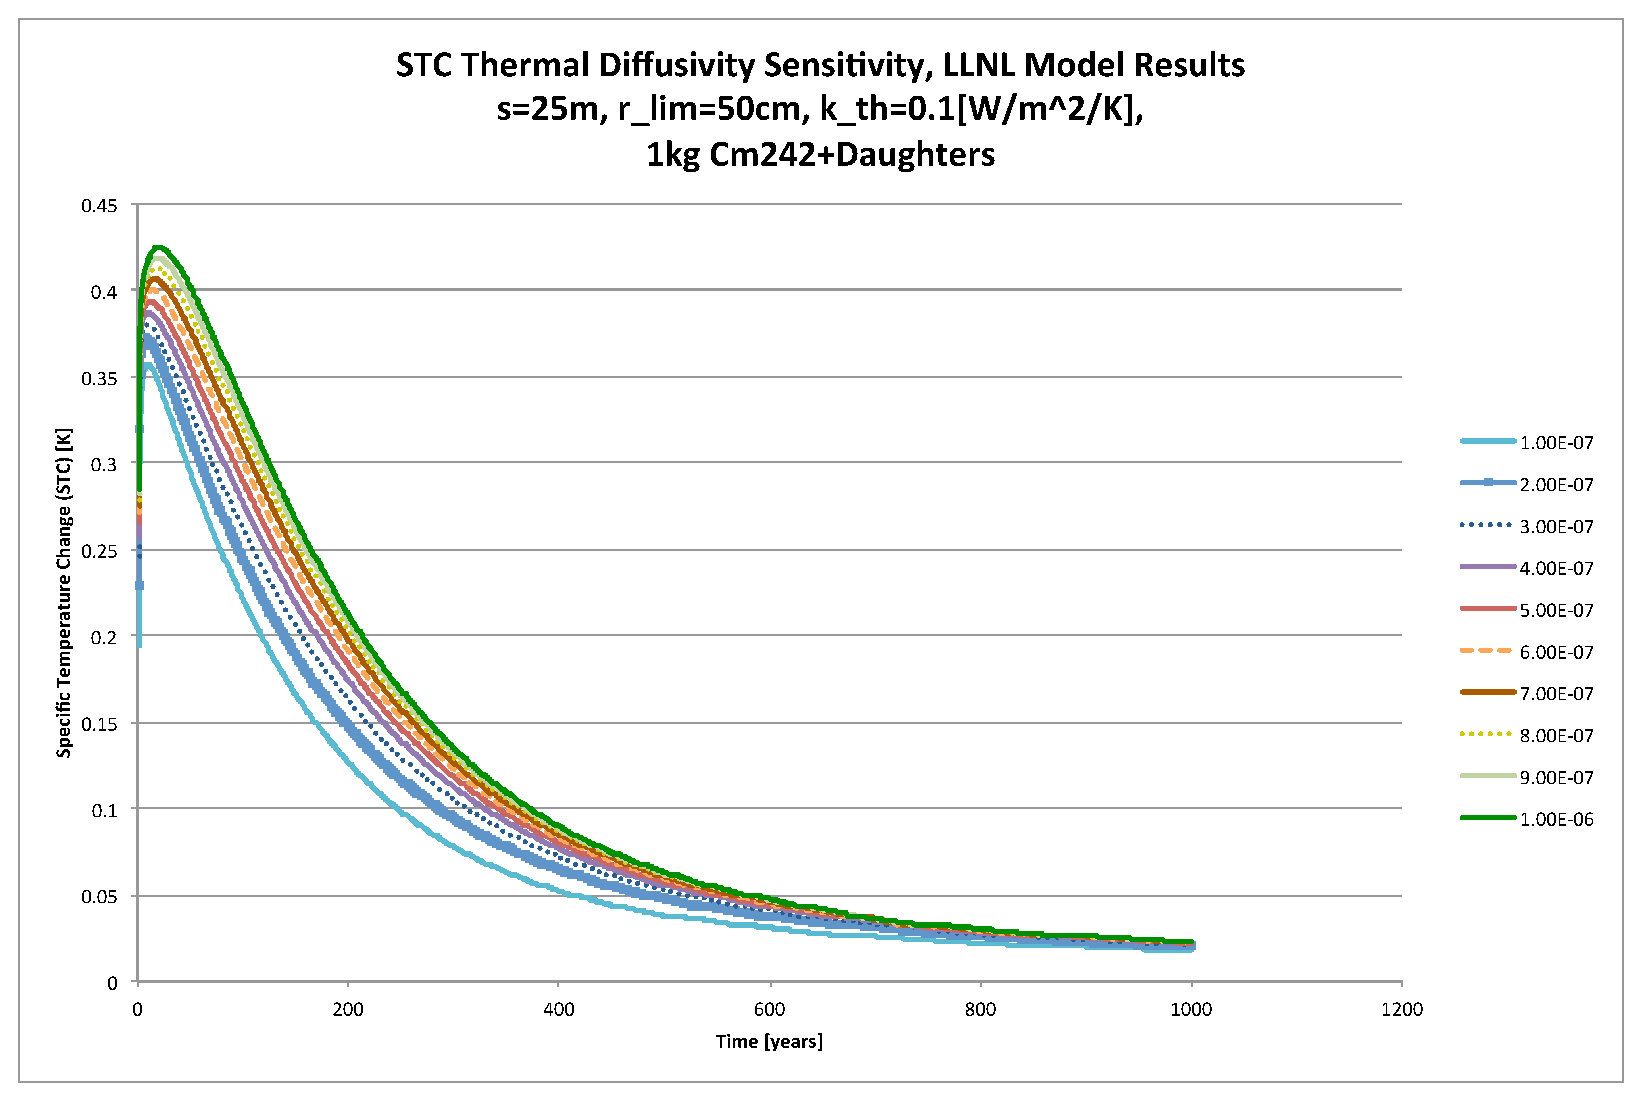
\includegraphics[width=0.7\textwidth]{./chapters/demonstration/diffusivity/Cm242alpha_kth_low.eps}
\end{center}
\caption[$K_{th}$ Sensitivity to $\alpha_{th}$ for low $k_{th}$]{Increased thermal 
diffusivity increases temperatures (here represented by \gls{STC}) in the near field (here $r_{calc} = 0.5m$).}
\label{fig:Cm242alpha_kth_low}
\end{figure}


Figure \ref{fig:Cm242alpha_kth_low} shows the trend in which increased thermal 
diffusivity of a medium increases temperatures in the near field. This 
indicates, then that thermal diffusivity is an important parameter for 
repository geologic medium selection.

%The effect is accentuated by high thermal 
%conductivities, as seen in Figure \ref{fig:Cm242alpha_kth_high}
%
%\begin{figure}[htbp!]
%\begin{center}
%\includegraphics[width=0.7\textwidth]{./chapters/demonstration/diffusivity/Cm242alpha_kth_high.eps}
%\end{center}
%\caption[$K_{th}$ Sensitivity for High $\alpha_{th}$]{Increased thermal diffusivity decreases thermal energy deposition 
%(here represented by \gls{STC}) in the near field (here $r_{calc} = 0.5m$).}
%\label{fig:Cm242alpha_kth_high}
%\end{figure}


\FloatBarrier
\subsubsection{Cyder Results}

In a similar analysis, the thermal diffusivity was compared both with the 
spacing between waste packages and the limiting radius. 

Figures \ref{fig:ar} and \ref{fig:ak} validate the trend noted above that 
increased thermal diffusivity of a medium decreases thermal energy deposition 
in the near field.  Additionally, analysis with the \Cyder STC database 
demonstrates the way in which the importance of $K_{th}$ remains constant, but 
the importance of the limiting radius decreases with increasing $\alpha_{th}$.

\begin{figure}[htbp!]
\begin{center}
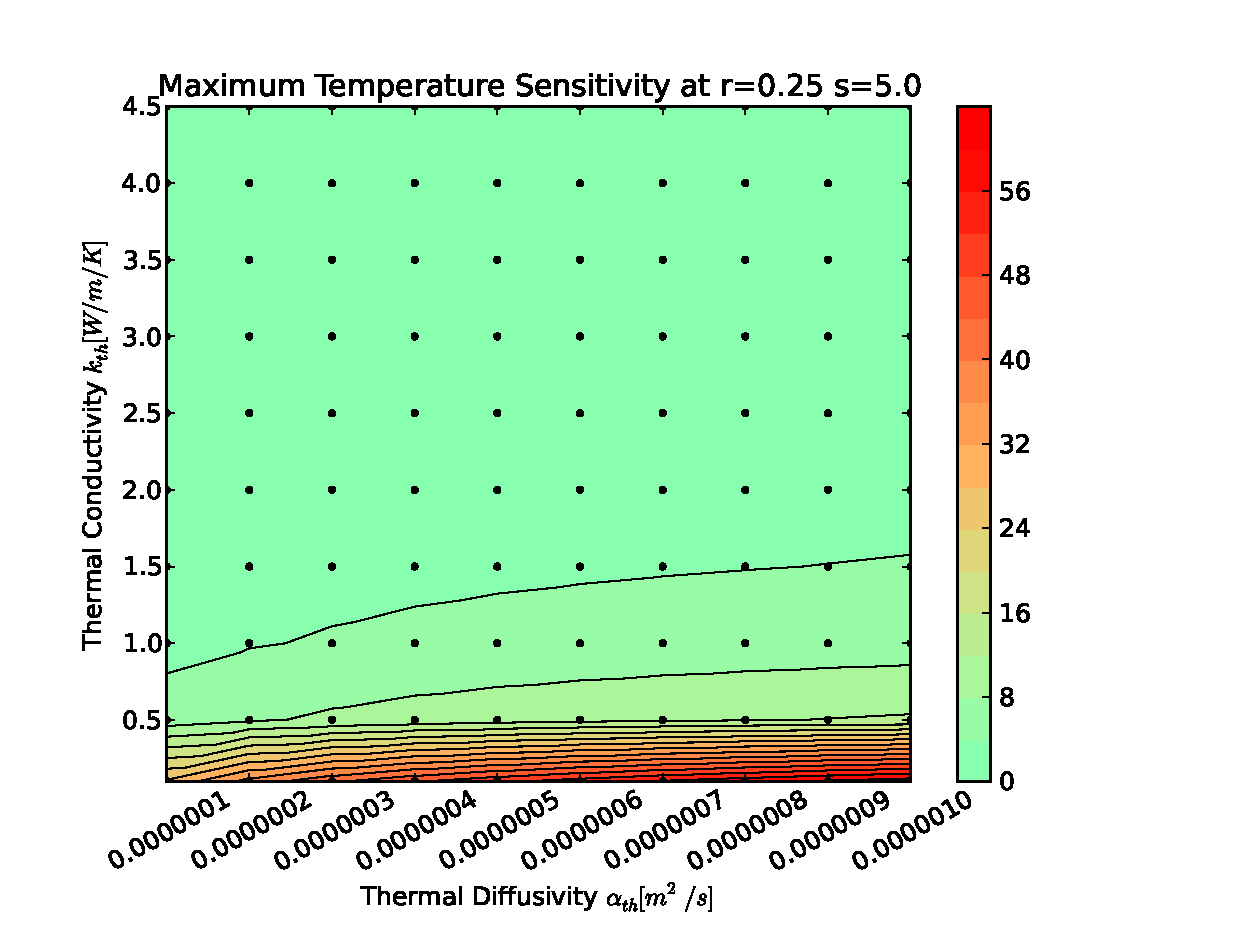
\includegraphics[width=0.7\textwidth]{./chapters/demonstration/diffusivity/ak.eps}
\end{center}
\caption[$\alpha_{th}$ vs. $K_{th}$ Sensitivity in Cyder]{Cyder trends agree
with those of the LLNL model, in which increased thermal diffusivity results in 
decreased thermal deposition in the near field. The above example thermal 
profile results from 10kg of $^{242}Cm$.} 
\label{fig:ar}
\end{figure}


\begin{figure}[htbp!]
\begin{center}
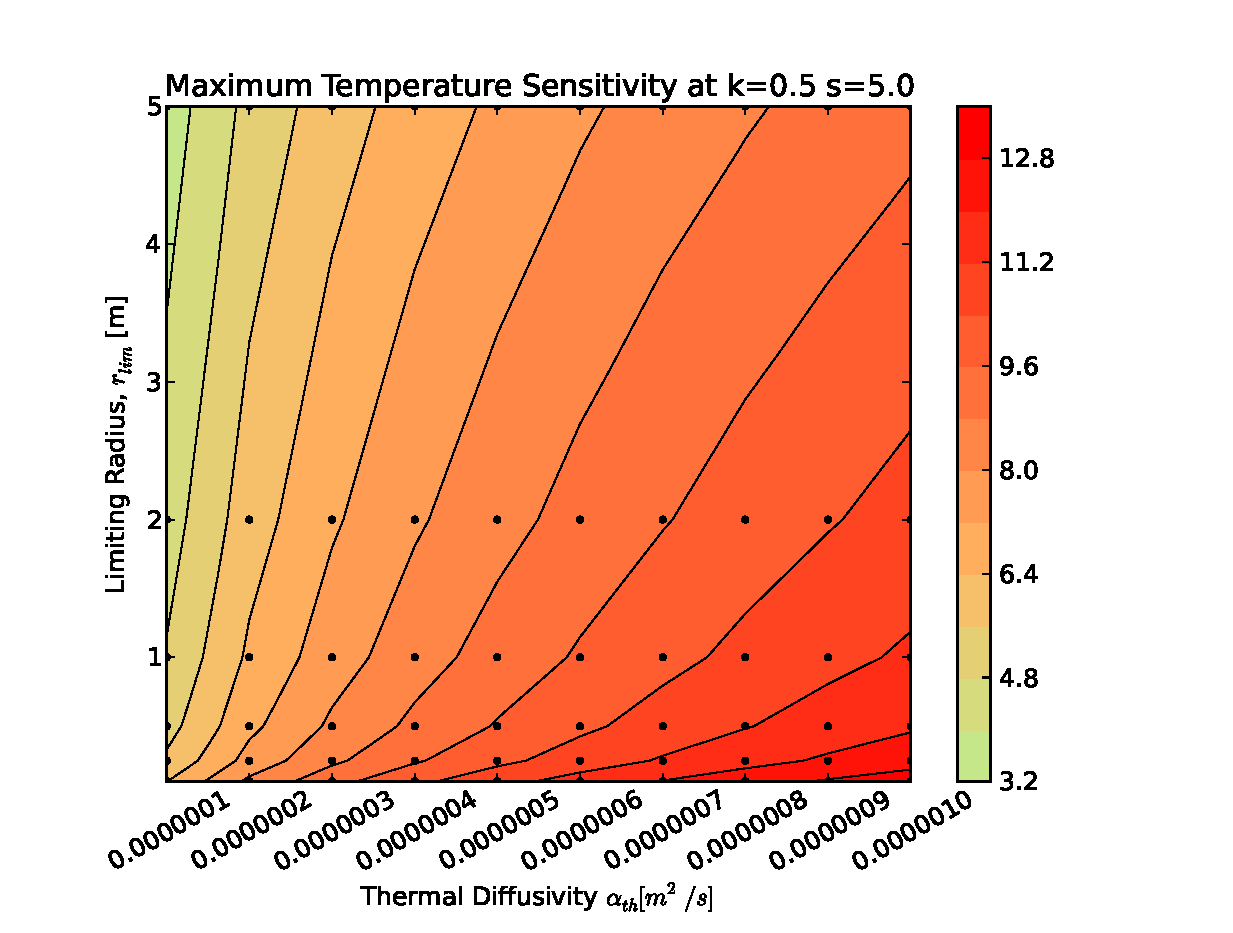
\includegraphics[width=0.7\textwidth]{./chapters/demonstration/diffusivity/ar.eps}
\end{center}
\caption[$\alpha_{th}$ vs. $r_{lim}$ Sensitivity in Cyder]
{Cyder trends agree with 
those of the LLNL model. The importance of the limiting radius decreases with 
increased $K_{th}$. The above example thermal profile results from 10kg of 
$^{242}Cm$}
\label{fig:ak}
\end{figure}


\subsection{Solubility Coefficients}

This study varied the solubility coefficients for each isotope in the simulation 
to help inform the effect of reprocessing on repository benefit for the clay 
repository scenario. The importance of the actinide contribution relative to the 
contribution from $^{129}I$, $^{79}Se$, and $^{99}Tc$ was of particular 
interest.

The dissolution behavior of a solute in an aqueous solutions is called its 
solubility. This behavior is limited by the solute's solubility limit, described  
by an equilibrium constant that depends upon temperature, water chemistry, and 
the properties of the element. The solubility constant for ordinary solutes, 
$K_s$ gives units of concentration, $[kg/m^3]$, and can be determined 
algebraically by the law of mass action which gives the partitioning at 
equilibrium between reactants and products.  For a reaction
\begin{align}
  cC + dD &= yY + zZ,
  \intertext{where}
  c,d,y,z  &= \mbox{ amount of respective constituent }[mol]\nonumber\\
  C,D  &= \mbox{ reactants }[-]\nonumber\\
  Y,Z  &= \mbox{ products }[-]\nonumber,
  \intertext{the law of mass action gives}
  K &= \frac{(Y)^y(Z)^z}{(C)^c(D)^d}
  \intertext{where}
  (X)  &= \mbox{ the equilibrium molal concentration of X }[mol/m^3]\nonumber\\
  K  &= \mbox{ the equilibrium constant }[-].\nonumber
  \label{massaction}
\end{align}
The equilibrium constant for many reactions are known, and can be found in 
chemical tables. Thereafter, the solubility constraints of a solution at 
equilibrium can be found algebraically.  In cases of salts that  dissociate in 
aqueous solutions, this equilibrium constant is called the salt's solubility 
product $K_{sp}$.

This equilibrium model, however, is only appropriate for dilute situations, and 
nondilute solutions at  partial equilibrium must be treated with an activity 
model by substituting the activities of the constituents  for their molal 
concentrations,
\begin{align}
  [X] &= \gamma_x(X)
  \intertext{where}
  [X]  &= \mbox{ activity of X }[-]\nonumber\\
  \gamma_x  &= \mbox{ activity coefficient of X}[-]\nonumber\\
  (X)  &= \mbox{ molal concentration of X}[mol/m^3]\nonumber
  \intertext{such that}
  IAP &= \mbox{ Ion Activity Product }[-].\nonumber\\
      &= \frac{[Y]^y[Z]^z}{[C]^c[D]^d}\\
  \label{IAP}
\end{align}
The ratio between the IAP and the equilibrium constant $(IAP/K)$ quantifiesn
the departure from equilibrium of a solution.  This information is useful during 
the transient stage in which a solute is first introduced to a solution. When 
$IAP/K<1$, the solution is undersaturated with respect to the products. When, 
conversely, $IAP/K>1$, the solution is oversaturated and precipitation of solids 
in the volume will occur. 

\subsubsection{Parametric Range}

The solubility coefficients were varied in this simulation using a multiplier. 
The reference solubilities for each element were multiplied by the multiplier 
for each simulation group. This technique preserved relative solubility among 
  elements. Forty values of solubility coefficient multiplier were used to change 
the far field solubility. This did not alter any of the solubility in the
EDZ, WF, or Fast Path solubilities.

The values of the solubility multiplier were deliberately varied over many 
magnitudes, from $1\time10^{-9}$ through $5\times10^{10}$. This multiplier
multiplied the most likely values of solubility for each element, so 
the relative solubility between elements was preserved.


\subsubsection{Results}

The results for varying the solubility coefficient were very straightforward.  
For solubility limits below a certain threshold, the dose releases were directly 
proportional to the solubility limit, indicating that the radionuclide 
concentration saturated the groundwater up to the solubility limit near the 
waste form.  For solubility limits above the threshold, however, further 
increase to the limit had no effect on the peak dose. This demonstrates the 
situation in which the solubility limit is so high that even complete 
dissolution of the waste inventory into the pore water is insufficient to reach 
the solubility limit.

In Figures \ref{fig:SolSumFactor} and \ref{fig:SolSum}, it is clear that for 
solubility constants lower than a threshold, the relationship between peak 
annual dose and solubility limit is strong.

\begin{figure}[ht]
\centering
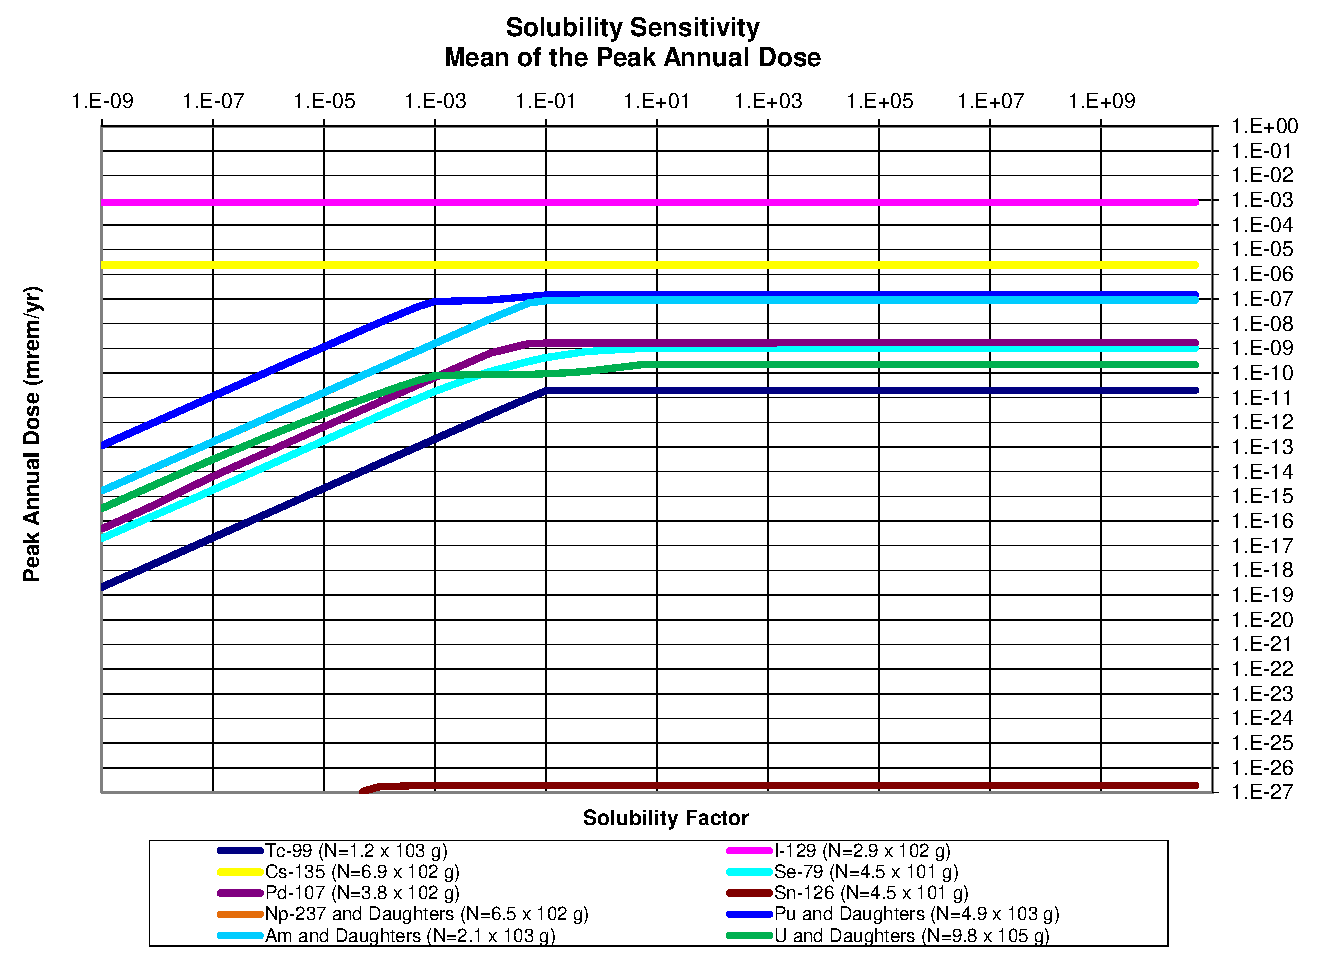
\includegraphics[width=\linewidth]{./chapters/nuclide_sensitivity/clay/Solubility/Solubility_Summary_SolFactor.eps}
\caption{Solubility factor sensitivity. The peak annual dose due to an inventory, 
$N$, of each isotope.}
\label{fig:SolSumFactor}
\end{figure}

\begin{figure}[ht]
\centering
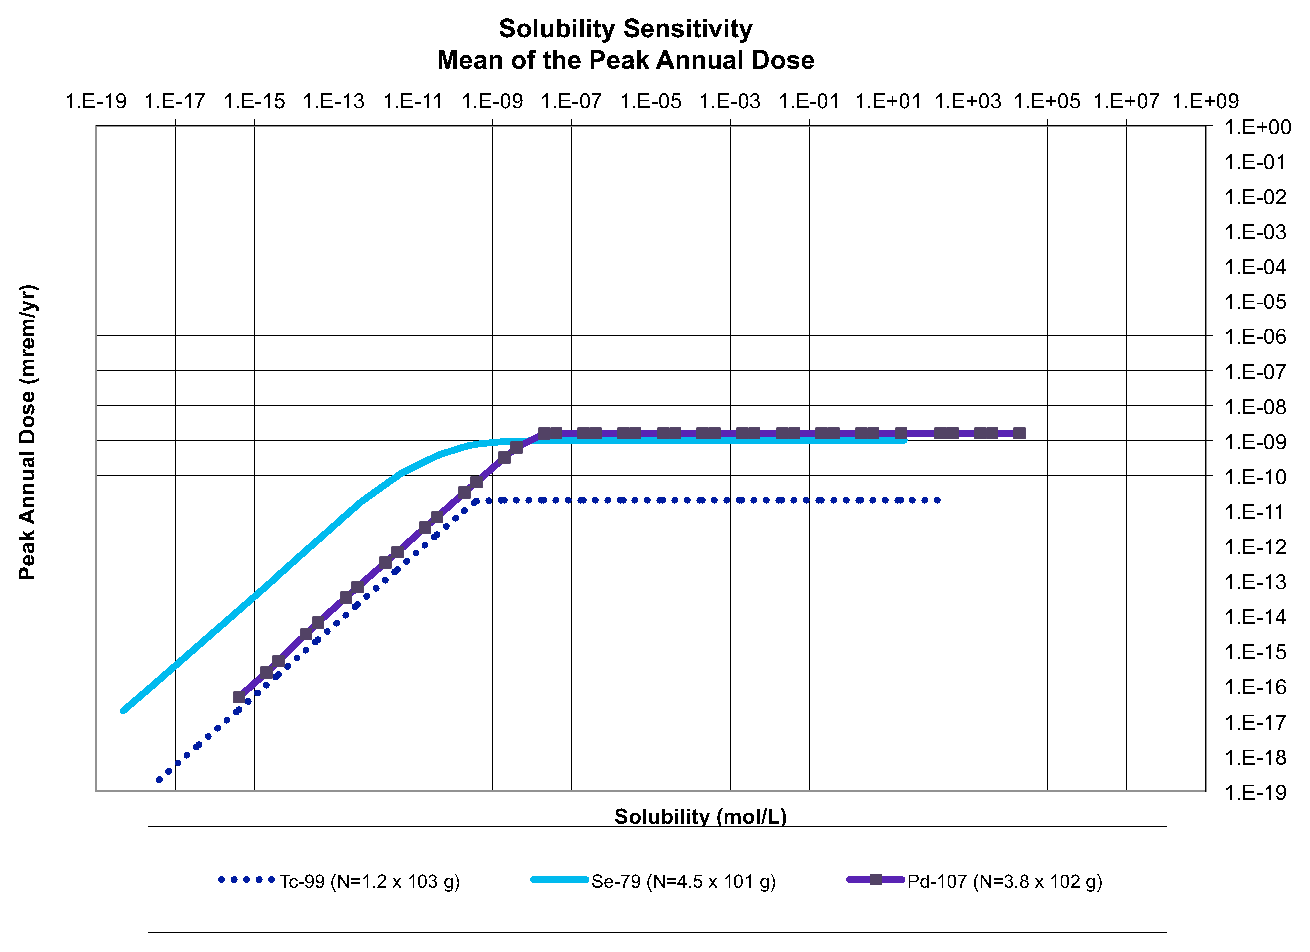
\includegraphics[width=\linewidth]{./chapters/nuclide_sensitivity/clay/Solubility/Solubility_Summary_Sol.eps}
\caption{Solubility limit sensitivity. The peak annual dose due to an inventory, 
$N$, of each isotope.}
\label{fig:SolSum}
\end{figure}
\clearpage



\subsection{The Partition Coefficient}

This analysis investigated the peak dose rate contribution from various 
radionuclides to the partition coefficient of those radionuclides. 

The partition or distribution coefficient, $K_d$, relates the amount of contaminant adsorbed into the 
solid phase of the host medium to the amount of contaminant adsorbed into the 
aqueous phase of the host medium. It is a common empirical coefficient used to 
capture the effects of a number of retardation mechanisms. The coefficient 
$K_d$, in units of $[m^3\cdot kg^{-1}]$, is the ratio of the mass of contaminant in the 
solid to the mass of contaminant in the solution.

The retardation factor, $R_f$, which is the ratio between velocity of water through a 
volume and the velocity of a contaminant through that volume, can be expressed 
in terms of the partition coefficient,

\begin{align}
  R_f &= 1+\frac{\rho_b}{n_e}K_d
  \label{retardation}
  \intertext{where}
  \rho_b &= ~~\mbox{bulk density}[kg\cdot m^{-3}]\nonumber
  \intertext{and}
  n_e &= ~~\mbox{effective porosity of the medium}[\%].\nonumber
\end{align}




\subsubsection{Parametric Range}

The parameters in this model were all set to the default values except a multiplier 
applied to the partitioning $K_d$ coefficients.

The multiplier took the forty values $1\times10^{-9}, 5\times10^{-8}, \cdots 
5\times10^{10}$ Only the far field partition coefficients were altered by this 
factor. Partition coefficients effecting the EDZ and fast pathway were not 
changed.


\subsubsection{Results}

The expected inverse relationship between the retardation 
factor and resulting peak annual dose was found for all elements that were not 
assumed to be effectively infinitely soluble. In the low retardation coefficient 
cases, a regime is established in which the peak annual dose is entirely 
unaffected by changes in retardation coefficient. For large values of 
retardation coefficient, the sensitivity to small changes in the retardation 
coefficient increases dramatically. In that sensitive regime, the change in peak 
annual dose is inversely related to the retardation coefficient. Between these 
two regimes was a transition regime, in which the $K_d$ factor ranges from $1\times10^{-5}$ to 
$5\times10^{0} [-]$.

It is clear from Figures \ref{fig:KdSumFactor} and \ref{fig:KdSum} that 
for retardation coefficients greater than a threshold, the 
relationship between peak annual dose and retardation coefficient is a strong 
inverse one. 

\begin{figure}[ht]
\centering
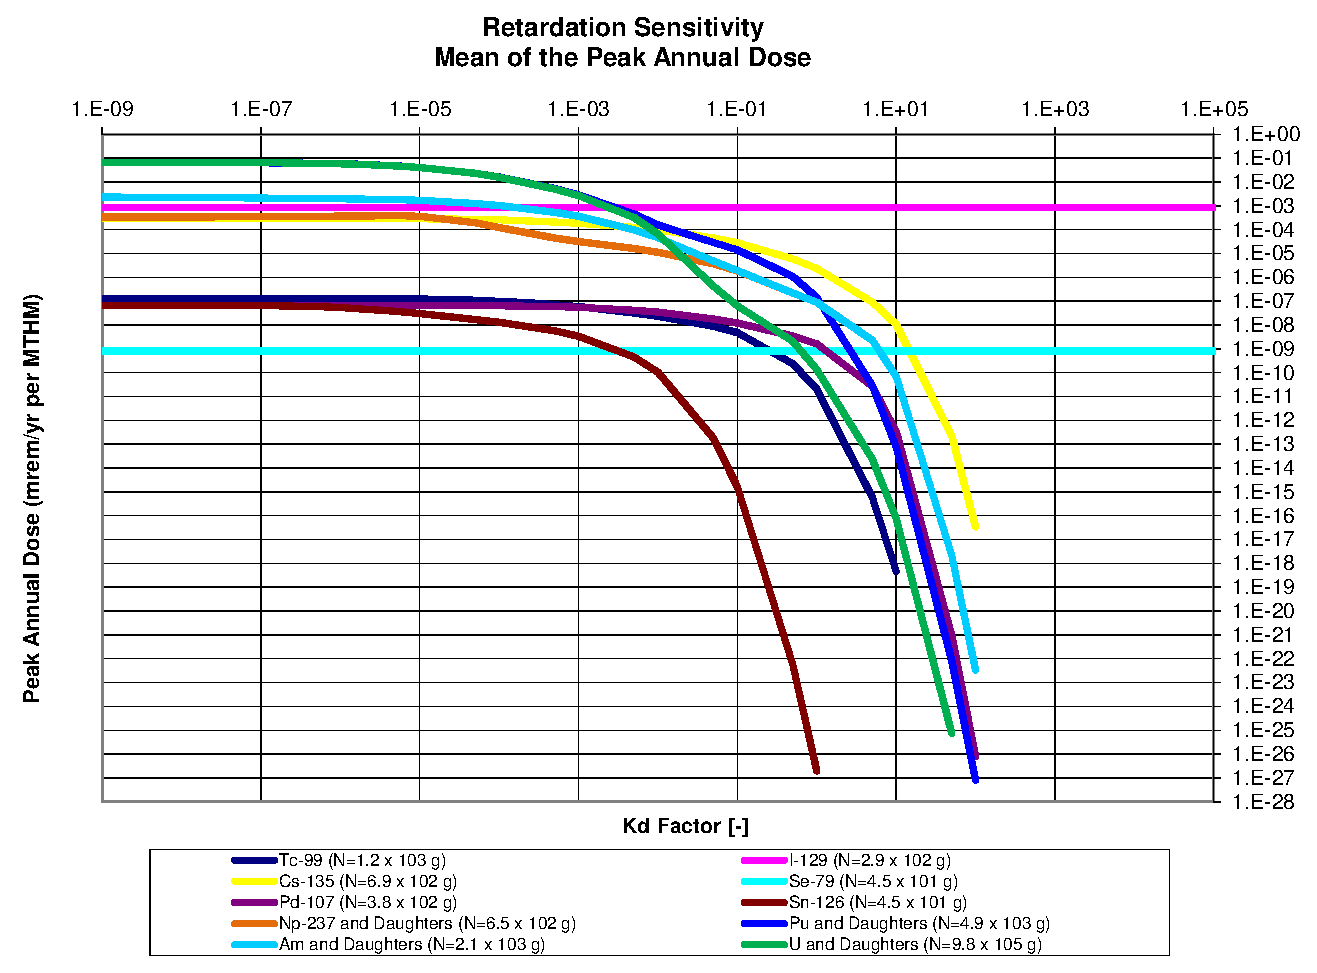
\includegraphics[width=\linewidth]{./chapters/nuclide_sensitivity/clay/Sorption/Retardation_Summary_kdFactor.eps}
\caption{$K_d$ factor sensitivity.  The peak annual dose due to an inventory, 
$N$, of each isotope.}
\label{fig:KdSumFactor}
\end{figure}

\begin{figure}[ht]
\centering
\includegraphics[width=\linewidth]{./chapters/nuclide_sensitivity/clay/Sorption/Retardation_Summary_kd.eps}
\caption{$K_d$ sensitivity.  The peak annual dose due to an inventory, 
$N$, of each isotope.}
\label{fig:KdSum}
\end{figure}

\clearpage


\subsection{Waste Form Degradation Rate}
\label{sed:wfdeginv}


The sensitivity of peak dose rate to the waste form degradation rate was 
determined with respect to varying inventories of waste.

The sensitivity of repository performance to waste form degradation rate was
expected to vary according to the waste inventory. For cases in which the dominant dose contributing 
radionuclides have half-lives much shorter than the expected waste form lifetime, 
the waste form degradation rate is not expected to have an effect. So too, for 
cases in which the primary barrier to release, the slow diffusive pathway, 
dominates overall repository performance, the waste form engineered barrier was
expected to have a negligible effect on repository performance in comparison.

In the case of a clay repository, the effect of the long time scale of the 
diffusive release pathway was to dampen the potential effect of high waste form 
degradation rates. 

\subsubsection{Parametric Range}

These runs varied the waste form degradation rate and the waste inventory mass 
factor.  There were forty runs corresponding to eight values of the waste form degradation 
rate and five values of the mass factor.

The waste form degradation rate was varied over the eight magnitudes 
between $10^{-9}$ and $10^{-2} [1/yr]$. The inventory mass factor was varied 
over the five magnitudes between $0.001$ and $10.0 [-]$. 

\subsubsection{Safety Indicators}
Safety indicators for post closure repository performance have been developed by 
the \gls{UFD} campaign which utilize the inventory multiplier that was varied in 
this study \cite{nutt_generic_2009}. These indicators are normalized by a 
normalization factor (100 mrem/yr) recommended by the \gls{IAEA} as the limit to 
``relevant critical members of the public'' \cite{international_atomic_energy_agency_international_1996}. The functional form for 
this safety indicator for a single waste category, \gls{HLW}, is just 

\begin{align}
SI_{G} &= \left(\frac{\sum_{i=1}^{N}D_{G,i}(I_i, F_{d})}{100mrem/yr}\right)[GWe/yr].
\label{indicator}
\intertext{where}
SI_{G} &= \mbox{Safety indicator for disposal in media type G}[GWe/yr]\nonumber\\
N &= \mbox{Number of key radionuclides considered in this indicator}\nonumber\\
D_{G,i} &= \mbox{Peak dose rate from isotope i in media type G}[mrem/yr]\nonumber\\
F_{d} &= \mbox{Fractional waste form degradation rate}[1/yr].\nonumber
\end{align}

Tables \ref{tab:WFDegIndicatorsTcICsSeCl}, 
\ref{tab:WFDegIndicatorsPdSnZrNb}, and 
\ref{tab:WFDegIndicatorsActinides} report the safety indicators for 
various independent isotopes and, where applicable, their daughters. 

\begin{table}[h!]
\centering
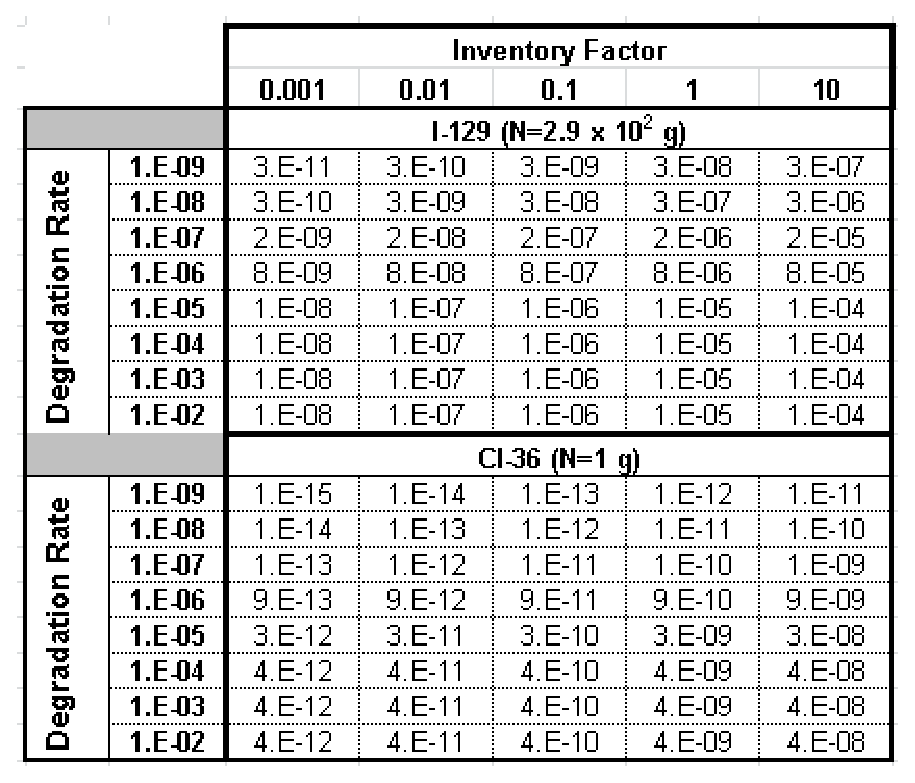
\includegraphics[width=0.5\textwidth]{./chapters/nuclide_sensitivity/clay/WFDegAndInv/IndicatorsSolNonSorbing.eps}
\caption{Safety indicators for soluble, non-sorbing nuclides.} 
\label{tab:WFDegIndicatorsTcICsSeCl}
\end{table}

\begin{table}[h!]
\centering
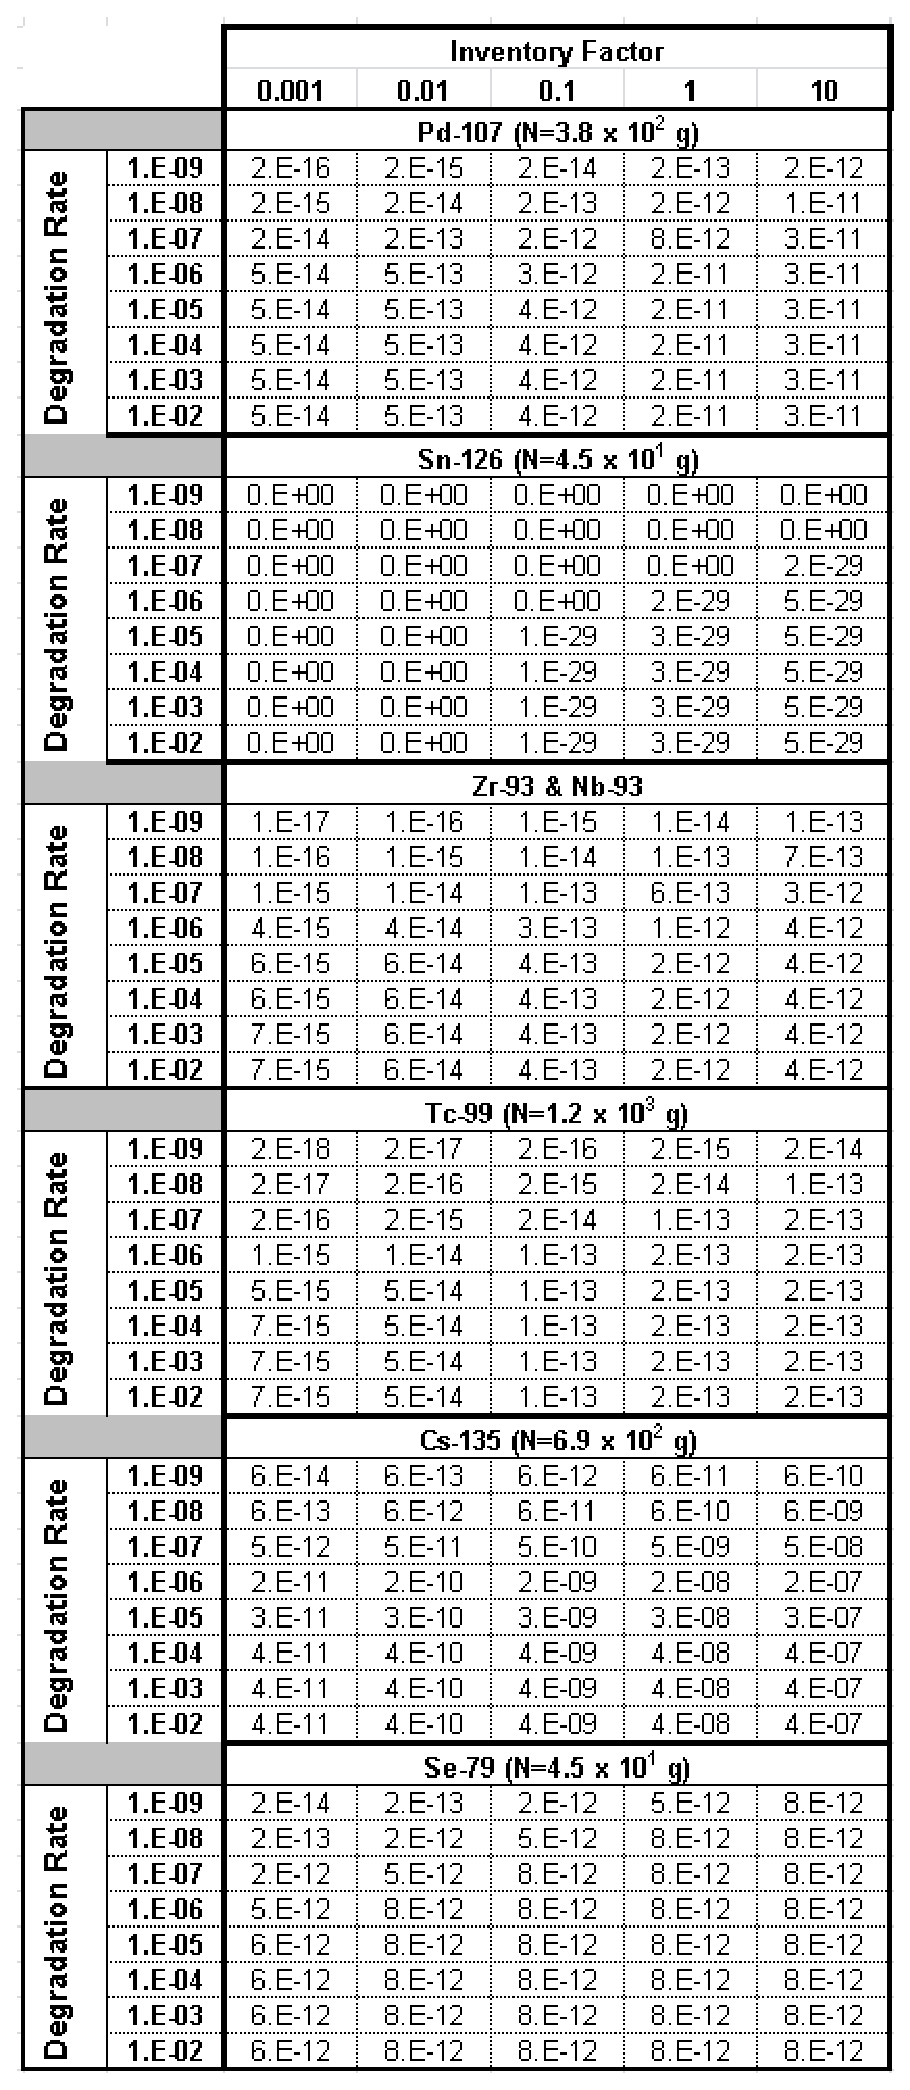
\includegraphics[width=0.5\textwidth]{./chapters/nuclide_sensitivity/clay/WFDegAndInv/IndicatorsSolLimSorbing.eps}
\caption{Safety indicators for solubility limited and sorbing nuclides.} 
\label{tab:WFDegIndicatorsPdSnZrNb}
\end{table}

\begin{table}[h!]
\centering
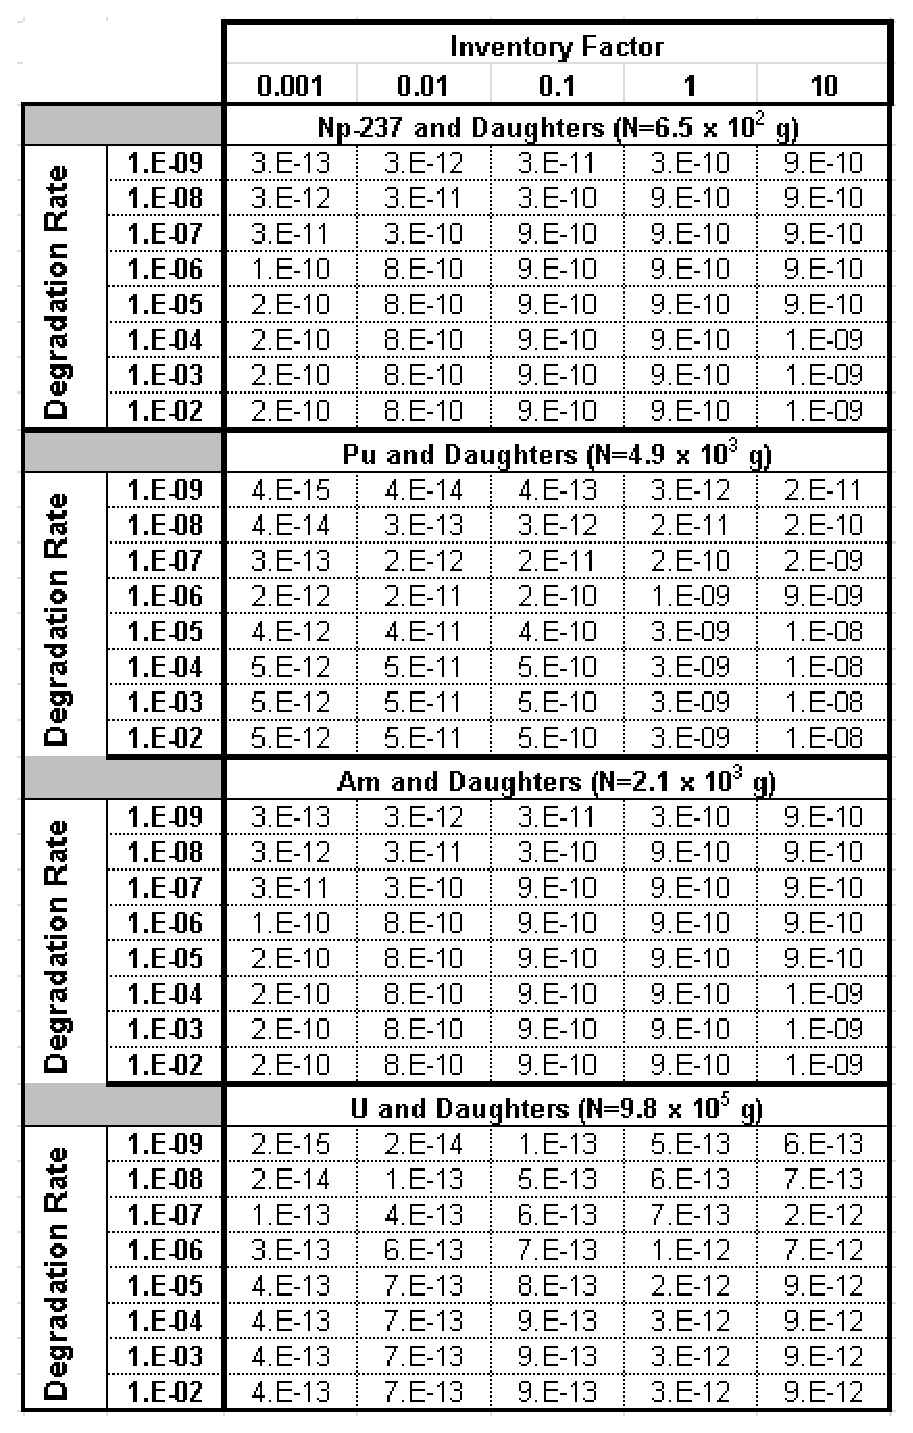
\includegraphics[width=0.5\textwidth]{./chapters/nuclide_sensitivity/clay/WFDegAndInv/IndicatorsActinides.eps}
\caption{Safety indicators for the actinides and their daughters.}
\label{tab:WFDegIndicatorsActinides}
\end{table}

\clearpage 


\subsection{Waste Package Failure Time}
\label{sec:wpfail}

The time of waste package failure was not expected to greatly affect the 
magnitude of the mean of the peak doses except for cases in which waste package failure times 
exceeded the half lives of dominant dose-contributing nuclides. 
That is, since the dominant dose-contributing 
radionuclides for the reference case are quite long lived ($^{129}I$, etc.), 
all but the longest reasonable waste package containment lifetime is overwhelmed by 
the half life of the dominant radionuclides. The long time scales of 
radionuclide release was expected to render the the waste package lifetime 
irrelevant if it was shorter than a million years. 

Though the model contains a unit cell-type model, it is possible to determine, 
in post processing, the results of a simulation with temporally heterogeneous 
failures among waste packages. That is, by a weighted sum of the time histories 
of the no-fail case and the all-fail case, it is possible to mimic a 
time-varying failure among the many waste packages. 

\subsubsection{Parametric Range}

To investigate the effect of the waste package failure time, it was varied over 
five magnitudes from one thousand to ten million years. Simultaneously, the reference 
diffusivity was varied over the eight magnitudes between $1\times10^{-8}$ and 
$1\times10^{-15}$ in order to determine the correlation between increased 
radionuclide mobility and the waste package lifetime. 




\chapter{Thermal Transport Sensitivity Analysis}\label{ch:thermal_sensitivity}

The results here provide an overview of the relative importance of thermal
parameters that affect the repository capacity of simplified generic
disposal concept in various geologic media where conduction is the dominant
heat transfer mode. The applicability of this sensitivity analysis is thus
restricted to enclosed, backfilled concepts.  

\subsection{Parametric Domain}

Sensitivity analyses were conducted which span the parametric range of values 
generated by the reference specific temperature change database and described 
in Table \ref{tab:thermal_cases}.  

\begin{table}[ht!]
\centering
\footnotesize{
\begin{tabular}{|l|l|l|r|}
\multicolumn{4}{c}{\textbf{Thermal Cases}}\\
\hline
\textbf{Parameter} & \textbf{Symbol} & \textbf{Units} & \textbf{Value Range} \\
\hline
Diffusivity & $\alpha_{th}$ & $[m^2\cdot s^{-1}]$ & $1.0\times10^{-7}-3.0\times10^{-6}$\\
\hline
Conductivity & $K_{th}$     & $[W\cdot m^{-1} \cdot K^{-1}]$ & $0.1 - 4.5$ \\
\hline
Spacing & $S$ & $[m]$ & 2, 5, 10, 15, 20, 25, 50 \\
\hline
Radius & $r_{lim}$ & $[m]$ & 0.1, 0.25, 0.5, 1, 2, 5 \\
\hline
Isotope & $i$ & $[-]$ & $^{241,243}Am,$  \\
        & & & $^{242,243,244,245,246}Cm,$  \\
        & & & $^{238,240,241,242}Pu$  \\
        & & & $^{134,135,137}Cs$  \\
        & & & $^{90}Sr$  \\
\hline
\end{tabular}
\caption{A thermal reference dataset of \gls{STC} values as a function of each of these parameters was generated by repeated parameterized runs of the LLNL 
MathCAD model\cite{greenberg_application_2012, greenberg_investigations_2012}.}
\label{tab:thermal_cases}
}
\end{table}



These values were selected to provide detail in the near field and at values of
$\alpha_{th}$ and $K_{th}$ in the three host media under consideration in this
work.

\subsection{Approach}

% used existing gdsms 
This analysis utilized the \gls{LLNL} semi-analytic MathCAD model
discussed in Section \ref{sec:llnl_background}.  It performs detailed
calculations of the conductive thermal transport in a generic repository
concept with a gridded layout.  

It relies on the thermal diffusivity, $\alpha_{th}$ and conductivity $K_{th}$ of 
the material as well as the waste package spacing, $S$, and thermally limiting 
radius, $r_{lim}$. Finally, it relies on the \gls{STC} data calculated with the 
semi-analytic model based on the decay heat profiles of the emplaced wastes, $Q$. 
The essential decay heat profiles, $Q$, were retrieved from a \gls{UFD} database 
provided by Carter et al. \cite{carter_fuel_2011}.



\section{Isotopic Thermal Sensitivity Study}\label{sec:isotopic}

\section{Thermal Conductivity Sensitivity Validation}\label{sec:conductivity}
The thermal conductivity, $K_{th}$ of geologic repository host media impacts 
the speed of transport, and therefore the time evolution of thermal energy 
deposition, in the medium. 

\FloatBarrier
\subsection{LLNL Model Results}
In the creation of the \gls{STC} database, the thermal conductivity was varied 
across a broad domain for each isotope, $i$, package spacing, $s$, limiting 
radius $r_{calc}$, and thermal diffusivity $\alpha_{th}$, considered.  By 
varying the thermal conductivity of the repository model from 0.1 to 4.5
$[W\cdot m^{-1} \cdot K^{-1}]$, this sensitivity analysis succeeds in capturing the domain of 
thermal conductivities witnessed in high thermal conductivity salt deposits as 
well as low thermal conductivity clays.

\begin{figure}[htbp!]
\begin{center}
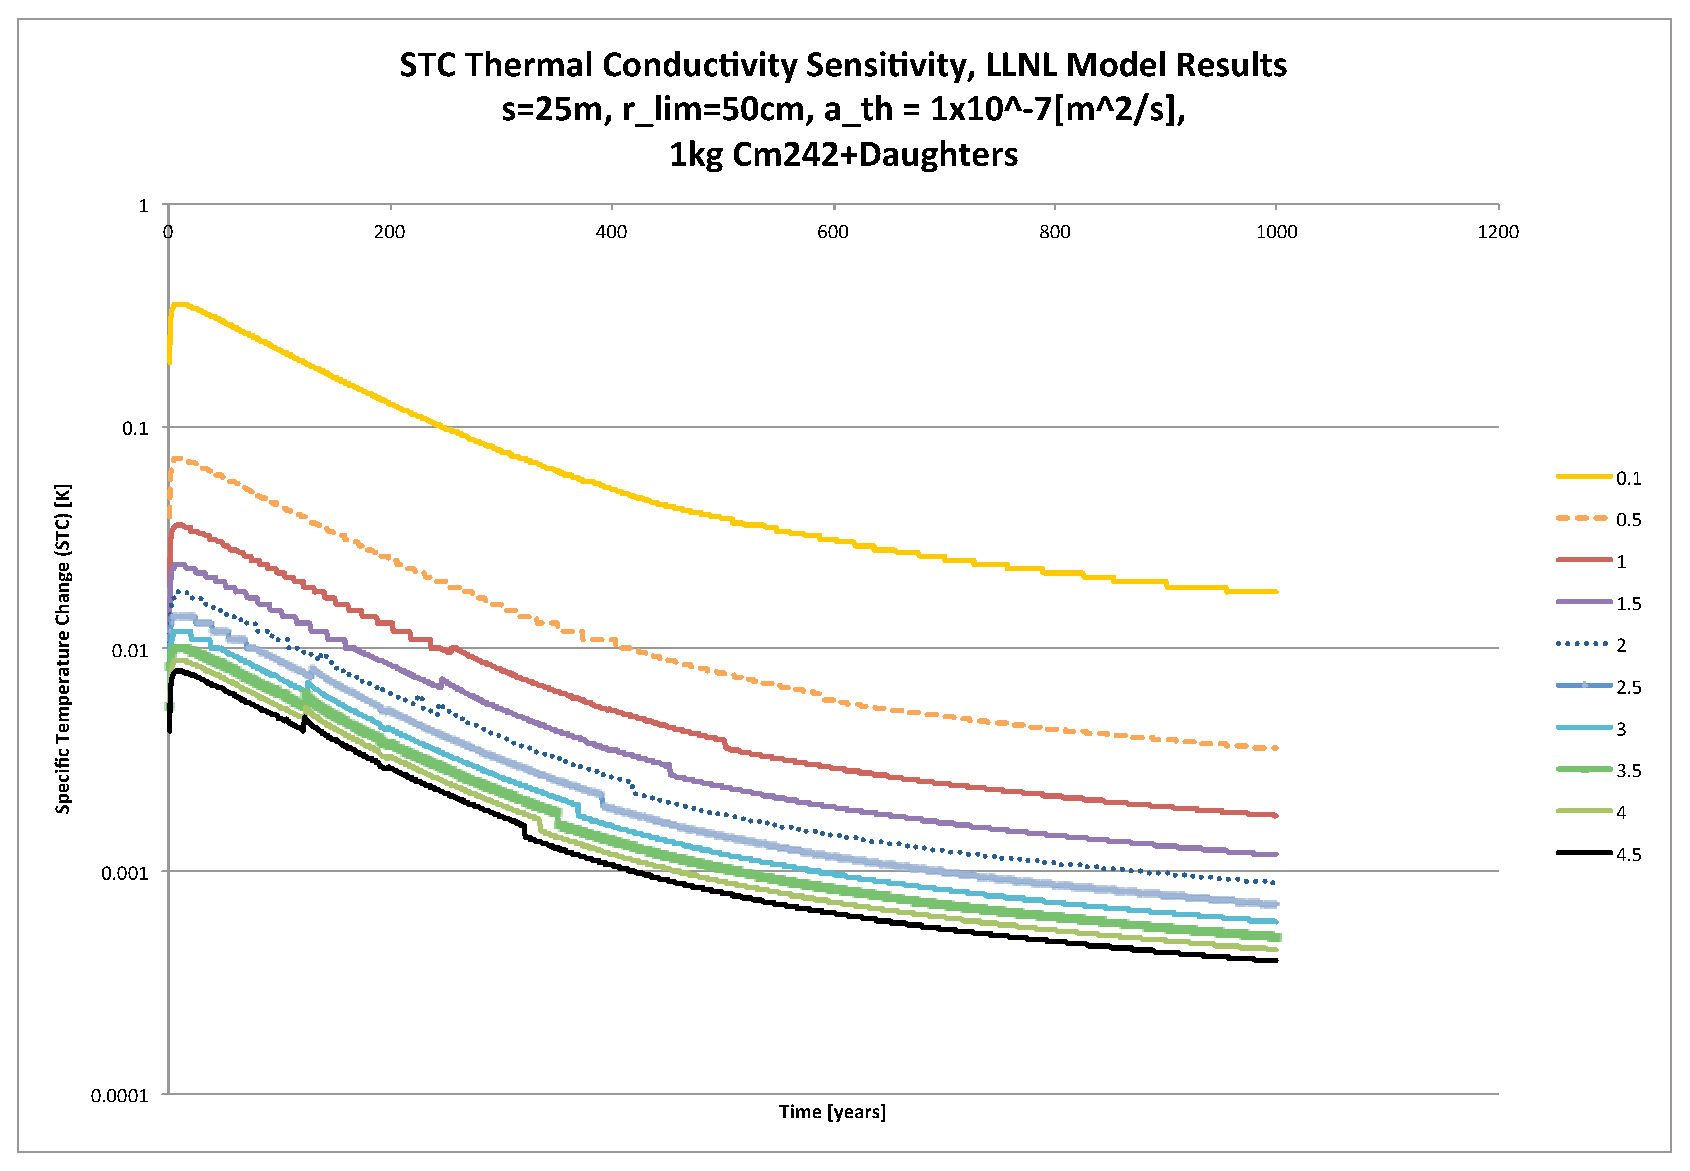
\includegraphics[width=0.7\textwidth]{./chapters/demonstration/conductivity/Cm242kth_alpha_low.eps}
\end{center}
\caption[$K_{th}$ Sensitivity for Low $\alpha_{th}$ in LLNL Model]{Increased thermal conductivity decreases thermal energy deposition 
(here represented by \gls{STC}) in the near field (here $r_{calc} = 0.5m$).}
\label{fig:Cm242Kth_alpha_low}
\end{figure}

Figure \ref{fig:Cm242Kth_alpha_low} shows the trend in which increased thermal conductivity of a medium decreases thermal energy 
deposition in the near field. This indicates, then that thermal conductivity is 
an important parameter for repository geolgic medium selection. 

\FloatBarrier
\subsection{Cyder Results}

In a similar analysis, the thermal conductivity was compared both with the 
spacing between waste packages and the limiting radius. 

Figures \ref{fig:kr} and \ref{fig:ks} validate the trend noted above that 
increased thermal conductivity of a medium decreases thermal energy deposition 
in the near field.  Additionally, analysis with the \Cyder STC database 
demonstrates the way in which the importance of spacing and the importance of 
the limiting radius decrease with increasing $K_{th}$.

\begin{figure}[htbp!]
\begin{center}
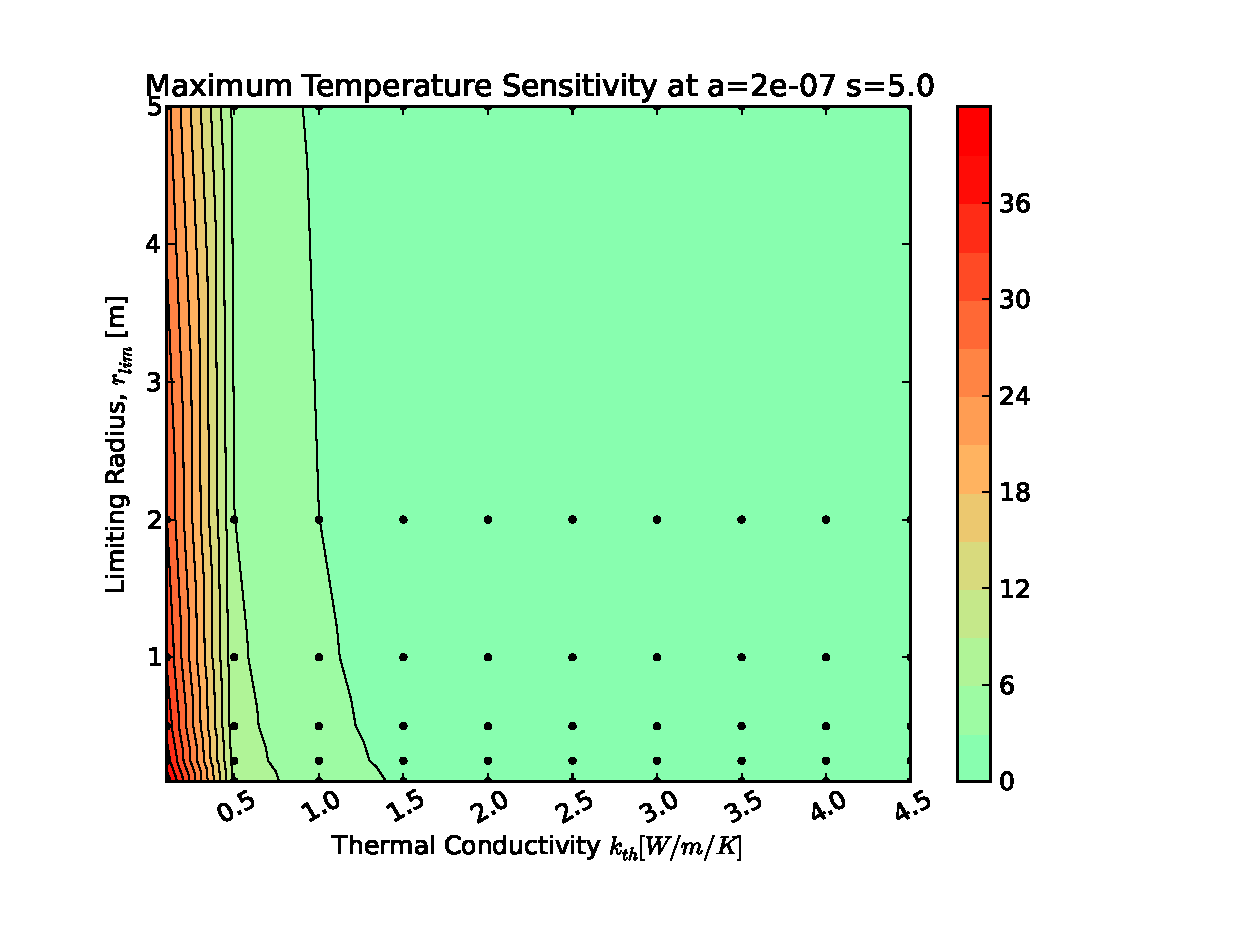
\includegraphics[width=0.7\textwidth]{./chapters/demonstration/conductivity/kr.eps}
\end{center}
\caption[$K_{th}$ vs. $r_{lim}$ Sensitivity in Cyder]
{Cyder results agree with 
those of the LLNL model. The importance of the limiting radius decreases with 
increased $K_{th}$. The above example thermal profile results from 10kg of 
$^{242}Cm$}
\label{fig:kr}
\end{figure}

\begin{figure}[htbp!]
\begin{center}
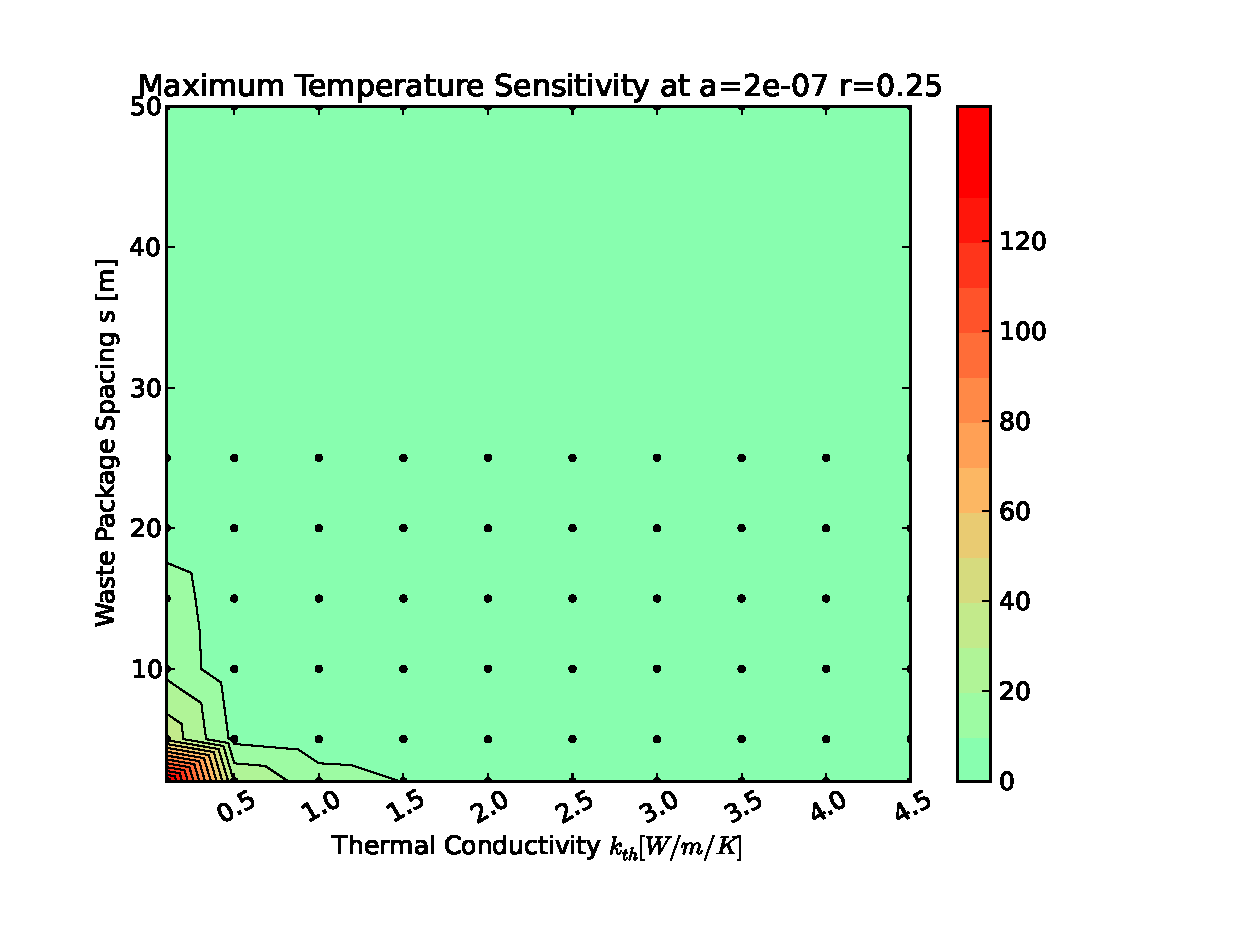
\includegraphics[width=0.7\textwidth]{./chapters/demonstration/conductivity/ks.eps}
\end{center}
\caption[$K_{th}$ vs. Waste Package Spacing Sensitivity in Cyder]{Cyder results agree with 
those of the LLNL model. The importance of the limiting radius decreases with 
increased $K_{th}$. The above example thermal profile results from 10kg of 
$^{242}Cm$}
\label{fig:ks}
\end{figure}



\subsection{Thermal Diffusivity Sensitivity Validation}\label{sec:diffusivity}
The thermal diffusivity, $\alpha_{th}$ of geologic repository host media 
describes the tendency of thermal energy to diffuse through, and therefore be 
deposited, in the medium.

\FloatBarrier
\subsubsection{LLNL Model Results}

In the creation of the \gls{STC} database, the thermal diffusivity was varied 
across a broad domain for each isotope, $i$, package spacing, $s$, limiting 
radius $r_{calc}$, and thermal conductivity $K_{th}$, considered.  By 
varying the thermal diffusivity of the disposal system from $0.1-3\times 
10^{-6} [m^2\cdot s^{-1}]$, this sensitivity analysis succeeds in capturing the domain of 
thermal diffusivities witnessed in high thermal diffusivity salt deposits as 
well as low thermal diffusivity clays.

\begin{figure}[htbp!]
\begin{center}
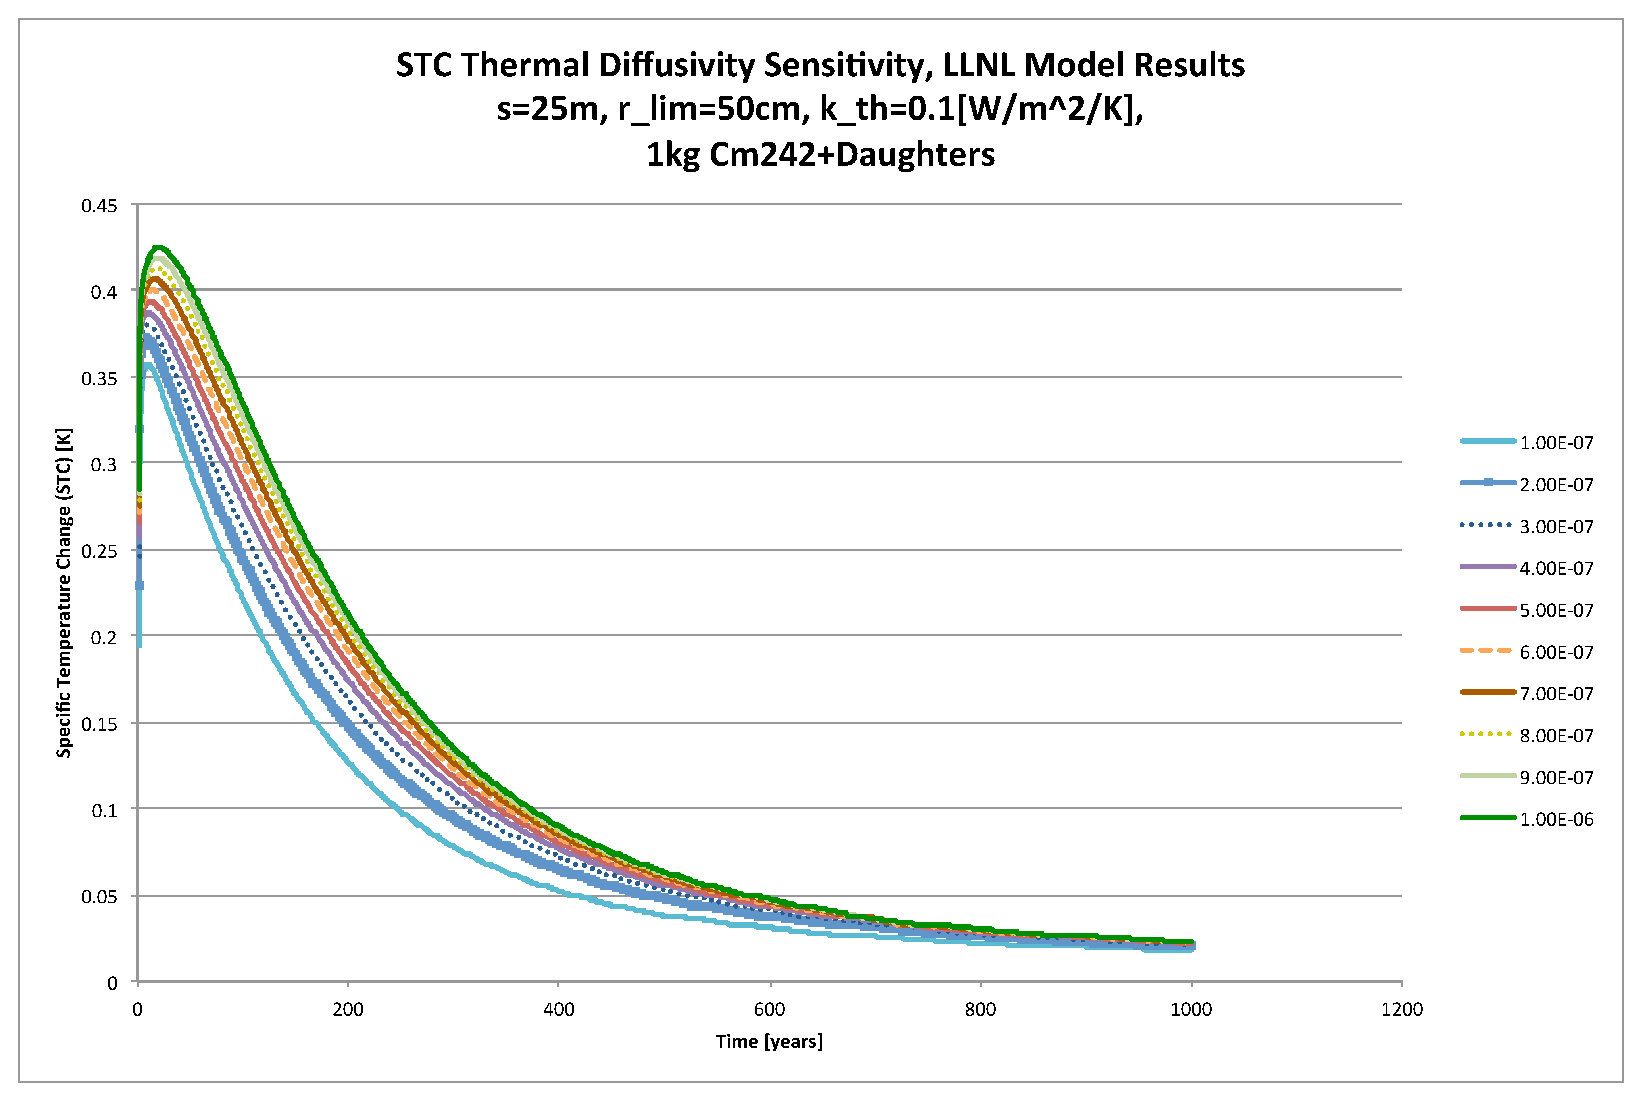
\includegraphics[width=0.7\textwidth]{./chapters/demonstration/diffusivity/Cm242alpha_kth_low.eps}
\end{center}
\caption[$K_{th}$ Sensitivity to $\alpha_{th}$ for low $k_{th}$]{Increased thermal 
diffusivity increases temperatures (here represented by \gls{STC}) in the near field (here $r_{calc} = 0.5m$).}
\label{fig:Cm242alpha_kth_low}
\end{figure}


Figure \ref{fig:Cm242alpha_kth_low} shows the trend in which increased thermal 
diffusivity of a medium increases temperatures in the near field. This 
indicates, then that thermal diffusivity is an important parameter for 
repository geologic medium selection.

%The effect is accentuated by high thermal 
%conductivities, as seen in Figure \ref{fig:Cm242alpha_kth_high}
%
%\begin{figure}[htbp!]
%\begin{center}
%\includegraphics[width=0.7\textwidth]{./chapters/demonstration/diffusivity/Cm242alpha_kth_high.eps}
%\end{center}
%\caption[$K_{th}$ Sensitivity for High $\alpha_{th}$]{Increased thermal diffusivity decreases thermal energy deposition 
%(here represented by \gls{STC}) in the near field (here $r_{calc} = 0.5m$).}
%\label{fig:Cm242alpha_kth_high}
%\end{figure}


\FloatBarrier
\subsubsection{Cyder Results}

In a similar analysis, the thermal diffusivity was compared both with the 
spacing between waste packages and the limiting radius. 

Figures \ref{fig:ar} and \ref{fig:ak} validate the trend noted above that 
increased thermal diffusivity of a medium decreases thermal energy deposition 
in the near field.  Additionally, analysis with the \Cyder STC database 
demonstrates the way in which the importance of $K_{th}$ remains constant, but 
the importance of the limiting radius decreases with increasing $\alpha_{th}$.

\begin{figure}[htbp!]
\begin{center}
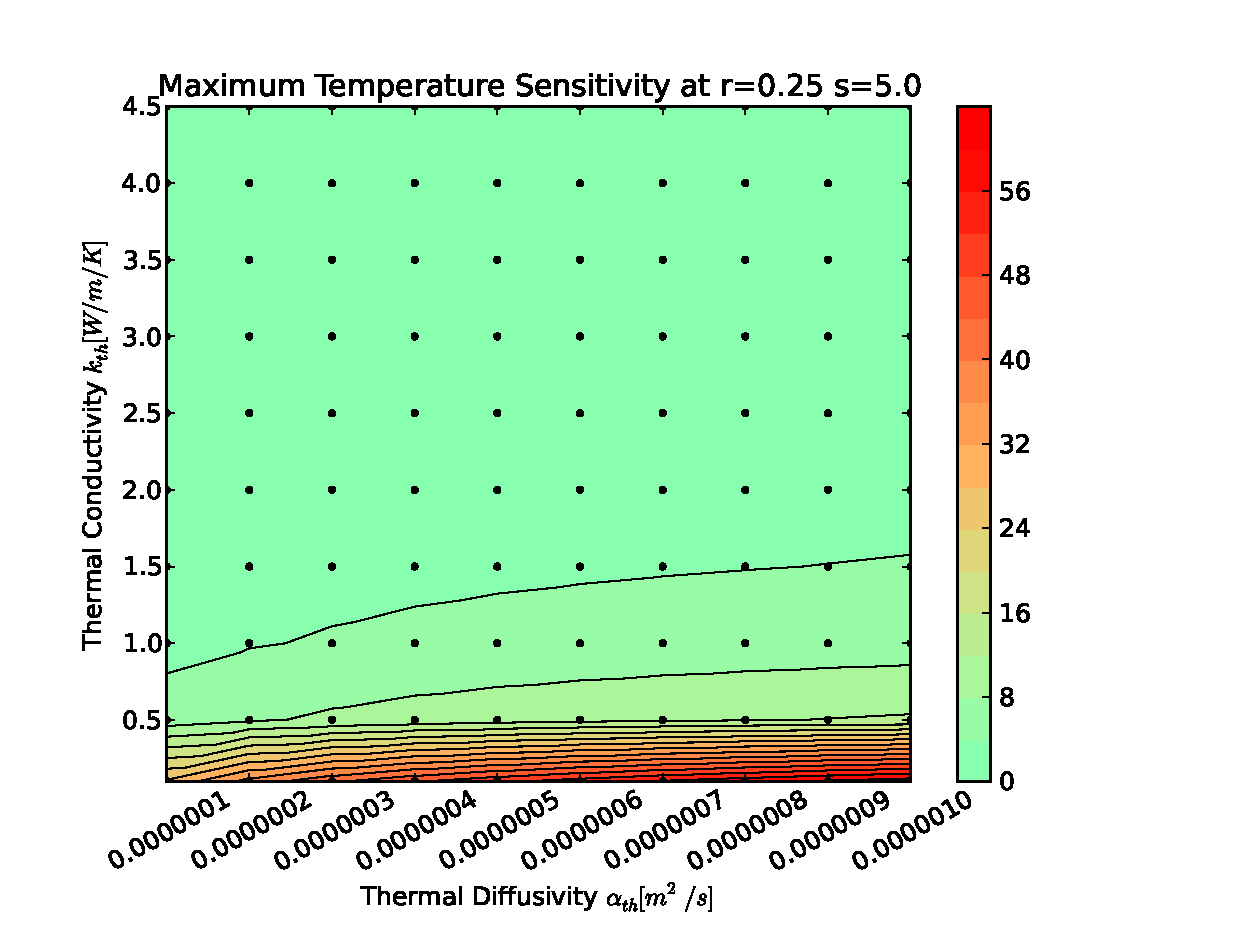
\includegraphics[width=0.7\textwidth]{./chapters/demonstration/diffusivity/ak.eps}
\end{center}
\caption[$\alpha_{th}$ vs. $K_{th}$ Sensitivity in Cyder]{Cyder trends agree
with those of the LLNL model, in which increased thermal diffusivity results in 
decreased thermal deposition in the near field. The above example thermal 
profile results from 10kg of $^{242}Cm$.} 
\label{fig:ar}
\end{figure}


\begin{figure}[htbp!]
\begin{center}
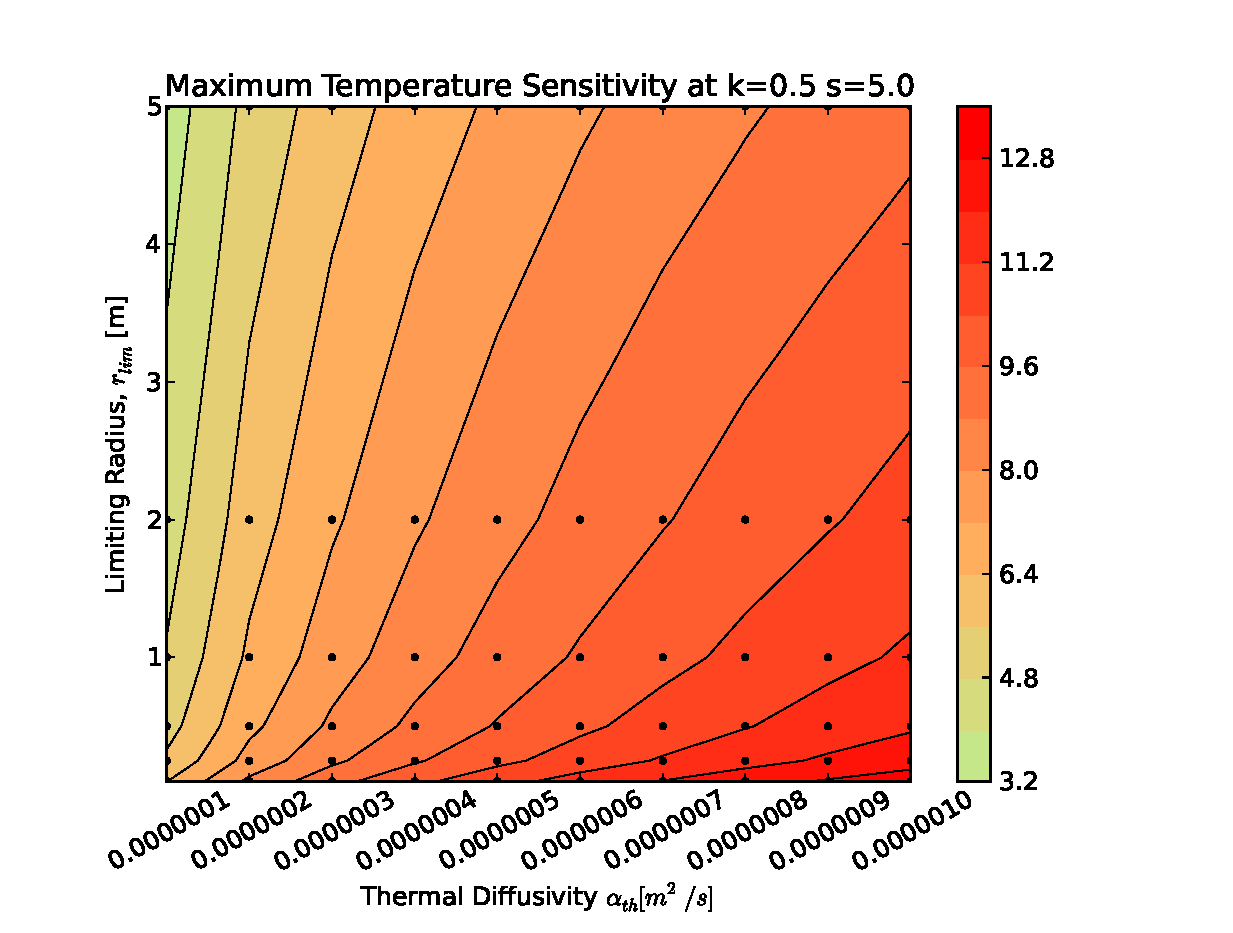
\includegraphics[width=0.7\textwidth]{./chapters/demonstration/diffusivity/ar.eps}
\end{center}
\caption[$\alpha_{th}$ vs. $r_{lim}$ Sensitivity in Cyder]
{Cyder trends agree with 
those of the LLNL model. The importance of the limiting radius decreases with 
increased $K_{th}$. The above example thermal profile results from 10kg of 
$^{242}Cm$}
\label{fig:ak}
\end{figure}

\subsection{Waste Package Spacing Sensitivity Validation}\label{sec:spacing}
The waste package spacing, $s$ of geologic repository concept affects the areal 
decay heat burden in the repository and has a strong effect on the thermal 
energy deposited per unit area in the medium. 

\FloatBarrier
\subsubsection{LLNL Model Results}

In the creation of the \gls{STC} database, the waste package spacing was varied 
across a number of values for each isotope, $i$, limiting 
radius $r_{calc}$, thermal diffusivity $\alpha_{th}$, and thermal conductivity $K_{th}$, considered.  By 
varying the waste package spacing of the geometric layout from $0.1-5 [m]$
this sensitivity analysis succeeds in capturing the domain of 
waste package spacings present in geologic repository concepts under 
consideration. 

\begin{figure}[htbp!]
\begin{center}
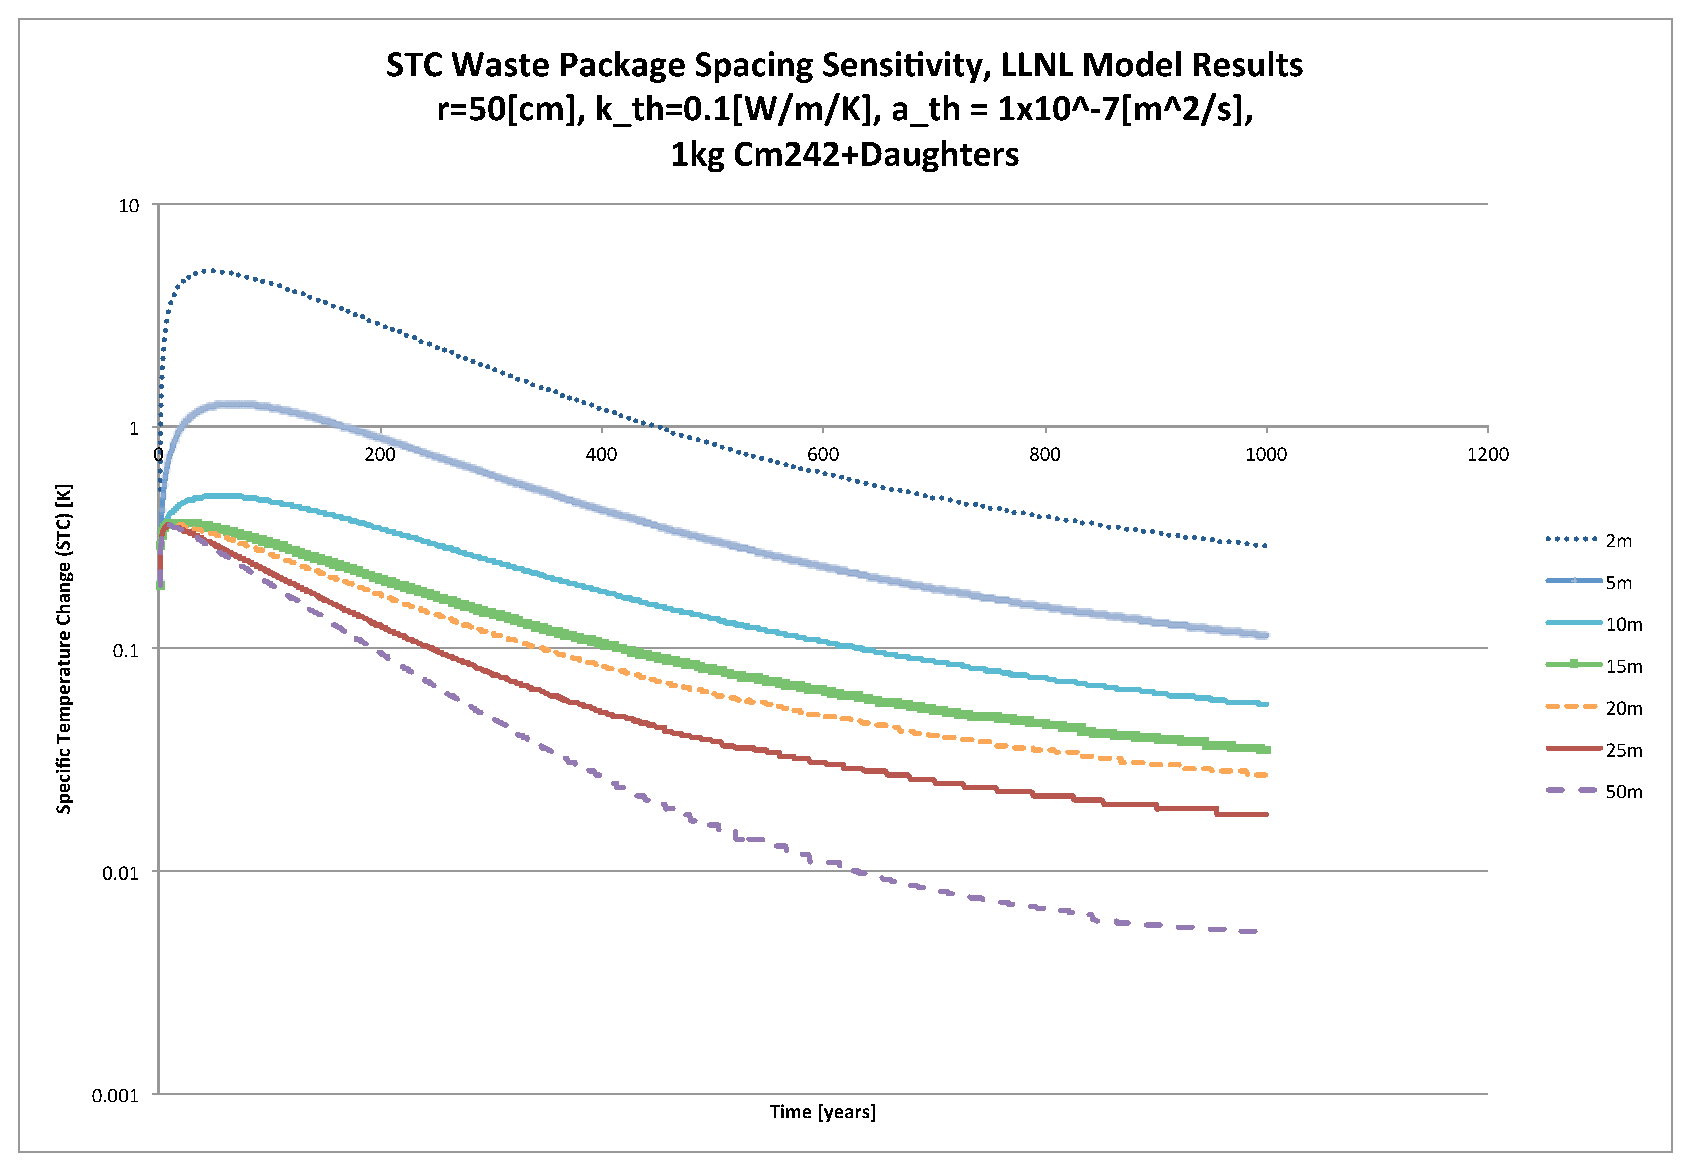
\includegraphics[width=0.7\textwidth]{./chapters/demonstration/spacing/Cm242spacing_sens.eps}
\end{center}
\caption[$K_{th}$ Sensitivity to $s$]{Increased waste package 
spacing decreases areal thermal energy deposition 
(here represented by \gls{STC}) in the near field (here $r_{calc} = 0.5m$).}
\label{fig:Cm242spacing_sens}
\end{figure}

Figure \ref{fig:Cm242spacing_sens} shows the trend in which increased waste package spacing of a medium decreases areal thermal energy 
deposition in the near field. This indicates that waste package spacing is 
an important parameter for repository concept design.

Similarly, the location of the limiting radius has a strong effect on the 
waste package loading limit, for a fixed limiting temperature. In Figure 
\ref{fig:Cm242r_lim_sens}, the trend is demonstrated in which increased limiting 
radius decreases the thermal energy contributing to the thermal limit. 


\begin{figure}[htbp!]
\begin{center}
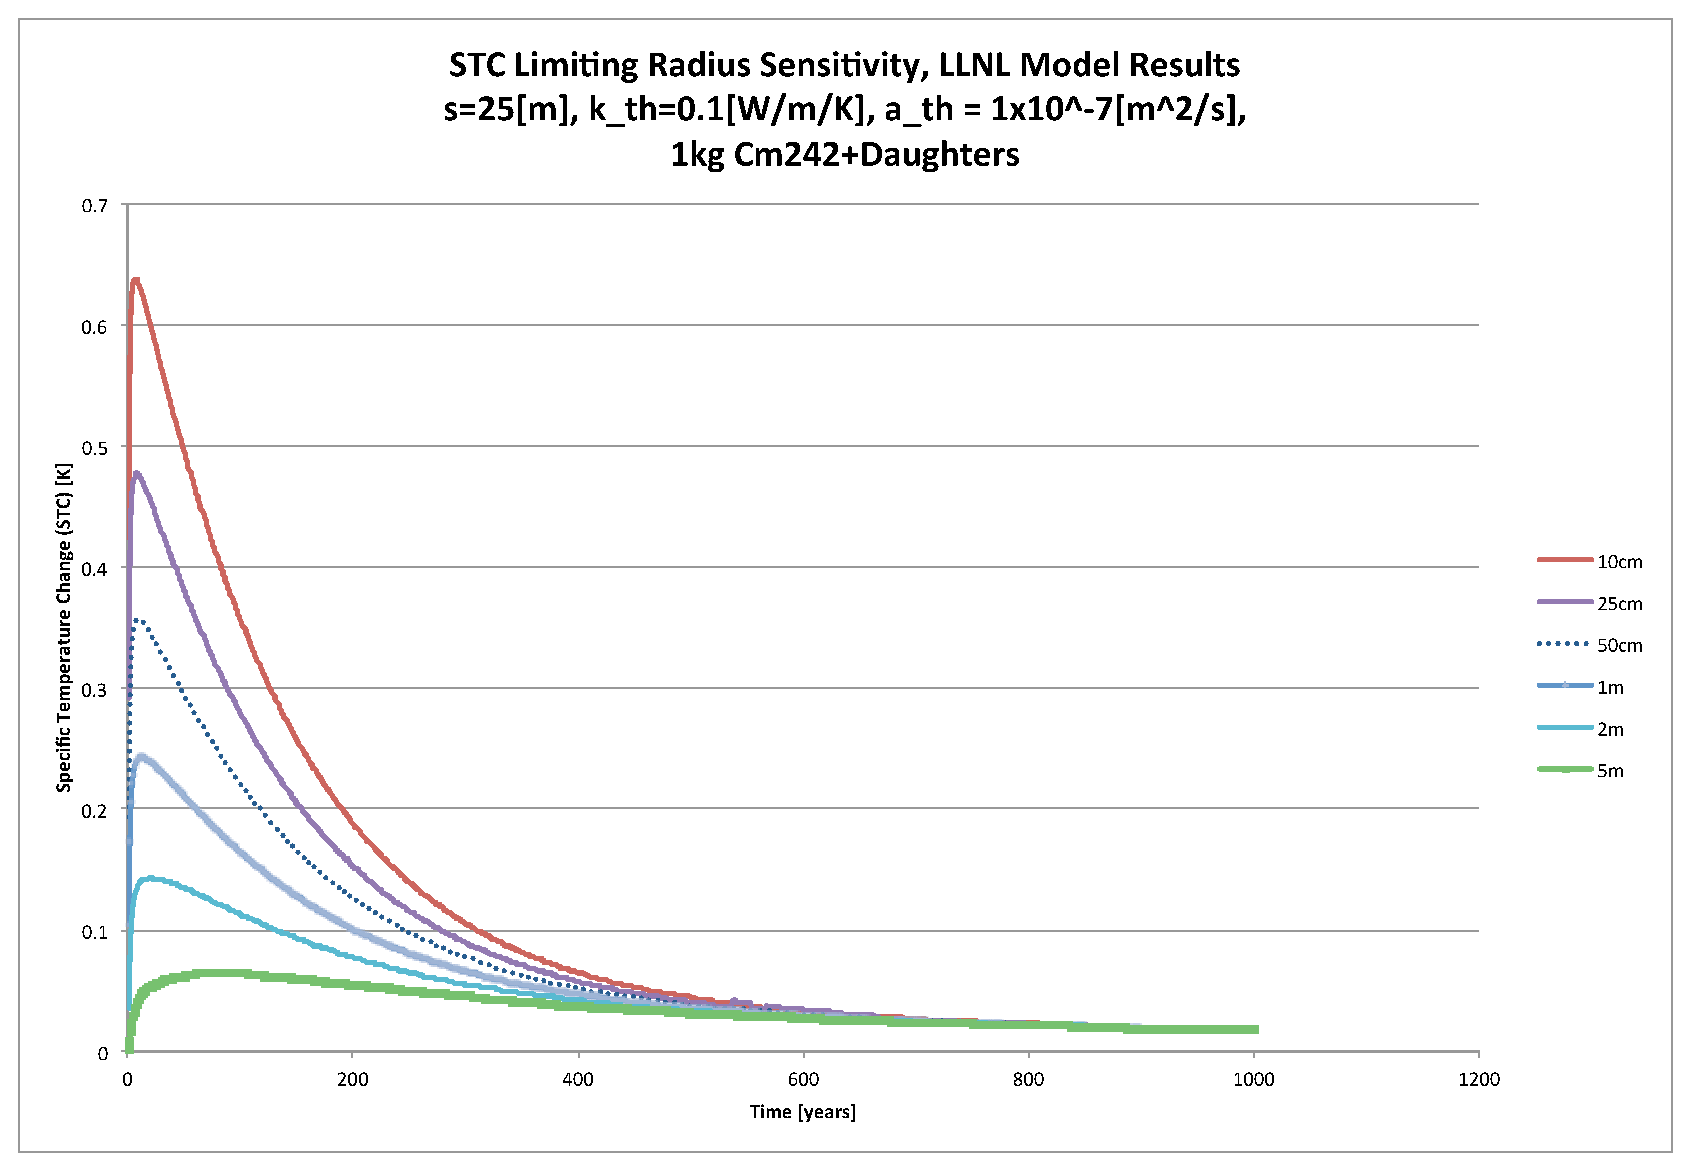
\includegraphics[width=0.7\textwidth]{./chapters/demonstration/spacing/Cm242r_lim_sens.eps}
\end{center}
\caption[$K_{th}$ Sensitivity to $r_{lim}$]{Increased limiting radius 
decreases thermal energy deposition contributing to the thermal limit
(here represented by \gls{STC}).}
\label{fig:Cm242r_lim_sens}
\end{figure}


\FloatBarrier
\subsubsection{Cyder Results}

In a similar analysis, the thermal diffusivity was compared both with the 
spacing between waste packages and the limiting radius. 

Figure \ref{fig:rs} validates the trend noted above that 
increased waste package spacing in a repository concept decreases areal thermal energy deposition 
in the near field.  Additionally, analysis with the \Cyder STC database 
demonstrates the way in which the importance of $r_{lim}$, the limiting radius, 
impacts the maximum calculated temperature at that radius. 


\begin{figure}[htbp!]
\begin{center}
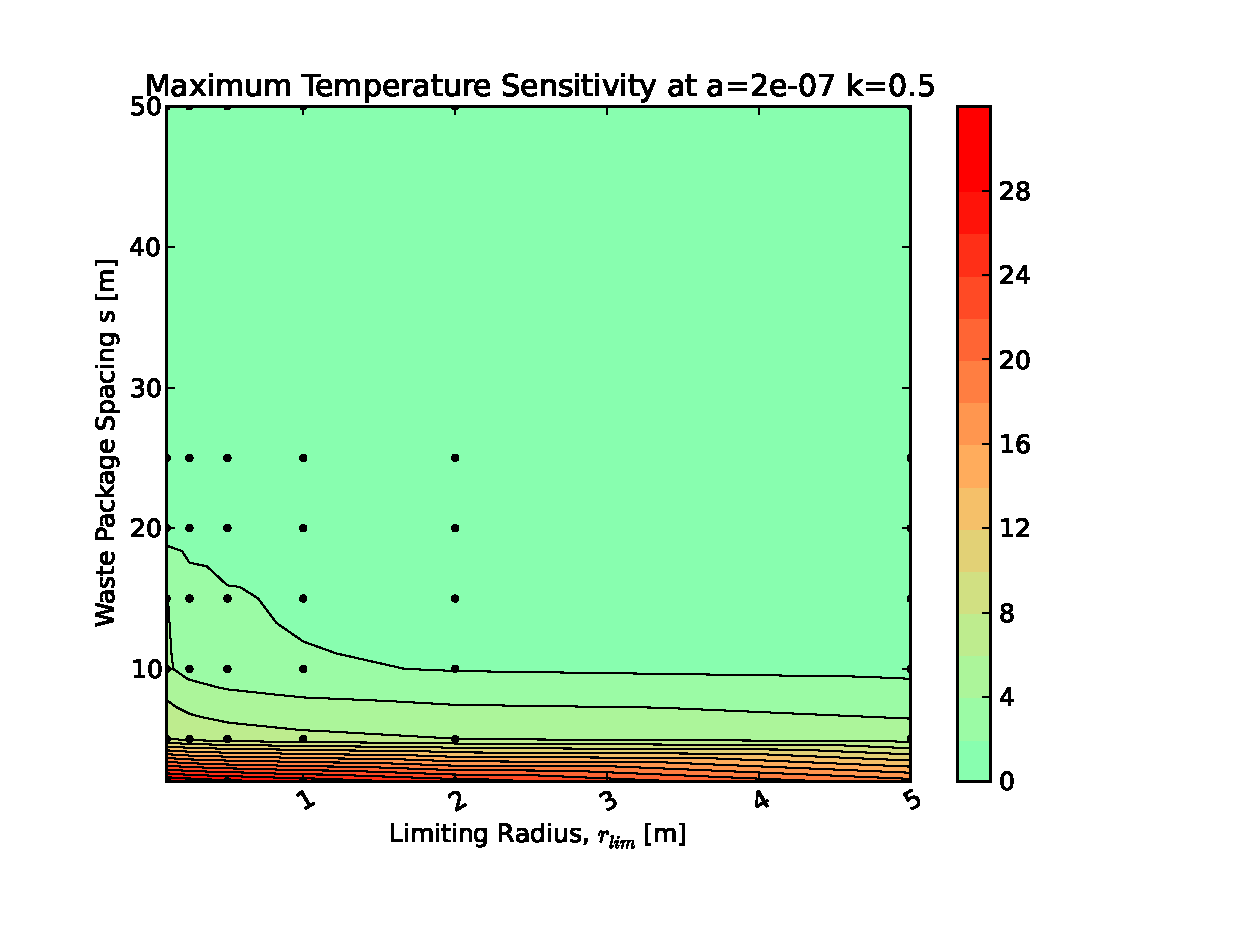
\includegraphics[width=0.7\textwidth]{./chapters/demonstration/spacing/rs.eps}
\end{center}
\caption[$\alpha_{th}$ vs. $r_{lim}$ Sensitivity in Cyder]
{Cyder results agree with 
those of the LLNL model. The importance of the limiting radius decreases with 
increased $K_{th}$. The above example thermal profile results from 10kg of 
$^{242}Cm$}
\label{fig:rs}
\end{figure}



\section{Radionuclide Mass Transfer In \textsc{Cyder}}\label{sec:nuclide_models}

The results here provide an overview of the relative importance of thermal
parameters that affect the repository capacity of simplified generic
disposal concept in various geologic media where conduction is the dominant
heat transfer mode. The applicability of this sensitivity analysis is thus
restricted to enclosed, backfilled concepts.  

\subsection{Parametric Domain}

Sensitivity analyses were conducted which span the parametric range of values 
generated by the reference specific temperature change database and described 
in Table \ref{tab:thermal_cases}.  

\begin{table}[ht!]
\centering
\footnotesize{
\begin{tabular}{|l|l|l|r|}
\multicolumn{4}{c}{\textbf{Thermal Cases}}\\
\hline
\textbf{Parameter} & \textbf{Symbol} & \textbf{Units} & \textbf{Value Range} \\
\hline
Diffusivity & $\alpha_{th}$ & $[m^2\cdot s^{-1}]$ & $1.0\times10^{-7}-3.0\times10^{-6}$\\
\hline
Conductivity & $K_{th}$     & $[W\cdot m^{-1} \cdot K^{-1}]$ & $0.1 - 4.5$ \\
\hline
Spacing & $S$ & $[m]$ & 2, 5, 10, 15, 20, 25, 50 \\
\hline
Radius & $r_{lim}$ & $[m]$ & 0.1, 0.25, 0.5, 1, 2, 5 \\
\hline
Isotope & $i$ & $[-]$ & $^{241,243}Am,$  \\
        & & & $^{242,243,244,245,246}Cm,$  \\
        & & & $^{238,240,241,242}Pu$  \\
        & & & $^{134,135,137}Cs$  \\
        & & & $^{90}Sr$  \\
\hline
\end{tabular}
\caption{A thermal reference dataset of \gls{STC} values as a function of each of these parameters was generated by repeated parameterized runs of the LLNL 
MathCAD model\cite{greenberg_application_2012, greenberg_investigations_2012}.}
\label{tab:thermal_cases}
}
\end{table}



These values were selected to provide detail in the near field and at values of
$\alpha_{th}$ and $K_{th}$ in the three host media under consideration in this
work.

\subsection{Approach}

% used existing gdsms 
This analysis utilized the \gls{LLNL} semi-analytic MathCAD model
discussed in Section \ref{sec:llnl_background}.  It performs detailed
calculations of the conductive thermal transport in a generic repository
concept with a gridded layout.  

It relies on the thermal diffusivity, $\alpha_{th}$ and conductivity $K_{th}$ of 
the material as well as the waste package spacing, $S$, and thermally limiting 
radius, $r_{lim}$. Finally, it relies on the \gls{STC} data calculated with the 
semi-analytic model based on the decay heat profiles of the emplaced wastes, $Q$. 
The essential decay heat profiles, $Q$, were retrieved from a \gls{UFD} database 
provided by Carter et al. \cite{carter_fuel_2011}.




%\subsection{Mass Transfer Modes}\label{sec:mass_transfer}

\subsubsection{Calculation of Mass Transfer}
The MixedCell model can operate in four modes, each dictating the method by 
which mass transfer across the inner boundary is calculated.  Those modes 
utilize the source term, Dirichlet, and Neumann interfaces to model prescribed, 
flow, advective flow, or diffusive flow.
Once calculated, that material object is removed from the 
internal component ($m_{ij} = -\dot{m}_i$) such that its internal state can be 
queried accurately in future timesteps.  

For the case in which source term is used on the inner boundary, the mass 
transferred from component $i$ to component $j$ in timestep $t_{n}$ is simply

\begin{align} 
m_{ij} &=  \mathcal{S}_i(t_n) \nonumber
\intertext{where}
\mathcal{S}_i(t_n) &= \mbox{ source term provided by component i at }t_n [kg].
\end{align}

For the case in which Dirichlet is used, the mass transferred is determined by 
advection. One dimensional mass flux due to advection is the speed of flowing 
water, $v_z$, scaled by the concentration of contaminants fixed by the Dirichlet 
boundary condition, $C$, all integrated over the porous, degraded area perpendicular to 
the flow, $\theta dxdy$,

\begin{align}
  m_{ij} &= \int_{t_{n-1}}^{t_n}\int_0^y\int_0^x\theta d v_z \mathcal{D}_i(t_n) dxdydt \label{mixed_adv}
\intertext{which, for the Cyder components, becomes }
m_{ij} &= \theta d v_z C 2rl (t_n - t_{n-1})\nonumber\\
\intertext{where}
\mathcal{D}_i(t_n) &= \mbox{ fixed C from component i at }t_n [kg/m^3]\nonumber\\
r &= \mbox{ radius of the cylinder }[m]\nonumber\\
l &= \mbox{ length of the cylinder }[m].\nonumber
\end{align}

For the case in which Neumann is chosen, the mass transfer is taken to be 
dispersive, 

\begin{align}
  m_{ij} &= \int_{t_{n-1}}^{t_n}\int_0^y\int_0^x -D \theta d \mathcal{N}_i(t_n) dxdydt \label{mixed_adv}\\
         &= \int_{t_{n-1}}^{t_n}\int_0^y\int_0^x -D \theta d \frac{\partial C}{\partial z}\Bigg|_{z=r_j} dxdydt \nonumber
\intertext{which, for the Cyder components, becomes }
m_{ij} &= -D \theta d \frac{\partial C}{\partial z}\Bigg|_{z=r_j} 2rl(t_n - t_{n-1}).\nonumber
\end{align}

\subsubsection{Boundary Interfaces}
The source term of available contaminants is all mass in the available degraded fluid,
\begin{align}
\mathcal{S}_j(t_n) &= m_{df}(t_n). 
\end{align}
The desired boundary conditions can be expressed in terms of $m_{df}$. First, the 
Dirichlet boundary condition is 
\begin{align}
\mathcal{D}_j(t_n) &= C_j(t_n)\nonumber\\ 
 &= \frac{m_{df}(t_n)}{V_{df}(t_n)}.
\label{dirichlet_mixed}
\end{align}

From this boundary condition in combination with global advective velocity 
data, porosity data,  and elemental dispersion coefficient data, all other 
boundary conditions can be found. The Neumann boundary condition generated at 
the external boundary of cell $j$ relies on up to date data from cell $k$ and 
on internal state data from the previous time step, such that 

\begin{align}
\mathcal{N}_j(t_n)&= \frac{dC(t_n)}{dr}\Bigg|_{r=r_j}\nonumber\\ 
                  &= \frac{C_k(r_{k-1/2},t_{n-1}) - C_i(r_{j-1/2}, t_n)}{r_{k-1/2} - r_{j-1/2}}
\label{neumann_mixed}
\intertext{where}
r_{j-1/2} &= r_{j} - \frac{r_{j} - r_{i}}{2}.\nonumber\\
r_{k-1/2} &= r_{k} - \frac{r_{k} - r_{j}}{2}.\nonumber
\end{align}

This expression for the concentration gradient can also be used in the Cauchy 
boundary condition, which relies on the advective velocity and concentration 
profile as well as the concentration gradient,

\begin{align}
v_z C_0 &= \frac{dC(t_n)}{dr}\Big|_{r=r_{j}} + v_{z}C_j(t_n).
\label{cauchy_mixed}
\end{align}


%\subsection{Time Step Algorithm}\label{sec:timestep}
\subsection{Time Stepping Algorithm}\label{sec:time stepping}

In \Cyder, radionuclide contaminant flow is assumed to travel outward from 
the central Component (and up, in the $\hat{k}$ direction). In order to conduct 
a mass balance in each Component at each time step, the mass flow and mass 
balance calculations proceed from the innermost Component to the outermost 
Component. As mass flows from inner components to outer components, the mass 
balances in both components are updated.  Thus, nuclide release information is 
passed radially outward from the waste stream sequentially through each 
containment layer to the geosphere.  This implicit time stepping method 
arrives at the updated state of each Component, radially outward, as a function 
of both the past state and the current state of the system. 

At each component interface where mass transfer occurs and within each component 
where mass balances take place, the flow model is solved with the most up to 
date information available.  To illustrate the algorithm by which mass flow 
calculations are conducted through the system of components at each time step, we 
will walk through the phases of a single time step for a simple pair of 
components. The source, $i$, is the inner and the sink, $j$, is the outer
component. 

\subsubsection{Phase 1: Initial Conditions}

The initial conditions in both the source and the sink at the beginning of a 
time step are equal to the final updated state of the previous time step. If this 
is the first time step, the global intial state of the repository system is used. 

\subsubsection{Phase 2: Interior Mass Balance}

The mass distrubution and concentration profile in the interior source volume 
$i$ is solved based on the initial condition, any influxes, and the physics of 
its mass balance model.  This calculation results in a contaminant mass 
distribution and concentration profile within the volume $i$ at time $t_n$.  
For each of the models, the calculation behind this mass distribution and 
concentration profile is disscussed in Section \ref{sec:mass_balance}.

This mass distribution and concentration profile fully inform 
the conditions on the boundary at $r_i$ and this information is made available 
to the external component, $j$.


\subsubsection{Phase 3: Mass Transfer Calculation}

The mass transfer from the source volume $i$ to the sink volume $j$ is 
calculated next, based on the up to date conditions at $0\le r \le r_{i}$ 
determined in Phase 2 and the initial conditions in volume $j$ where $r_i \le r 
\le r_j$. The mass transfer is calculated according to the mass transfer mode 
preference of the mass balance model of volume $j$.  

The Degradation Rate and Mixed Cell models can be parameterized to utilize an 
explicit mass transfer mode that captures either advection, dispersion, or 
coupled flow.  The Lumped Parameter and One Dimensional PPM models, on the 
other hand, use an implcit method by which the incoming mass flux is determined 
based on the expected concentration profile resulting from the internal 
Dirichlet boundary condition at $r_i$. 

\subsubsection{Phase 4: Exterior Mass Balance}

When a mass flux $m_{ij}(t_n)$ is determined between volumes $i$ and $j$, the 
mass is added to the exterior sink volume $j$. Accordingly, necessary updates 
are made to the mass balance and concentration profile.  For each of the 
models, the calculation behind this mass distribution and concentration profile 
is disscussed in Section \ref{sec:mass_balance}.

\subsubsection{Phase 5: Interior Mass Balance Update}

When a mass flux $m_{ij}(t_n)$ is determined between volumes $i$ and $j$, the 
mass is simultanously added to the exterior sink volume $j$ (as in phase 4) and 
extracted from the interior source volume $i$.  When the material is extracted 
from the interior source volume, the contained mass distribution and 
concentration profile are updated to reflect this change.  

\subsubsection{old text}


That is, in Component $j$, some Component in a nested series, the mass flux 
entering the Component at time $t_n$ is found from the initial state of the cell 
at time $t_n$, the inner boundary 
condition at time $t_n$ and the outer boundary condition at $t_{n-1}$.  

\begin{align}
  \dot{m}_{ij}^n &= f( m_j(t_{n-1}) , BC_i(t_n) , BC_j(t_{n-1}) . . . ) \nonumber\\
  \intertext{where}
  m_{ij}(t_n) &= \mbox{ contaminant mass flux from component i to j }[kg/time step]\nonumber\\
  BC_i(t_n)  &= \mbox{ inner conditions at }r_i\mbox{, and time }t_n \nonumber \\
  BC_j(t_{n-1})  &= \mbox{ outer conditions at }r_j\mbox{, and time }t_{n-1} \nonumber\\
  f &= \mbox{ functional form of contaminant transport into j. }\nonumber
\end{align}

Once the mass flux into the component is found, the mass is removed from the 
inner cell, updating its state in preparation for the next time step.

\begin{align}
  m_i^\dagger(t_n)  &= m_i(t_n)  - m_{ij}(t_n) 
  \intertext{where}
  m_i^\dagger(t_n)  &= \mbox{ updated mass in component i }[kg]
\end{align}

In this way, the contained mass in the component is described as
\begin{align}
  m_j(t_n)  &= m_j(t_{n-1})  + \dot{m}_j(t_n) . \nonumber
\end{align}

Resulting concentration profiles across the component can then be calculated 
and one can solve, numerically, for the outer boundary condition at $t_n$ 

\begin{align}
  BC_j(t_n) &= g\left( m_j(t_n) , C_j(t_n) \right)\nonumber\\
  g &= \mbox{functional form of contaminant transport across j}\nonumber
\end{align}

This boundary condition can, in turn, be used by the component external to it, $k$ as the $t_n$ 
inner boundary condition of its own solution and so on.



%\subsection{Mass Inventory and Distribution Models}\label{sec:mass_balance}

The results here provide an overview of the relative importance of thermal
parameters that affect the repository capacity of simplified generic
disposal concept in various geologic media where conduction is the dominant
heat transfer mode. The applicability of this sensitivity analysis is thus
restricted to enclosed, backfilled concepts.  

\subsection{Parametric Domain}

Sensitivity analyses were conducted which span the parametric range of values 
generated by the reference specific temperature change database and described 
in Table \ref{tab:thermal_cases}.  

\begin{table}[ht!]
\centering
\footnotesize{
\begin{tabular}{|l|l|l|r|}
\multicolumn{4}{c}{\textbf{Thermal Cases}}\\
\hline
\textbf{Parameter} & \textbf{Symbol} & \textbf{Units} & \textbf{Value Range} \\
\hline
Diffusivity & $\alpha_{th}$ & $[m^2\cdot s^{-1}]$ & $1.0\times10^{-7}-3.0\times10^{-6}$\\
\hline
Conductivity & $K_{th}$     & $[W\cdot m^{-1} \cdot K^{-1}]$ & $0.1 - 4.5$ \\
\hline
Spacing & $S$ & $[m]$ & 2, 5, 10, 15, 20, 25, 50 \\
\hline
Radius & $r_{lim}$ & $[m]$ & 0.1, 0.25, 0.5, 1, 2, 5 \\
\hline
Isotope & $i$ & $[-]$ & $^{241,243}Am,$  \\
        & & & $^{242,243,244,245,246}Cm,$  \\
        & & & $^{238,240,241,242}Pu$  \\
        & & & $^{134,135,137}Cs$  \\
        & & & $^{90}Sr$  \\
\hline
\end{tabular}
\caption{A thermal reference dataset of \gls{STC} values as a function of each of these parameters was generated by repeated parameterized runs of the LLNL 
MathCAD model\cite{greenberg_application_2012, greenberg_investigations_2012}.}
\label{tab:thermal_cases}
}
\end{table}



These values were selected to provide detail in the near field and at values of
$\alpha_{th}$ and $K_{th}$ in the three host media under consideration in this
work.

\subsection{Approach}

% used existing gdsms 
This analysis utilized the \gls{LLNL} semi-analytic MathCAD model
discussed in Section \ref{sec:llnl_background}.  It performs detailed
calculations of the conductive thermal transport in a generic repository
concept with a gridded layout.  

It relies on the thermal diffusivity, $\alpha_{th}$ and conductivity $K_{th}$ of 
the material as well as the waste package spacing, $S$, and thermally limiting 
radius, $r_{lim}$. Finally, it relies on the \gls{STC} data calculated with the 
semi-analytic model based on the decay heat profiles of the emplaced wastes, $Q$. 
The essential decay heat profiles, $Q$, were retrieved from a \gls{UFD} database 
provided by Carter et al. \cite{carter_fuel_2011}.



%\subsubsection{Degradation Rate Mass Balance Model}\label{sec:deg_rate}
\subsection{Degradation Rate Radionuclide Transport Model}\label{sec:deg_rate}
The degradation rate model, simulating the fractional degradation of the 
material containment properties, is the simplest of implemented models and is most 
appropriate for simplistic waste package failure modeling. The fundamental 
concept is depicted in Figure \ref{fig:deg_volumes}.

\begin{figure}[h!]
  \begin{center}
    \def\svgwidth{.7\textwidth}
    \input{./chapters/methodology/nuclide_models/mass_balance/deg_rate/deg_volumes.eps_tex}
  \end{center}
  \caption[Constituents of a Degradation Rate Control Volume]{The control volume contains an 
  intact volume $V_i$ and a degraded volume, $V_d$. Contaminants in $V_d$ are 
  available for transport, while contaminants in $V_i$ are contained.}
  \label{fig:deg_volumes}
\end{figure}



The materials that constitute the engineered barriers in a saturated 
repository environment degrade over time. The implemented model of this nuclide 
release behavior is based solely on a fractional degradation rate. 
The degraded volume is a simple fraction, $d$, of the total volume, $V_T$, such 
that 
\begin{align}
V_T &= V_i + V_d
\label{deg_volumes}
\intertext{where}
V_d(t) &= d(t)V_T\nonumber\\
V_i(t) &= (1-d(t))V_T\nonumber\\
V_T &= \mbox{ total volume }[m^3]\nonumber\\
V_i(t) &= \mbox{ intact volume at time t }[m^3]\nonumber\\
V_d(t) &= \mbox{ degraded volume at time t }[m^3]\nonumber
\intertext{and}
d(t) &= \mbox{ the fraction that has been degraded by time t }[-].\nonumber
\end{align}


\subsubsection{Calculation of Mass Transfer}
In this model, the contaminants in the degraded fraction of the control volume 
are available to adjacent components. The available contaminants
$m_{ij}(t)$, at the boundary between cell $i$ to cell $j$ at time $t$ are thus

\begin{align}
\dot{m}_{ij}(t) &= f_im_i(t)
\label{deg_rate_source_cont}
\intertext{where}
\dot{m}_{ij} &= \mbox{ the rate of mass transfer from i to j }[kg/s]\nonumber\\
f_i &= \mbox{ degradation rate function in cell i }[1/s] \nonumber\\
m_i &= \mbox{ mass in cell i }[kg] \nonumber\\
t &= \mbox{ time  }[s].\nonumber
\end{align}

For a situation as in \Cyder and \Cyclus, with discrete time steps, the time steps are 
assumed to be small enough to assume a constant rate $m_{ij}$ over the course 
of the time step. This model incorporates the source term made available on the 
inner boundary into its available mass and defines the resulting boundary 
conditions at the outer boundary as solely a function of the degradation rate 
of that component.  The mass transferred between discrete times $t_{n-1}$ and 
$t_n$ is thus a simple linear function of the transfer rate in 
\eqref{deg_rate_source_cont}, 

\begin{align}
m_{ij}(t_n) &= \int_{t_{n-1}}^{t_n}\dot{m}_{ij}(t')dt' \nonumber\\
         &= f_im_i(t_{n-1})\left[t_n - t_{n-1}\right].
\label{deg_rate_source_discrete}
\end{align}

\subsubsection{Boundary Interfaces}
\label{sec:dr_bc}
The mass $m_{df}(t_n)$ is the source term at the outer boundary, 
\begin{align}
  \mathcal{S}_j(t_n) &= \mbox{ fixed source term flux at }r_j [kg]\nonumber\\ 
                     &= m_{df}(t_n).
\end{align}
Thus, for the case in which all engineered barrier components are represented by 
degradation rate models, the source term at the outermost edge will be solely
a function of the original central source and the degradation rates of the 
components. 

The concentration boundary condition must also be defined at the outer boundary 
to support parent components that utilize the Dirichlet boundary condition. For 
the degradation rate model, which incorporates no diffusion or advection, the 
concentration, $C_j$ at $r_j$, the boundary between cells $j$ and $k$, is the average 
concentration in the saturated pore volume,

\begin{align}
\mathcal{D}_j(t_n) &= \mbox{ fixed concentration from component j at }t_n [kg/m^3].\nonumber\\ 
                   &= C_{j}(t_n)\nonumber\\ 
                   &= C_{df}\nonumber\\
                   &= \frac{m_{d}(t_n)}{V_{d}(t_n)}\\
\label{deg_rate_dirichlet}\\
&= \frac{\mbox{ solute mass in degraded fluid in cell j }}{\mbox{ degraded fluid volume in cell j}}.\nonumber 
\end{align}

To support parent components that utilize the Neumann boundary condition, the 
concentration gradient can be found if the concentration and the 
radial midpoint of the external component, $k$, are specified.

\begin{align}
\mathcal{N}_j(t_n) &= \mbox{ fixed concentration gradient from component j at }t_n [kg/m^3/s]\nonumber\\
                   &= \frac{dC(t_n)}{dr}\Bigg|_{r=r_j}\nonumber\\ 
                   &= \frac{C_k(r_{k-1/2},t_{n-1}) - C_j(r_{j-1/2}, t_n)}{r_{k-1/2} - r_{j-1/2}}
\label{neumann_dr}
\intertext{where}
r_{j-1/2} &= r_{j} - \frac{r_{j} - r_i}{2}\nonumber\\
r_{k-1/2} &= r_{k} - \frac{r_{k} - r_j}{2}.\nonumber
\end{align}


To support parent components that utilize the Cauchy boundary condition, the 
degradation rate model assumes that the fluid velocity is constant across the cell 
as is the concentration. Thus, 

\begin{align}
\mathcal{C}_j(t_n) &= \mbox{ fixed concentration flux from component j at }t_n [kg/m^2/s]\nonumber\\
                   &= -D\frac{\partial C(t_n)}{\partial r}\Bigg|_{r=r_j} + v_zC(t_n)\Bigg|_{r=r_j} \\
\label{deg_rate_cauchy}
            &= v_zC_0\nonumber
\intertext{where}
            C_0 &= \mbox{ a fixed concentration }[kg/m^3].\nonumber
\end{align}

%<++> &= \mbox{ <++> }[<++>] \nonumber\\


%\subsubsection{Mixed Cell Mass Balance Model}\label{sec:mixed_cell}
\section{Mixed Cell Volume Radionuclide Model}\label{sec:mixed_cell}

    % WF : glass 

      % alteration

      % temperature limit

    % WF : uox 

      % cladding limit

      % corrosion

A main nuclide transport component model used in this work is a mixed cell 
component module incorporating solubility and sorption effects as well as  
engineered material dissolution.

A graphical representation of the mixed cell model is given in Figures 
\ref{fig:intact} and \ref{fig:dissolved}.  

\begin{figure}[h!]
\begin{minipage}[b]{0.5\linewidth}
  \begin{center}
    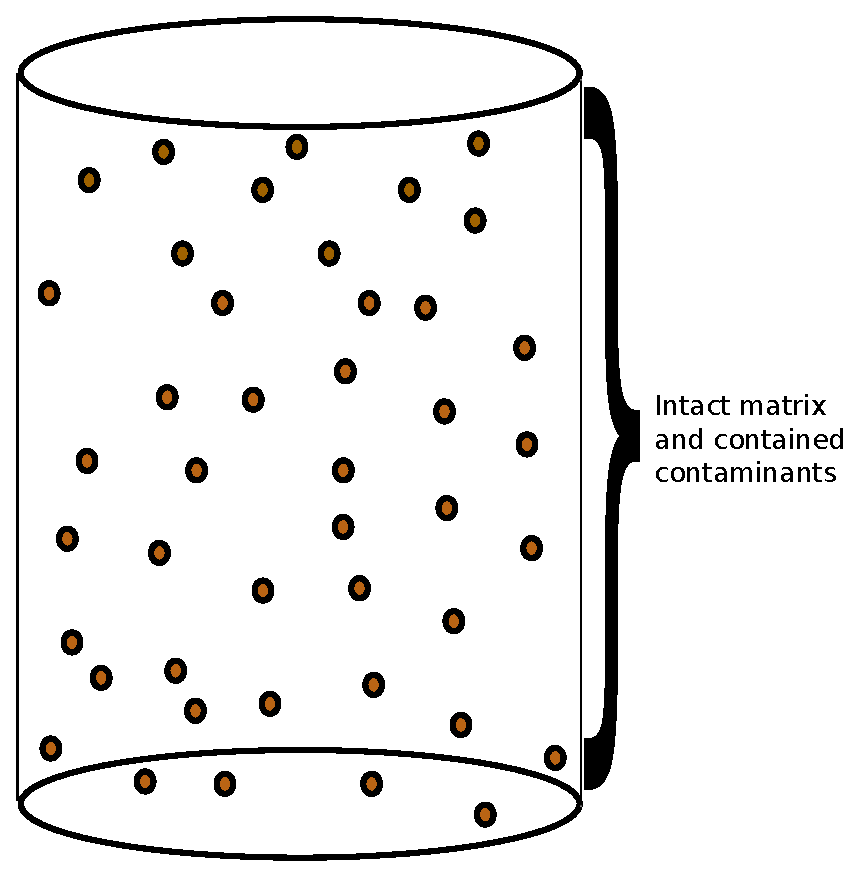
\includegraphics[height=7cm]{./chapters/nuclide_models/mixed_cell/mixed_cell_whole.eps}
  \end{center}
  \caption[Intact Mixed Cell Control Volume]{The control volume contains an 
  intact material matrix and contaminants that are unavailable to neighboring 
  subcomponents until dissolution has begun.}
  \label{fig:intact}
\end{minipage}
\hspace{0.5cm}
\begin{minipage}[b]{0.5\linewidth}
  \begin{center}
    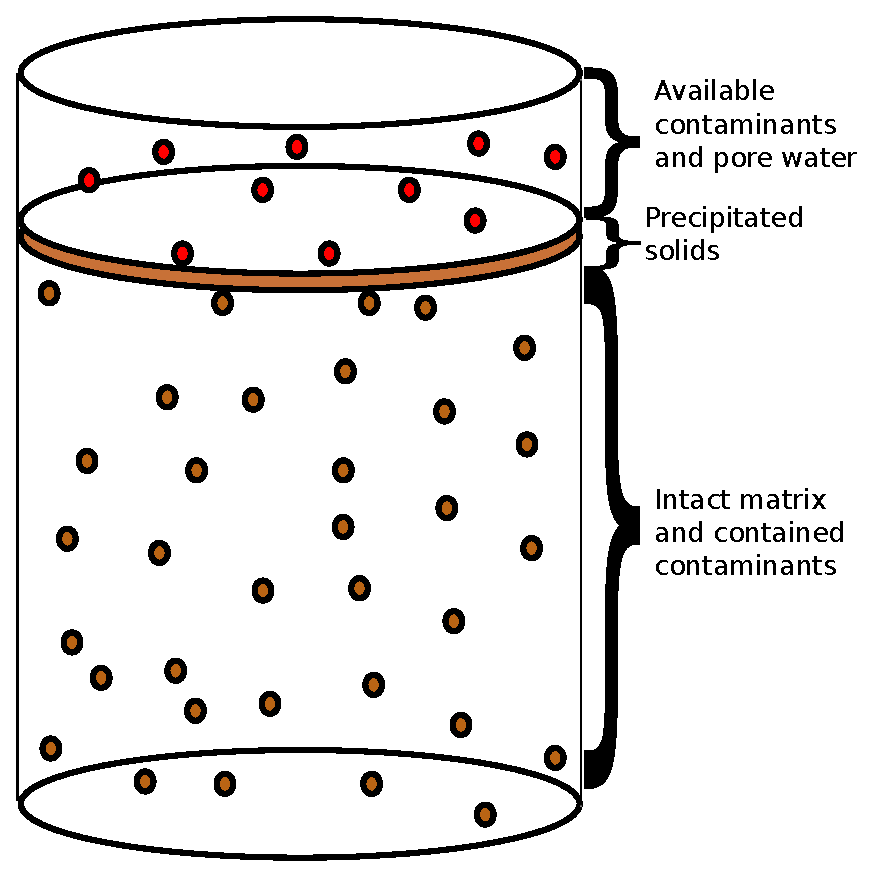
\includegraphics[height=7cm]{./chapters/nuclide_models/mixed_cell/mixed_cell_degraded.eps}
  \end{center}
  \caption[Degrading Mixed Cell Control Volume]{Once dissolution begins, the 
  :control volume contains a partially dissolved material matrix, contaminated 
  pore water, and precipitated solids.}
  \label{fig:dissolved}
\end{minipage}
\end{figure}


After some time degrading, the volume of free fluid can be expressed 
\begin{align}
V_{ff}(t_n) &= \theta V_T \int_{t_0}^{t_n} f(\cdots) dt.
\label{vff}
\end{align}

The volume of the intact matrix can be expressed
\begin{align}
V_{im}(t_n) &= V_T - V_T\int_{t_0}^{t_n} f(\cdots) dt.
\label{vim}
\end{align}

Finally, the volume of the precipitated solids can be expressed
\begin{align}
V_{ps}(t_n) &= (1 - \theta)V_T\int_{t_0}^{t_n} f(\cdots) dt.
\label{vps}
\end{align}

This model assumes that all net influx to the cell enters the free fluid rather 
than the intact matrix. The total volumetric contaminant concentration in the intact matrix, 
can be expressed

\begin{align}
C_{im}(t_n) &= C_0\\
            &= \frac{m_0}{V_{im}}
\intertext{where}
%here we assume nothing escapes an intact matrix
m_0 &= \mbox{ total initial mass } \nonumber
\end{align}

The resulting contaminant mass in the intact matrix is 

\begin{align}
m_{im}(t_n) &= C_0 V_{im}(t_n)\nonumber\\
            &= C_0(1-\theta) V_T\int_{t_0}^{t_n}f(\cdots)dt. 
\label{mim}
\end{align}

The contaminant mass in the free fluid is just the pore water concentration 
times the free fluid volume plus the time integral of net influx to the cell. 

\begin{align}
C_{ffT}(t_n) &= \left[C_0 + \frac{\int_{t_0}^{t_n} \dot{m}_{i}(t') dt'}{V_{ff}(t_n)}\right] 
\intertext{and}
m_{ffT}(t_n) &= C_{ff}(t_n)\theta V_{ff}(t_n)\nonumber\\
       &= \left[C_0 + \frac{\int_{t_0}^{t_n} \dot{m}_{i}(t') dt'}{V_{ff}(t_n)}\right] V_{ff}(t_n) \nonumber\\
       &= C_0V_{ff}(t_n) + \int_{t_0}^{t_n} \dot{m}_{i} dt'
\end{align}

It is limited, however, by both solubility limitation and sorption. 

\subsection{Sorption}

The mass in both the free fluid and in the intact matrix exists in both 
sorbed and nonsorbed phases. The relationship between the sorbed mass 
concentration in the solid phase (e.g. the pore walls),

\begin{align}
s &=\frac{\mbox{ mass of sorbed contaminant} }{ \mbox{mass of total solid phase }}
\label{solid_conc}
\end{align}
and the dissolved liquid concentration, 
\begin{align}
c &=\frac{\mbox{ mass of dissolved contaminant} }{ \mbox{volume of total liquid phase }}
\label{liquid_conc}
\end{align}
can be expressed by a number of isotherm models.

In this model, sorption is taken into account throughout the volume. In the 
intact matrix, the contaminant mass is distributed between the pore walls and 
the pore fluid by sorption.  So too, contaminant mass released from the intact 
matrix by degradation is distributed between dissolved mass in the free fluid 
and sorbed mass in the precipitated solids.


\subsection{Boundary Conditions}

To solve for the boundary condiitons in this model, the amount of dissolved mass 
in the free fluid must be found. This value, $m_{ffl}$, can be expressed in terms of the 
total degraded contaminant mass and the contaminant mass in the precipitated 
solid,

\begin{align}
m_{ffl} &= m_{ffT} - m_{psc}
\label{m_ffl}
\end{align}

The mass of contaminant sorbed into the precipitated solids can be found using a 
linear isotherm model, characterized by the relationship 
\begin{align}
s_{i} &= K_{di} c_{i}
\label{linear_iso}
\intertext{where}
s_i &= \mbox{ the solid concentration of isotope i }[kg/kg]\nonumber\\
K_{di} &= \mbox{ the distribution coefficient of isotope i}[]\nonumber\\
c_i &= \mbox{ the liquid concentration of isotope i }[kg/m^3].\nonumber
\end{align}

Thus, 

\begin{align}
s_{i,ps} &= \frac{\mbox{contaminant mass in precipitated solids} }{ \mbox{total mass of precipitated solids}}\nonumber\\
         &= \frac{m_{psc}}{m_{pst}}\nonumber\\
         &= \frac{m_{psc}}{m_{psm} + m_{psc}}\nonumber\\
\intertext{where}
m_{psm}  &= \mbox{ noncontaminant mass in precipitated solids }[kg]\nonumber\\
         &= \rho_bV_{ps}\nonumber\\
m_{psc}  &= \mbox{ contaminant mass in precipitated solids }[kg]\nonumber\\
m_{psm}  &= \rho_bV_{ps}.
\label{s_ps}
\end{align}

The following expression results, giving contaminant mass in the precipitated 
solids in terms of the sorption coefficient,
\begin{align}
m_{psc} &= s_{ps}m_{psT}\nonumber\\
          &= K_dC_{ffl}m_{psT}\nonumber\\
          &= \frac{K_dm_{ffl}m_{psT}}{V_{ff}}\nonumber\\
          &= \frac{K_d}{V_{ff}}(m_{ffT}-m_{psc})m_{psT}\nonumber\\
          &= \frac{K_d}{V_{ff}}(m_{ffT}-m_{psc})(m_{psm}+m_{psc})\nonumber\\
          &= \frac{K_d}{V_{ff}}(m_{ffT}m_{psm}-m_{psc}m_{psm} + m_{ff}m_{psc} -m_{psc}^2)\nonumber\\
          &= \frac{K_d}{V_{ff}} (m_{ffT}m_{psm} + (m_{ffT} - m_{psm})m_{psc} - m_{psc}^2)\nonumber
\intertext{which, rearranged, becomes }
0         &= m_{psc}^2 + \left( -m_{ffT} + m_{psm} + \frac{V_{ff}}{K_d} \right)m_{psc} - m_{ffT}m_{psm}\nonumber
\intertext{and is solved using the quadratic formula, such that}
m_{psc}   &= \frac{m_{ffT} - m_{psm} - \frac{V_{ff}}{K_d}}{2} \nonumber\\
          & \pm\frac{\sqrt{m_{ffT}^2 + m_{psm}^2 + \frac{V_{ff}^2}{K_d^2} + 2m_{ffT}m_{psm} - 
             \frac{2V_{ff}m_{ffT}}{K_d} + \frac{2V_{ff}m_{psm}}{K_d} } }{2} \nonumber
\intertext{which, again rearranged, becomes}
          &= \frac{1}{2} \left(m_{ffT} - m_{psm} - \frac{V_{ff}}{K_d}\right) \nonumber\\
          & \pm \frac{1}{2} \sqrt{m_{ffT}^2 + 2m_{ffT}\left(m_{psm} - 
          \frac{V_{ff}}{K_d}\right) + \left(m_{psm} + 
          \frac{V_{ff}}{K_d}\right)^2}.
\label{m_psc}
\end{align}

If we plug Equation \eqref{m_psc} into Equation \eqref{m_ffl}, we arrive at the 
following expression for $m_{ffl}$ in terms of known quantities

\begin{align}
m_{ffl}   &= m_{ffT} - \frac{1}{2} \left(m_{ffT} - m_{psm} - \frac{V_{ff}}{K_d}\right) \nonumber\\
          & \mp \frac{1}{2} \sqrt{m_{ffT}^2 + 2m_{ffT}\left(m_{psm} - 
          \frac{V_{ff}}{K_d}\right) + \left(m_{psm} + 
          \frac{V_{ff}}{K_d}\right)^2}.
\label{m_ffl_full}
\end{align}

We can express the desired boundary conditions in terms of $m_{ffl}$. First, the 
Dirichlet boundary condition is 
\begin{align}
C(x,y,z,t) = \frac{m_{ffl}(t)}{V_{ff}(t)}\forall (x,y,x) \in \Gamma.
\label{dirichlet_mixed}
\end{align}

Again, the concentration gradient can be specified across the boundary only with 
reference to the concentration at a point external to the component. 
If the concentration $C_{ext}$ is specified at a location $r_{ext}$, the Neumann 
condition is a function of those concentrations, $C(x,y,z,t)$, and a 
corresponding location inside the component. If we choose radius furthest from 
either wall of the inner component, $r_c$, 

\begin{align}
\frac{\partial C}{\partial r} = \frac{C_{ext} - C(x,y,z,t)}{r_{ext} - r_{c}}&
\label{neumann_mixed}
\intertext{such that}
\theta_i\vec{v_i}(t) C(x,y,z,t) \frac{C_{ext} - C(x,y,z,t)}{r_{ext} - r_{c}} &= \theta_i\vec{v_i}(t) C(x,y,z,t).
\end{align}





%\subsubsection{Lumped Parameter Mass Balance Model}\label{sec:lumped}
\subsubsection{Lumped Parameter Radionuclide Mass Balance Model}\label{sec:lumped}

For systems in which the flow is sufficiently slow to be assumed constant over 
a time step, it is possible to model a system of volumes as a connected lumped 
parameter models (Figure \ref{fig:lumpedseries}). 
The Lumped Parameter mass balance model implements a response function model 
based on this lumped parameter interpretation and capable of Piston Flow, 
Exponential, and Dispersion response functions from Maloszewski and Zuber 
\cite{maloszewski_lumped_1996}.

\begin{figure}[htbp!]
  \begin{center}
    \def\svgwidth{.8\textwidth}
    \input{./chapters/methodology/nuclide_models/mass_balance/lumped/lumpedseries.eps_tex}
  \end{center}
  \caption{A system of volumes can be modeled as lumped parameter models in 
  series.}
  \label{fig:lumpedseries}
\end{figure}

Each lumped parameter component is modeled according to a 
relationship between the incoming concentration, $C_{in}(t)$, and the outgoing 
concentration, $C_{out}(t)$, 

\begin{align}
  C_{out}(t) &= \int_0^\infty C_{in}(t-t')g(t')e^{-\lambda t'}dt'
  \label{lumped2}
  \intertext{where}
  t'  &= \mbox{ transit time }[s]\nonumber\\
  g(t')  &= \mbox{ response function, a.k.a. transit time distribution}[-]\nonumber]\\
  \lambda &= \mbox{ radioactive decay constant }[s^{-1}].\nonumber
\end{align}

Selection of the response function is usually based on experimental tracer 
results in the medium at hand. If such data is available, functions used 
commonly in chemical engineering applications \cite{maloszewski_lumped_1996} 
include the Piston Flow Model (PFM), 

\begin{align}
  g(t') &= \delta{(t'-t_t))}
  \intertext{ the Exponential Model (EM) }
  g(t') &= \frac{1}{t_t}e^{-\frac{t'}{t_t}}
  \intertext{ and the Dispersion Model (DM), }
  g(t') &= \left( \frac{\emph{Pe }t_t}{4\pi t'} \right)^{\frac{1}{2}}
  \frac{1}{t'}e^{- \frac{\emph{Pe }t_t\left( 1- \frac{t'}{t_t}  \right)^2} 
  {4t'}}, \intertext{where}
  \emph{Pe}  &= \mbox{ Peclet number for mass diffusion }[-]\nonumber\\
  t_t  &= \mbox{ mean tracer age }[s]\nonumber\\
    &= t_w \mbox{ if there are no stagnant areas }\nonumber\\
  t_w  &= \mbox{ mean residence time of water }[s]\nonumber\\
       &= \frac{V_m}{Q}\nonumber\\
       &= \frac{z}{v_z}\nonumber\\
       &= \frac{z\theta_e}{q}\nonumber
  \intertext{in which}
  V_m  &= \mbox{ mobile water volume }[m^3]\nonumber\\
  Q    &= \mbox{ volumetric flow rate }[m^3/s]\nonumber\\
  z    &= \mbox{ average travel distance in flow direction }[m]\nonumber\\
  v_z  &= \mbox{ mean water velocity}[m/s]\nonumber\\
  q    &= \mbox{ Darcy Flux }[m/s]\nonumber\\
  \theta_e &= \mbox{ effective (connected) porosity }[\%].\nonumber
\end{align}

The latter of these, the Dispersion Model satisfies the one dimensional 
advection-dispersion equation, and is therefore the most physically relevant for 
this application. The solutions to these for constant concentration at the 
source boundary are given in Maloszewski and Zuber \cite{maloszewski_lumped_1996}, 

\begin{align}
  C_{out}(t) &=\begin{cases}
    PFM & C_0e^{-\lambda t_t}\\
    EM  & \frac{C_0}{1+\lambda t_t}\\
    DM & C_0e^{\frac{\emph{Pe}}{2}\left(1-\sqrt{1+\frac{4\lambda 
    t_t}{\emph{Pe}}}\right)}.
  \end{cases}
  \label{lumpedsolns}
\end{align}

Since \Cyclus handles decay outside of \Cyder, the use of these models relies on a 
reference transit time and decay constant supplied by the user. The behavior of 
the reference isotope, in this way, fully defines the behavior of all isotopes.

It is important to note that a linear concentration profile is assumed between 
the inlet and the outlet,

\begin{align}
  C(z,t) = C_{in}(t)  + \frac{C_{out}(t) - C_{in}(t)}{z_{out} - z_{in}}z.
\end{align}


%\subsubsection{One Dimensional PPM Mass Balance Model}\label{sec:one_dim_ppm}
\subsection{One Dimensional Permeable Porous Medium Radionuclide Transport 
Model}\label{sec:one_dim_ppm}
Finally, abstraction results informed modifications to the implementation of an 
analytic solution to the one dimensional advection-dispersion equation with 
finite domain and Cauchy and Neumann boundary conditions at the inner and outer 
boundaries, respectively. 

Various solutions to the advection dispersion equation  
\eqref{unidirflow} have been published for both the first and third types of 
boundary conditions. The third, Cauchy type, is mass conservative, and will be 
the primary kind of boundary condition used at the source for this model.

The conceptual model in Figure \ref{fig:1dinf} represents solute transport in 
one dimension with unidirectional flow upward (a conservative assumption) and a 
semi-infinite boundary condition in the positive flow direction. The solution is 
given (Leij et. al, \cite{leij_analytical_1991}) and described below.  

\begin{figure}[h!]
  \begin{center}
    \def\svgwidth{.5\textwidth}
    \input{./chapters/methodology/nuclide_models/one_dim_ppm/1dinf.eps_tex}
  \end{center}
  \caption{A one dimensional, semi-infinite model, unidirectional flow,
  solution with Cauchy and Neumann boundary conditions}
  \label{fig:1dinf}
\end{figure}

For the boundary conditions, 
\begin{align}
  -D \frac{\partial C}{\partial z}\big|_{z=0} + v_zc &= \begin{cases}
    v_zC_0  &  \left( 0<t<t_0 \right)\\
    0  &  \left( t>t_0 \right)\\
  \end{cases},\\
  \frac{\partial C}{\partial z}\big|_{z=\infty} &= 0
  \intertext{and the initial condition,}
  C(z,0) &= C_i,
  \label{1dinfBC}
  \intertext{the solution is given as }
  C(z,t) = \frac{C_0}{2}\Bigg[&\mbox{erfc}\left[{\frac{L-v_zt}{2\sqrt{D_Lt}}}\right] 
  + \frac{1}{2} \left(\frac{v_z^2t}{\pi D_L}\right)^{1/2}e^{\frac{-( L - 
  v_zt)^2}{4D_Lt}}\nonumber\\
  &- \frac{1}{2}\left( 
  1+\frac{v_zL}{D_L}+\frac{v_z^2t}{D_L}\right)e^\frac{v_zL}{D_L}\mbox{erfc}\left[\frac{L-V_zt}{2\sqrt{D_Lt}}\right]
  \Bigg].
\end{align}




\chapter{Thermal Transport Computational Models}\label{ch:thermal_models}

The results here provide an overview of the relative importance of thermal
parameters that affect the repository capacity of simplified generic
disposal concept in various geologic media where conduction is the dominant
heat transfer mode. The applicability of this sensitivity analysis is thus
restricted to enclosed, backfilled concepts.  

\subsection{Parametric Domain}

Sensitivity analyses were conducted which span the parametric range of values 
generated by the reference specific temperature change database and described 
in Table \ref{tab:thermal_cases}.  

\begin{table}[ht!]
\centering
\footnotesize{
\begin{tabular}{|l|l|l|r|}
\multicolumn{4}{c}{\textbf{Thermal Cases}}\\
\hline
\textbf{Parameter} & \textbf{Symbol} & \textbf{Units} & \textbf{Value Range} \\
\hline
Diffusivity & $\alpha_{th}$ & $[m^2\cdot s^{-1}]$ & $1.0\times10^{-7}-3.0\times10^{-6}$\\
\hline
Conductivity & $K_{th}$     & $[W\cdot m^{-1} \cdot K^{-1}]$ & $0.1 - 4.5$ \\
\hline
Spacing & $S$ & $[m]$ & 2, 5, 10, 15, 20, 25, 50 \\
\hline
Radius & $r_{lim}$ & $[m]$ & 0.1, 0.25, 0.5, 1, 2, 5 \\
\hline
Isotope & $i$ & $[-]$ & $^{241,243}Am,$  \\
        & & & $^{242,243,244,245,246}Cm,$  \\
        & & & $^{238,240,241,242}Pu$  \\
        & & & $^{134,135,137}Cs$  \\
        & & & $^{90}Sr$  \\
\hline
\end{tabular}
\caption{A thermal reference dataset of \gls{STC} values as a function of each of these parameters was generated by repeated parameterized runs of the LLNL 
MathCAD model\cite{greenberg_application_2012, greenberg_investigations_2012}.}
\label{tab:thermal_cases}
}
\end{table}



These values were selected to provide detail in the near field and at values of
$\alpha_{th}$ and $K_{th}$ in the three host media under consideration in this
work.

\subsection{Approach}

% used existing gdsms 
This analysis utilized the \gls{LLNL} semi-analytic MathCAD model
discussed in Section \ref{sec:llnl_background}.  It performs detailed
calculations of the conductive thermal transport in a generic repository
concept with a gridded layout.  

It relies on the thermal diffusivity, $\alpha_{th}$ and conductivity $K_{th}$ of 
the material as well as the waste package spacing, $S$, and thermally limiting 
radius, $r_{lim}$. Finally, it relies on the \gls{STC} data calculated with the 
semi-analytic model based on the decay heat profiles of the emplaced wastes, $Q$. 
The essential decay heat profiles, $Q$, were retrieved from a \gls{UFD} database 
provided by Carter et al. \cite{carter_fuel_2011}.



\subsection{Thermal Capacity Approximation Methodology}\label{sec:capacity}

\subsubsection{Lumped Parameter Radionuclide Mass Balance Model}\label{sec:lumped}

For systems in which the flow is sufficiently slow to be assumed constant over 
a time step, it is possible to model a system of volumes as a connected lumped 
parameter models (Figure \ref{fig:lumpedseries}). 
The Lumped Parameter mass balance model implements a response function model 
based on this lumped parameter interpretation and capable of Piston Flow, 
Exponential, and Dispersion response functions from Maloszewski and Zuber 
\cite{maloszewski_lumped_1996}.

\begin{figure}[htbp!]
  \begin{center}
    \def\svgwidth{.8\textwidth}
    \input{./chapters/methodology/nuclide_models/mass_balance/lumped/lumpedseries.eps_tex}
  \end{center}
  \caption{A system of volumes can be modeled as lumped parameter models in 
  series.}
  \label{fig:lumpedseries}
\end{figure}

Each lumped parameter component is modeled according to a 
relationship between the incoming concentration, $C_{in}(t)$, and the outgoing 
concentration, $C_{out}(t)$, 

\begin{align}
  C_{out}(t) &= \int_0^\infty C_{in}(t-t')g(t')e^{-\lambda t'}dt'
  \label{lumped2}
  \intertext{where}
  t'  &= \mbox{ transit time }[s]\nonumber\\
  g(t')  &= \mbox{ response function, a.k.a. transit time distribution}[-]\nonumber]\\
  \lambda &= \mbox{ radioactive decay constant }[s^{-1}].\nonumber
\end{align}

Selection of the response function is usually based on experimental tracer 
results in the medium at hand. If such data is available, functions used 
commonly in chemical engineering applications \cite{maloszewski_lumped_1996} 
include the Piston Flow Model (PFM), 

\begin{align}
  g(t') &= \delta{(t'-t_t))}
  \intertext{ the Exponential Model (EM) }
  g(t') &= \frac{1}{t_t}e^{-\frac{t'}{t_t}}
  \intertext{ and the Dispersion Model (DM), }
  g(t') &= \left( \frac{\emph{Pe }t_t}{4\pi t'} \right)^{\frac{1}{2}}
  \frac{1}{t'}e^{- \frac{\emph{Pe }t_t\left( 1- \frac{t'}{t_t}  \right)^2} 
  {4t'}}, \intertext{where}
  \emph{Pe}  &= \mbox{ Peclet number for mass diffusion }[-]\nonumber\\
  t_t  &= \mbox{ mean tracer age }[s]\nonumber\\
    &= t_w \mbox{ if there are no stagnant areas }\nonumber\\
  t_w  &= \mbox{ mean residence time of water }[s]\nonumber\\
       &= \frac{V_m}{Q}\nonumber\\
       &= \frac{z}{v_z}\nonumber\\
       &= \frac{z\theta_e}{q}\nonumber
  \intertext{in which}
  V_m  &= \mbox{ mobile water volume }[m^3]\nonumber\\
  Q    &= \mbox{ volumetric flow rate }[m^3/s]\nonumber\\
  z    &= \mbox{ average travel distance in flow direction }[m]\nonumber\\
  v_z  &= \mbox{ mean water velocity}[m/s]\nonumber\\
  q    &= \mbox{ Darcy Flux }[m/s]\nonumber\\
  \theta_e &= \mbox{ effective (connected) porosity }[\%].\nonumber
\end{align}

The latter of these, the Dispersion Model satisfies the one dimensional 
advection-dispersion equation, and is therefore the most physically relevant for 
this application. The solutions to these for constant concentration at the 
source boundary are given in Maloszewski and Zuber \cite{maloszewski_lumped_1996}, 

\begin{align}
  C_{out}(t) &=\begin{cases}
    PFM & C_0e^{-\lambda t_t}\\
    EM  & \frac{C_0}{1+\lambda t_t}\\
    DM & C_0e^{\frac{\emph{Pe}}{2}\left(1-\sqrt{1+\frac{4\lambda 
    t_t}{\emph{Pe}}}\right)}.
  \end{cases}
  \label{lumpedsolns}
\end{align}

Since \Cyclus handles decay outside of \Cyder, the use of these models relies on a 
reference transit time and decay constant supplied by the user. The behavior of 
the reference isotope, in this way, fully defines the behavior of all isotopes.

It is important to note that a linear concentration profile is assumed between 
the inlet and the outlet,

\begin{align}
  C(z,t) = C_{in}(t)  + \frac{C_{out}(t) - C_{in}(t)}{z_{out} - z_{in}}z.
\end{align}



\chapter{System Level Analysis of the Generic Repository 
Model}\label{ch:sys_analysis}

\chapter{Component Analysis of the Generic Repository Model}\label{ch:component_analysis}


\chapter{Conclusions}\label{ch:conclusion}
\section{Contributions}

This work has provided a repository anaylsis module for fuel cycle analysis 
that is the first of its kind. That is, it provides the first generic geology 
repository model integrated dynamically within a fuel cycle simulation code.

The Cyder source code in which these models are implemented as well as 
associated documentation are freely available to interested researchers and 
potential model developers. The application programming interface to this 
software library is intentionally general, facilitating the incorporation of 
the models presented here within external software tools in need of a 
multicomponent repository model.

Furthermore, this work contributes to an expanding ecosystem of computational 
models available for use with the Cyclus fuel cycle simulator. This hydrologic 
nuclide transport library, by virtue of its capability to modularly integrate 
with the Cyclus fuel cycle simulator has laid the foundation for integrated 
disposal option analysis in the context of fuel cycle options. 

\section{Suggested Future Work}


%% etc, etc.

%% Do you have appendices?  If so, add them here, just like chapters.
% \begin{appendices}
% \include{backmatter/appendix1}
% \end{appendices}

%% Are you a big nerd with a colophon?  Add it here.
%\begin{colophon}
%
This template uses Gyre Pagella by default.  (I used Arno Pro in my dissertation.)

Feel free to give me a shout-out in your colophon or acks if this template is useful for you.  Good luck!

%\end{colophon}

%% McBride is a very nice style (some version is included in this distribution)
\bibliographystyle{mcbride}
\bibliography{dissertation}

%% Want an index?  Neither did I.
%\printindex

\end{document}
